\documentclass[12pt]{article}

% ============================================================================
% PACKAGES
% ============================================================================

\usepackage[letterpaper, margin=1in]{geometry}
\usepackage{setspace}
\doublespacing

% Fonts (Times New Roman via newtx; newtxmath is loaded after amsmath, below)
\usepackage[T1]{fontenc}
\usepackage[utf8]{inputenc}
\usepackage{newtxtext}   % Times New Roman text
\usepackage{microtype}

% Math and tables
\usepackage{amsmath, amssymb}
\usepackage{newtxmath}   % Times New Roman math; MUST load after amsmath/amssymb
\usepackage{booktabs}
\usepackage{array}
\usepackage{pifont}   % \ding{55} (the cross mark used in the criteria tables)

% Graphics
\usepackage{graphicx}
\usepackage{xcolor}   % needed for the blue!70!black link colour below
\usepackage[font=small, labelfont=bf]{caption}
\usepackage{subcaption}

% Links
\usepackage{hyperref}
\hypersetup{
    colorlinks=true,
    linkcolor=black,
    citecolor=black,
    urlcolor=blue!70!black
}

% Law review style: number Parts with Roman numerals and lettered subsections,
% so that in-text references such as "Part IV" and "Section VIII.E" resolve to
% the headings the reader actually sees. (To revert to unnumbered headings,
% set secnumdepth to 0 and delete the two \renewcommand lines below.)
\setcounter{secnumdepth}{2}
\renewcommand{\thesection}{\Roman{section}}
\renewcommand{\thesubsection}{\thesection.\Alph{subsection}}

% Custom commands
\newcommand{\casename}[1]{\textit{#1}}
\newcommand{\sigmastar}{\sigma^*}

% Figure path
\graphicspath{{figures/}}

% ============================================================================
% TITLE
% ============================================================================

\title{
    \textbf{More Determinate and Less Settled}
}

\author{
    David G. Kamper\thanks{University of California, Los Angeles, University of Chicago Law School,
    Email: \texttt{davidgkamper@ucla.edu}.
    I am grateful to Mitchell Berman for extensive discussions of his
    theory and direct feedback on the computational framework,
    and to Amin Ebrahimi Afrouzi for insights on constitutional
    precedent analysis. All errors are my own.
    Complete code and data are available at
    \url{https://dgk-law-and-cognition-lab.github.io/BermanModeling/}.}
}

\date{June 2026}

% ============================================================================
% DOCUMENT
% ============================================================================

\begin{document}

\maketitle

% ============================================================================
% ABSTRACT
% ============================================================================

\begin{abstract}
\noindent
Mitchell Berman's principled positivism is a theory of what determines
legal content: the law on a given question is fixed by a weighted balance
of legal principles, each exerting force in proportion to its weight and
to how strongly the facts of a case activate it. This Article gives that
account its first systematic computational test, and reaches two
conclusions. First, the formal apparatus is sound. Modeled faithfully,
the weighted sum returns a single, determinate answer in the very
cases where a Hartian validation rule contradicts
itself; it tolerates rough, and even equal, weights; it weighs the
\emph{magnitude} of competing considerations rather than ranking them
lexically; and, measured against a tiered Hartian hierarchy, it leaves less of the law
indeterminate. Several of these properties hold provably,
not merely as artifacts of a particular simulation. Second, and more
consequentially, that soundness rests on an appeal to legal practice that
the theory leaves underspecified. This Article models four mechanisms by which
practice might confer weight (uptake, reliance, strategic adaptation,
and judicial appointment) and finds that each satisfies everything the
theory requires, yet that they ground the principles in importantly
different ways. The formal structure is thus robust to how practice is
modeled, but its determinacy is borrowed from a prior choice the theory
does not itself make: practice is not unitary, and which construal of it
governs can change what the law is. Principled positivism, on this
evidence, relocates the indeterminacy of legal content rather than
resolving it, moving it from how principles combine, which it handles
well, to which practice grounds their weights, and to the harder, prior question of
how legal grounds themselves change.
\end{abstract}

\newpage

% ============================================================================
% BODY
% ============================================================================

% Authorship: Claude-drafted, author-revised
\section{Introduction}

Where do the determinants of legal content come from? The question sounds
technical, yet it sits at the center of a half-century jurisprudential
impasse.
On H.L.A.\ Hart's account, law's content is determined by social facts, by
convergent official practice, rather than by moral
truths.\footnote{H.L.A.\ Hart, \textsc{The Concept of Law} 100--10 (3d
ed.\ 2012).} On its face the thesis is attractive. On that account, law can exist in
morally deficient regimes, and legal disputes can be settled without first
resolving deep moral disagreements.

On the details, though, Hart's framework is conspicuously silent. How much
convergence is ``enough'' for a legal norm to exist? Where judicial practice
pulls in conflicting directions, with some judges treating a constitutional
value as dispositive and others weighing it against competing principles,
does the system generate contradictory law, or no law at all? Hart's answer
was candid and unsatisfying. In such ``hard cases,'' he said, the law simply
runs out.\footnote{\textit{Id.}\ at 124--36 (discussing the ``open texture''
of law and the inevitability of judicial discretion in hard cases).} In those cases, as Hart saw it, judges exercise discretion, and their
decisions make new law rather than discovering law that was already there.\footnote{\textit{Id.}\ at 272
(Postscript).}

To Ronald Dworkin, that was a fatal concession. If law runs out in precisely
the cases that matter most, where rights hang in the balance and the parties
most need resolution, then Hart's positivism delivers too little law to do
the work law must do.\footnote{Ronald Dworkin, \textsc{Law's Empire} 37--43
(1986).} Against that, Dworkin offered law as integrity: on any question the law is
whatever follows from the best moral interpretation of the community's
institutional history. Hard cases \textit{do} have right answers on that
view. Finding them, however, requires constructive moral reasoning of a kind
that resists formal specification.\footnote{\textit{Id.}\ at
225--75.}

For half a century the result has been an impasse, and a shabby place for
jurisprudence to have settled. Hart's theory is formal enough to model but appears to undergenerate law.
Dworkin's generates law enough but resists the formalization that would let
anyone test it systematically.\footnote{For the canonical framing, see Scott J.\ Shapiro,
\textsc{Legality} 25--52 (2011). For more recent assessments, see Jules L.\
Coleman, \textsc{The Practice of Principle} 65--72 (2001); Mark Greenberg,
\textit{The Moral Impact Theory of Law}, 123 \textsc{Yale L.J.}\ 1288,
1290--95 (2014).}

Mitchell Berman's principled positivism offers a way
forward.\footnote{Mitchell N.\ Berman, \textit{How Practices Make
Principles and How Principles Make Rules}, 28 \textsc{J.\ Ethics \& Soc.\
Phil.}\ 299 (2024) [hereinafter Berman, \textit{Practices}]. Berman is
developing these ideas further in a book in progress. See Mitchell N.\
Berman, \textsc{To Say What the Law Is: The Constitution, the Supreme
Court, and the Nature of Law} (forthcoming) (manuscript on file with
author). I am grateful to Professor Berman for extensive discussions
clarifying the theory and responding to the computational findings
reported here.} Like Hart, Berman identifies law through social facts and
convergent official practice. Unlike Hart, he does not rely on consensus.
Instead, legal principles \textit{aggregate} through Simple Additive
Weighting. Each principle contributes legal force in proportion to two
quantities: its weight, meaning how much it counts in the legal system
generally, and its activation, meaning how strongly it bears on the case at
hand. In a given
case the net legal force is:
%
\begin{equation}
F = \sum_{i=1}^{n} w_i \times a_i
\end{equation}
%
A case is determinate when the principles together generate net force in one
direction. How much force is required, and indeed whether the theory needs
any threshold beyond the bare balance, is among the questions taken up
below.\footnote{Berman, \textit{Practices}, \textit{supra} note 7, at
328--31.}

The proposal has three virtues. Because principles need not achieve
consensus, it offers more law than Hart: several principles, each carrying
only partial support, can aggregate to a determinate outcome where no single
principle commands universal assent. Because the aggregation is mechanical,
a matter of multiplying weights by activations and summing, it avoids
Dworkin's demand for moral interpretation. And it explains something neither Hart nor Dworkin captures well. In
practice, judges appear to treat conflicting considerations as carrying
\textit{different weights} to be \textit{balanced}, rather than as
generating contradictions or as demanding interpretive resolution.

Berman develops these claims philosophically rather than quantitatively,
and the theory leaves four questions open. Each bears on the proposal's
success.

First, how precise must the weights be? Berman argues that rough weights
suffice.\footnote{Berman, \textit{Practices}, \textit{supra} note 7, at
328--30 (responding to Stephen Perry's objection that judicial practice
cannot deliver precise enough weights). See Stephen R.\ Perry, \textit{Two Models of Legal Principles}, 82
\textsc{Iowa L.\ Rev.}\ 787, 794 (1997) (doubting that custom ``could be
sufficiently nuanced as to be able to assign determinate weights to
individual principles''), which is the passage Berman answers.} He does not say how rough is rough enough. Second,
does the theory need a determinacy threshold at all, a minimum net force below
which a case counts as a gap rather than as decided? On this Berman is
explicit that an aggregative system ``could incorporate thresholds or
eschew them,'' committing to neither.\footnote{Berman, \textit{Practices},
\textit{supra} note 7, at 331.} Any requirement of principled positivism
beyond the balance favoring one side is left open.

Third, is additive weighing the right functional form? On Berman's account,
principles combine by weight and magnitude rather than by fixed priority, a
structure he contrasts pointedly with the \textit{lexical} orderings that
rank some considerations absolutely above others.\footnote{\textit{Id.}\ at 311--13,
333 (distinguishing genuine weighing from lexical priority and locating
principled positivism on the weighing side of that line).} He does not defend the additive form against its nonlexical cousins,
though, nor does he say what turns on the contrast with counting or
ranking.

Fourth, and most consequentially, what \textit{drives changes} in the
practice that grounds the weights? On Berman's telling the weights are
grounded in practice,\footnote{\textit{Id.}\ at 329--30. The compressed
term ``practice-grounded'' is this Article's; Berman writes of principles
``grounded in practice.''} and he indicates, if
gesturally, how the taking-up and embedding of a principle fix its weight at
a given time. He leaves open the prior question of what moves those
takings-up: the shifting uptake of principles in judicial reasoning, their
embedding in holdings still relied upon, strategic adaptation by judges, the
turnover of the bench through appointment, or some combination.

Philosophical argument alone will not settle these, and the reason is that
each turns on a quantity. How much weight imprecision the model absorbs
depends on the relation among weight uncertainty, the number of principles,
and the force required for determinacy, across a parameter space too large
for any thought experiment to chart. The claim that the model yields more law than Hart can be
settled only by implementing both and measuring. Ruth Chang's objection
takes exactly that form, and it is the reason Part IV is built as a count
rather than as a worked case. To choose among
functional forms one must run the alternatives on identical inputs. And the
emergence of weights from practice can be tested only by simulating practice
and inspecting the resulting weights.

Computation enters at that point, to extend philosophical argument into
territory argument alone cannot reach. Given a formal model, a philosophical
theory can be stress-tested: implemented in code, subjected to systematic
variation, and measured against explicit criteria. The method will not
establish the truth of Berman's theory, a matter that would require
empirical validation well beyond this Article's scope. It shows instead how
far the theory's formal structure can bear the weight Berman places on
it.\footnote{Computational methods in jurisprudence remain uncommon. For
related uses of simulation in legal theory, see Frederick Schauer,
\textit{(Re)Taking Hart}, 119 \textsc{Harv.\ L.\ Rev.}\ 852, 879--82 (2006)
(discussing the value of formal modeling in positivist theorizing); Brian
Leiter, \textsc{Naturalizing Jurisprudence} 183--99 (2007) (arguing for
empirical methods in general jurisprudence).}

\subsection*{The Argument}

This Article develops the first systematic computational test of principled
positivism. It implements the theory faithfully, varies its parameters
across ranges no thought experiment could canvass, and measures the results
against what the theory itself requires. Two findings emerge.

The first is that the formal apparatus is sound. Given faithful weights,
meaning weights that correctly record how much each principle counts, the
weighted sum does what Berman says it does. Its sharpest result holds as
a theorem, before any weight is tuned: where a Hartian validation rule
contradicts itself, the weighted sum returns a single verdict. Such a rule
asks only for each authority's validity and direction, so on a genuine
conflict it certifies both sides at once. The sum cannot, because summing weighted forces yields one net force with one
sign.

Two further properties follow. The sum weighs the \textit{magnitude} of
competing considerations rather than ranking them by fixed priority, and it
tolerates rough weights, even wholly equal ones, without collapsing into
gridlock or into vote-counting. Several of these properties are theorems,
true of the model as such rather than artifacts of a particular
run.\footnote{See infra Part IV.D (establishing that the weighted sum is single-valued on any case whatever,
that the weight the embedding dynamic confers, which Part III implements as
the reliance mechanism, does not depend on how often a principle is invoked, and that equal weights do not reduce to counting
votes; each result is stated there with the scope it is proved under, which
differs across the five).}

How much law results remains a matter of degree, and there the
figures are conservative. At a demanding determinacy threshold the sum decides about six cases in
seven overall, and a slim majority of the hardest contested ones; on the
bare sign of net force, nearly every case but those in true equipoise. Both rates assume independent
activations, and correlation should only improve them. On the question Berman's critics press hardest, whether a balance of
principles can yield real law, the answer appears to be yes.

The second finding is the harder one. The formal structure does not fail. But
its success is inherited. Everything the model delivers rests on the
weights, and the weights rest on practice. How practice grounds a weight at
a given time the theory does say, if gesturally: officials take a principle
up and embed it in their reasoning and their holdings. It leaves open
the prior question of what \textit{drives changes} in those takings-up
over time.

Four such dynamics are modeled here: the rising and falling \textit{uptake}
of a principle in judicial reasoning, its \textit{embedding} in the holdings
that go on relying on it, the \textit{strategic adaptation} of judges
learning which arguments move their colleagues, and the near-random
\textit{shock} of judicial appointment. Each satisfies every requirement the
theory imposes. Each is well-defined, tolerant of rough weights,
magnitude-weighing, and more determinate than a hierarchy of the kind Hart's picture suggests, which
sorts the principles into ranked tiers and decides a case at the highest tier
holding an applicable principle, and only where enough of that tier's
principles point the same way.

But on the weights themselves the four do not converge. Applied to the same
cases, they disagree on the verdict in roughly a third and reach
opposite determinate verdicts in about a quarter.\footnote{Part VI reports
these divergence rates. The pattern has a telling exception: the appointment
dynamic produces a weight structure so close to embedding's that the two
disagree on fewer than one case in fifty, though that convergence turns out
to depend on both reading a common legal culture.} The choice among them is therefore unlikely to be a matter of legal
indifference. On this account it would shape the law's content.

Principled positivism, then, does not so much resolve the open question it
inherited as relocate it. Hart's law ran out in hard cases. Dworkin's
required moral interpretation to recover the right answer. Berman's locates
the answer in a balance of practice-grounded principles, and the balance
works. The theory does not settle which dynamics of changing grounds
fix the weights the sum runs on. Because those dynamics pull the law in different directions, the question is
no idle bookkeeping. It is itself a determinant of legal content, and one
that any successor theory would likely have to settle. That is the problem of practice, and it is likely a narrower and more
tractable problem than the one principled positivism inherited.

\subsection*{What the Argument Does and Does Not Establish}

Two cautions frame what follows. First, this is no refutation of principled
positivism. If anything the formal results vindicate it against its
sharpest critics, since the aggregation it proposes proves coherent, robust,
and more powerful than Hart's. And the claim here is narrower and, I think, more useful. The theory's reliance on practice is where its remaining work lies,
and that reliance is more consequential than the phrase
``practice-grounded'' lets on, a term this Article uses as shorthand for
his ``grounded in practice.'' Berman himself has pressed several of these
points, among them that the theory may not need a threshold at all, and that
the dynamics of change in legal grounds, including the near-random shock
of a new judicial appointment, are unlikely to be exhausted by any single
model. The analysis here takes those points seriously and shows,
computationally, why they matter.

Second, the test is formal rather than empirical. The cases are synthetic
and the practice is simulated. The model can show what the theory's structure will and will not
support, and it can perhaps suggest where a defender should look next. It cannot show whether any actual legal system grounds its weights through one
dynamic rather than another. Which practice best describes real adjudication is an empirical
question, a matter for the sociology of legal institutions and one that would
presumably require coding real judicial decisions, and this Article frames it
without resolving it.

\subsection*{Roadmap}

Part II sets out principled positivism: the SAW model, the roles of weight
and activation, and what the theory needs from each. Part III describes the
computational framework, the four dynamics of practice, and the four
requirements against which every result is measured, namely that the model
be well-defined, tolerate rough weights, weigh magnitude rather than rank by
fixed priority, and deliver more law than the tiered hierarchy that stands in
for Hart.

Part IV establishes the first finding. Given faithful weights the static
model works, and several of its properties are theorems rather than
artifacts of a run. Parts V and VI then turn to practice. Part V shows that
weights can \textit{emerge} from simulated practice rather than waiting on a
theorist to stipulate them. In Part VI the Article's central claim lands:
the four dynamics move the weights into distinct structures, and every one
of them meets the requirements the theory imposes. Practice, that is, is not
unitary.

Two robustness questions follow. Part VII shows that the result turns on
weighing magnitude rather than counting or ranking, and that within the
family of magnitude-weighing rules nothing turns on the particular form.
Part VIII takes up the determinacy threshold and shows it to be a modeling
choice rather than a commitment of the theory. It governs how much of the
law comes out determinate, not the model's substantive properties. Part IX then argues what the relocation would mean for the debate Berman
entered, and answers the objections it is likely to invite. Part X closes.

On their own, the computational findings reported here settle no question of
jurisprudence. What they do is sharpen one. The aggregation formula works,
and weights can emerge from practice rather than waiting on a theorist to
supply them, so the formal structure carries what Berman asks of it. That
structure cannot supply an account of the dynamics that move the
practice beneath it. Because those dynamics pull the weights in different
directions, the choice among them is itself a determinant of legal content.
That is the problem of practice: a narrower and, plausibly, a more
answerable problem than the one principled positivism inherited from
Hart and Dworkin, and arguably the right place for the next round of work to
begin.


% Authorship: Claude-drafted, author-revised
\section{Berman's Principled Positivism}

This Part reconstructs Berman's theory with the precision that
computational implementation demands.\footnote{This reconstruction draws
primarily from Berman, \textit{Practices}, \textit{supra} note 7.
Berman develops the same principles-based account of legal content in two
further works on which I also draw: Mitchell N.\ Berman, \textit{Our
Principled Constitution}, 166 \textsc{U.\ Pa.\ L.\ Rev.}\ 1325 (2018)
(arguing that the content of American constitutional law is fixed by a
plurality of legal principles rather than by rules alone), and Mitchell
N.\ Berman, \textit{Religious Liberty and the Constitution: Of Rules and
Principles, Fixity and Change}, 26 \textsc{U.\ Pa.\ J.\ Const.\ L.}\ 851
(2024) (showing how a plurality of principles can yield singular
constitutional answers despite their plurality, and addressing the
resolution of principle conflict beginning at 889).} Throughout, the goal is to operationalize Berman's philosophical arguments:
to specify the model's claims, the parameters it requires, and the
questions it leaves unresolved. For readers already familiar with the
theory, the Section to attend to is likely the last one. It identifies the
three points where the theory leaves its content open and singles out the
one that motivates the computational analysis.

\subsection{The Core Model}

Berman's aggregation model comprises three conceptually distinct
elements: \textit{principles}, \textit{weights}, and
\textit{activations}.\footnote{Berman, \textit{Practices}, \textit{supra} note 7, at 328--36.} Principles are legally
fundamental norms that contribute to determining outcomes in particular
cases. In two respects that matter for the aggregation model, they differ from
rules.\footnote{Berman, \textit{Practices}, \textit{supra} note 7, at 299--303. The principle/rule distinction
has a long pedigree. See Ronald Dworkin, \textit{The Model of Rules}, 35
\textsc{U.\ Chi.\ L.\ Rev.}\ 14, 25--29 (1967). Berman's account of how
principles \textit{operate}, however, differs substantially from
Dworkin's: for Berman, principles contribute weighted force through
aggregation; for Dworkin, they provide reasons requiring interpretive
judgment.} First, principles admit of degree. Where state action directly degrades
personhood, ``respect human dignity'' applies strongly; where the
connection is attenuated, weakly; where dignity is simply not implicated,
not at all. By contrast, rules are categorical: their conditions either
obtain or they do not. Second, principles can conflict without
contradiction. When textual plain meaning opposes an outcome and human
dignity favors it, both remain valid legal norms; they pull in opposite
directions rather than generating logical inconsistency. Without that second feature, aggregation would not be possible.

In U.S.\ constitutional and statutory law, examples include respect for
textual plain meaning, honor for precedent, fidelity to original meaning,
protection of human dignity, promotion of equal protection, protection
of individual liberty, preservation of federalism, avoidance of absurd
results, and promotion of general welfare.\footnote{These examples draw
from Berman, \textit{Practices}, \textit{supra} note 7, at 330--36 and are
illustrative rather than
exhaustive. The computational model uses nine principles of these kinds,
though not this exact list; Part III specifies the set.}

Principles are \textit{constituted} by practice. On Berman's account, a norm counts as a legal principle not because it is
morally true but because legal officials \textit{take it up}, systematically
invoking it in their reasoning.\footnote{Berman, \textit{Practices}, \textit{supra} note 7, at 329 (``Principles
are constituted by the taking-up behaviors of the system's
subscribers.''). This is what makes Berman a positivist: law's content
depends on social facts about official practice, not on moral facts about
what justice requires.} In that sense principled positivism remains positivist, despite trafficking
in norms like dignity, equality, and liberty that look like moral values.
On both counts, its source in practice and its independence from moral
truth, the account differs from Dworkin's, where
principles are objects of moral interpretation,\footnote{Dworkin, \textsc{Law's Empire},
\textit{supra} note 4, at 225--75.} and from natural law theories, where
they are moral truths accessible to reason.\footnote{See generally Mark C.\
Murphy, \textsc{Natural Law in Jurisprudence and Politics} (2006).}

The set of principles is not fixed. As judicial practice changes, so does
the set: principles can enter the legal system as new norms gain traction
and can exit as old ones lose it.\footnote{Exit is more
complicated than mere disuse. A principle is embedded by the holdings that
rely on it, so it can retain vitality even when it is not currently being
invoked; and a principle may be affirmatively \textit{disavowed}, which
Berman distinguishes from its merely falling into desuetude. See infra
Section~II.D (developing these points, which bear on how the dynamics of
practice are modeled).} Whether a norm qualifies as a legal principle in
the first place depends on a \textit{threshold of uptake} (not the
determinacy threshold introduced below): enough officials must
invoke the norm for it to cross from a merely advocated position to a genuine
legal principle.\footnote{Berman, \textit{Practices}, \textit{supra} note 7, at 329.} That uptake threshold, too, is presumably practice-grounded.

Weights represent each principle's context-invariant importance. Each
principle has a weight $w_i \in [0,1]$. On such a scale, textual plain meaning might carry weight 0.85, reflecting
its prominence across interpretive methodologies;
even non-textualists acknowledge that plain meaning
matters.\footnote{See William N.\ Eskridge Jr.\ \& Philip P.\ Frickey,
\textit{Statutory Interpretation as Practical Reasoning}, 42 \textsc{Stan.\
L.\ Rev.}\ 321, 353--57 (1990).} By the same measure, federalism might carry weight 0.65, reflecting its
less central but still significant role.\footnote{Berman, \textit{Practices}, \textit{supra} note 7, at 328--30. These illustrative values are not empirical claims about actual
U.S.\ law. The computational analysis tests performance across diverse
weight distributions precisely because the ``true'' values are
unknown.} On Berman's account the weights are determined by practice: the more
centrally a principle figures in legal reasoning across diverse cases,
methodologies, and time periods, the higher its weight.\footnote{Berman, \textit{Practices}, \textit{supra} note 7, at 329.}

Activations represent how strongly a principle applies in a particular
case. Formally, $a_i \in [-1, +1]$, where the magnitude indicates
strength and the sign indicates direction: positive favors the proposed
outcome, negative opposes it.\footnote{Berman, \textit{Practices}, \textit{supra} note 7, at 330--32, 339--41.} When
statutory text clearly supports a particular reading, the textual
principle is strongly activated ($a \approx +0.9$). When the text is
ambiguous, activation is weak ($a \approx +0.3$). When the statute does
not address the question at all, activation is zero. Crucially, the sign captures the idea that a principle can favor
\textit{either side} of a dispute.

The distinction between weight and activation is central to the model and
easily lost. A weight is constant across cases and an activation varies with them:
the relative importance of precedent does not change from case to case, even
though precedent's applicability does.\footnote{A judge who says ``precedent
matters more in this case'' is, on Berman's account, saying that precedent is
more strongly \textit{activated}, not that its \textit{weight} has changed.}

Activation is where most disagreement tends to occur in hard
cases.\footnote{Berman, \textit{Practices}, \textit{supra} note 7, at 339 (``Perhaps the justices disagree about these
principles' relative weights. More conspicuously and consequentially,
however, they disagree about the extent to which each principle was
activated.'').} When Justices divide in a statutory interpretation case,
they typically agree about \textit{which} principles matter and roughly
\textit{how important} each one is, and divide instead over \textit{how
strongly} each principle applies to the facts, though the agreement on
weight is a tendency, not a rule.\footnote{Berman does not claim the
disagreement is ever \textit{solely} about activation. In \textit{TVA v.\
Hill}, discussed below, he reads the Justices as having differed slightly
about the \textit{weight} of the avoid-absurdity principle as well, not
only its activation. Berman, \textit{Practices}, \textit{supra} note 7, at 338--42 \& figs.\ 8--9.} Here the Article's contribution comes into view. If officials largely
converge on the weights and divide over activation, then the pressing
question for the theory is likely where the weights come from at all: the
question Parts V and VI take up.

Given these three elements, the model computes net legal force through
Simple Additive Weighting: $F = \sum_{i=1}^{n} w_i \cdot a_i$. A case is
\textit{determinate} when the principles, taken together, favor one
side, that is, when the balance is not in equipoise. To that one may add a
\textit{determinacy threshold} $\tau$, counting a case as determinate only
when $|F|$ exceeds $\tau$ and as a genuine legal gap when $|F| \leq \tau$.
But as the last Section of this Part explains and Part VIII confirms, that
threshold is a modeling choice rather than a commitment of the theory, and the faithful
baseline is simply the sign of net force ($\tau = 0$).\footnote{Berman, \textit{Practices}, \textit{supra} note 7, at 316--18, 328--31. Simple Additive Weighting is a standard technique in
multi-criteria decision analysis. See Ralph L.\ Keeney \& Howard Raiffa,
\textsc{Decisions with Multiple Objectives: Preferences and Value
Tradeoffs} 75--98 (1976).}

\subsection{A Worked Example: \textit{TVA v.\ Hill}}

To see how the model operates on a real dispute, consider \textit{TVA v.\
Hill}.\footnote{437 U.S.\ 153 (1978).} There the Supreme Court divided
six-to-three over whether the Endangered Species Act required halting
construction of the nearly completed Tellico Dam to protect the snail
darter. Berman discusses this case extensively as a paradigm of principled
disagreement,\footnote{Berman, \textit{Practices}, \textit{supra} note 7, at
338--42.} and it repays careful analysis, since it illustrates every component
of the model in action, perhaps better than any other case.

Section 7 of the ESA directs all federal agencies to ``insure that actions
authorized, funded, or carried out by them do not jeopardize the continued
existence'' of endangered species.\footnote{16 U.S.C.\ \S~1536 (1976 ed.);
\textit{quoted in} 437 U.S.\ at 173.} Chief Justice Burger's majority held
that it flatly prohibited completing the dam. Justice
Powell dissented, arguing that the statute was not so clear as applied to
a project substantially complete when the species was listed.

On Berman's reading, Burger and Powell agree about \textit{which}
principles matter and differ only slightly about \textit{how important}
they are. Both
recognize that textual plain meaning, congressional intent, and avoiding
absurd results bear on the question, and neither contests their relative
ranking. The disagreement is about activation: how strongly each
principle applies to \textit{this particular case}.

Burger reads the statutory text as maximally plain. ``One would be hard
pressed,'' he writes, ``to find a statutory provision whose terms were any
plainer than those in \S~7.''\footnote{437 U.S.\ at 173.} Finding congressional intent unqualified, he treats the costly result as
Congress's considered policy choice rather than an absurdity. Powell
reads the same materials very differently. He describes the critical
statutory term ``actions'' as ``a textbook example of fuzzy
language.''\footnote{\textit{Id.}\ at 202 (Powell, J., dissenting).} He
finds legislative intent silent on nearly completed projects. And he
regards halting the dam as manifestly absurd.

Table~\ref{tab:tvah} formalizes this disagreement, holding the weights fixed
and varying only the activations. A positive activation favors prohibition,
a negative one favors completion.

\begin{table}[ht]
\centering
\caption{Activation Disagreement in \textit{TVA v.\ Hill}}
\label{tab:tvah}
\begin{tabular}{lccc}
\toprule
\textbf{Principle} & \textbf{Weight} & \textbf{Burger} & \textbf{Powell} \\
\midrule
Textual plain meaning & 0.85 & $+0.9$ & $+0.3$ \\
Congressional intent & 0.70 & $+0.8$ & $0.0$ \\
Avoid absurdity & 0.60 & $-0.2$ & $-0.9$ \\
\midrule
\textbf{Net Force} & & $\mathbf{+1.205}$ & $\mathbf{-0.285}$ \\
\bottomrule
\end{tabular}
\end{table}

Burger's analysis yields strong positive net force ($+1.205$): the law,
on his reading, clearly favors prohibition. His textual figure alone
contributes $0.85 \times 0.9$, or $0.765$. Powell's analysis yields $-0.285$: a weak textual contribution, no intentionalist
contribution at all, and a strong anti-absurdity force that carries the
balance the other way. On his reading the statute does not prohibit
completion, the conclusion he reached.\footnote{The zero for
congressional intent is Berman's. He renders Powell's view of legislative
intent in Figure 9 as a double-headed arrow, pointing toward prohibition
and away from it at once, which is his diagram of the conclusion that
``there was no actual congressional intention relevant to this dispute, no
intention either that completion of the Tellico Dam project would be
illegal or that it would not be.'' Berman, \textit{Practices},
\textit{supra} note 7, at 340; \textit{see id.}\ at 342 figs.\ 8--9. In a
signed scalar model a principle pulling equally both ways contributes zero,
which is the value used here. That is not the same state as a principle
nobody has engaged, and the model cannot distinguish them: both enter the
sum as $0$. The limitation is worth naming, since Berman's own diagram
draws a distinction the scalar representation cannot carry.}

Predominantly, though not exclusively, the disagreement is about activation.
As noted above, Berman reads the Justices as having also
differed slightly about the weight of the avoid-absurdity principle.\footnote{Berman, \textit{Practices}, \textit{supra} note 7, at 338--42 \& figs.\ 8--9.} Even so, the case illustrates Berman's claim that activation, not weight,
drives most judicial disagreement.

The example also shows what the determinacy threshold does, and does not,
control. Powell's near-equipoise reading sits close to zero: on the
faithful sign-of-force baseline the negative sign of his net force favors his
anti-prohibition conclusion, while a modest positive threshold would
instead make his case a genuine gap. Here, then, the threshold would govern how much of the law is reported as
determinate, an effect Part VIII examines. It leaves untouched the
net forces themselves and the substantive properties that flow from them.

\subsection{Three Claims}

Berman advances three substantive claims about the model's performance.
Each responds to a specific objection to principled positivism, and each
makes an empirically testable prediction about how the model should
behave.

The first claim is that rough weights suffice. Stephen Perry pressed
perhaps the most natural objection to any aggregation model: if the
weights come from the messy, contested practice of diverse
judges, how can they be precise enough for aggregation to produce
determinate results?\footnote{Perry, \textit{supra} note 9, at 794.}
Berman's response invokes what might be called the \textit{sheer numbers
effect}: when multiple principles point in the same direction, their combined force
should swamp small errors in individual
weights.\footnote{Berman, \textit{Practices}, \textit{supra} note 7, at 328--30.} If five principles favor an outcome and three oppose it, getting the
weights exactly right matters less, arguably, than getting the rough
balance right. As an empirical claim about the model's tolerance for weight uncertainty,
this one is directly testable, and Part IV tests it by systematically
perturbing weights and measuring how much imprecision the model can absorb.

The second claim is that conflicting principles coexist stably. A Hartian
validation rule, one that asks of each standard only whether it is valid by
the system's criteria and which way it points, faces a problem when
conflicting standards are both valid.\footnote{See Shapiro,
\textsc{Legality}, \textit{supra} note 6, at 270--75.} If textualism and
dignitarian reasoning both satisfy the rule's criteria for legal validity
and point in opposite directions in a given case, the validation rule
appears to generate contradictory law: the case is both legally required
and legally prohibited.\footnote{For an influential analysis of this
problem, see Mark Greenberg, \textit{How Facts Make Law}, 10 \textsc{Legal
Theory} 157, 185--89 (2004).} Berman's model dissolves the problem.
Conflicting principles do not generate contradictions; they generate
opposing forces that sum algebraically. Both principles remain valid and operative, and simply pull in opposite
directions. In Part~IV that contrast sharpens into an exact one. A rule
that asks only whether each standard is valid contradicts itself on a
genuine conflict; the weighted sum never can. As a description of how
judges actually reason, the outweighing structure is arguably the more
recognizable of the two. In \textit{Obergefell v.\ Hodges}, Justice Kennedy
did not claim that originalist arguments against same-sex marriage were
\textit{invalid}; he claimed they were \textit{outweighed}.\footnote{576
U.S.\ 644, 666--76 (2015).} Berman's model formalizes this outweighing
structure, and Part~IV tests it: cases with balanced conflict should still
produce determinate outcomes at meaningful rates.

The third claim is that the model delivers more law than Hart. Of the three, this one most directly addresses the Hart-Dworkin impasse. Berman
argues that aggregation solves Dworkin's ``too little law'' problem:
principles that individually lack consensus support can aggregate to
determinate outcomes when their combined force is sufficient.\footnote{Berman, \textit{Practices}, \textit{supra} note 7, at 316--18.} Several principles, each with partial
support, can add up to determinate law where Hart finds only a gap. On this the prediction is straightforward. Berman's model should produce
higher determinacy rates than a Hartian baseline.

The baseline here is not the validation rule described above but a more
charitable construction, a \textit{hierarchical Hart}. It sorts the
principles into ranked tiers by kind, textual above structural above moral,
and decides a case at the highest tier that contains an applicable principle,
provided enough of that tier's principles point the same way. Where they do
not, it leaves the case unsettled and never reaches the tiers below, and so
gives the weighted sum something to beat. Part~IV measures how large the
margin over it turns out to be.

These three claims bear on three of the four requirements this Article tests
the model against, and Part III states all four precisely. The
coexistence claim bears on the first, that the weights be
\textit{well-defined}, that is, that a plurality of principles carry
genuine weight at all. The rough-weights claim bears on the second, that they
be \textit{noise-tolerant}. The more-law claim bears on the fourth, that the
model deliver \textit{more law than Hart}. The third requirement comes not
from any of the three claims but from the theory's rejection of lexical
priority: that the model be \textit{magnitude-weighing}, responding to how
strongly each principle applies rather than merely to which principle ranks
highest. Rejecting lexical priority is not by itself enough to satisfy it,
since a rule that counts principles rejects lexical priority too and still
reads no magnitudes. That one occupies Part VII. Two further properties that earlier work has
associated with the theory (that principles travel in correlated groups,
and that their weights come graded rather than equal) are worth measuring
but are \textit{not} requirements. Berman's account, unlike Dworkin's,
permits principles to carry equal weight.\footnote{Berman, \textit{Practices}, \textit{supra} note 7, at 323--24 (the
account does not require that principles have varied weights). Equal
weights do not collapse the model into majority voting, a proposition Part
IV establishes formally.}

\subsection{What the Theory Leaves Open}

Berman's model is precise for a philosophical theory. It specifies the
aggregation equation, identifies the relevant parameters, and makes
predictions about the model's performance. Of the four questions the
Introduction left open, the first is Berman's own and he answers it: rough
weights suffice. How rough is a quantity to be measured rather than a gap to
be filled, and Part III accordingly states it as a requirement. Yet
translating the model into executable code, which demands full
specification, reveals three further places where the theory does not fully
determine its own content. They are not equally consequential. Two of the three look open but would seem to settle largely on inspection.
The third does not, and it is where this Article's central finding lies.

\subsubsection{The Determinacy Threshold}

Where does $\tau$ come from? The aggregation equation specifies how to compute
net legal force; the determinacy condition specifies when that force is
\textit{sufficient}, and that second specification looks as though it needs a
threshold the theory never grounds. But Berman does not, in fact, commit
to one. He writes that an aggregative system ``could incorporate
thresholds or eschew them,''\footnote{Berman, \textit{Practices}, \textit{supra} note 7, at 331.} and in correspondence he
has confirmed that he claims no more than that some threshold is
\textit{possible}, not that any is \textit{required}.\footnote{E-mail from
Mitchell N.\ Berman to author (Mar.\ 2026) (on file with author). Berman
observes that, even with no threshold, not every dispute would have a
determinate answer, since the contours and weights of some principles, and
their context-specific activation, may themselves be indeterminate, but
that where the principles and their activation \textit{are} determinate,
there is law ``whenever the balance of principles is not precisely in
equipoise,'' with some actions ``barely legal'' or ``barely illegal.''}
The faithful baseline, then, is the bare \textit{sign} of net force: there
is law wherever the balance favors one side. A nonzero threshold is not a commitment of the theory but a
\textit{modeling choice}. On the evidence of Part VIII, it governs how much
of the law comes out determinate without disturbing the model's substantive
properties.

\subsubsection{The Aggregation Function}

Berman's model sums weighted activations. Is that the right functional
form? Because the theory already takes a side on the only distinction that
matters here, the question has a narrower compass than it first appears.
Berman's principles combine by \textit{weight and magnitude}: a strongly
activated principle can be outweighed by several weaker ones pulling the
other way. They do not combine by \textit{fixed priority}, under which a
higher-ranked principle would prevail over any lower-ranked one regardless
of magnitude. The first mode is \textit{nonlexical}; the second is
\textit{lexical}, and Berman is explicit that his account rejects
it.\footnote{Berman, \textit{Practices}, \textit{supra} note 7, at
311--13, 333 (distinguishing genuine weighing from
lexical priority and placing principled positivism on the weighing side of
that line). Lexical priority is associated with Joseph Raz's
exclusionary-reasons view. See Joseph Raz, \textsc{Practical Reason and
Norms} 35--48 (2d ed.\ 1999).} Lexicographic and cascade orderings let the
highest-ranked applicable principle decide and consult nothing below it. On
that account they are not rival readings of principled positivism at all.
They are the foil it is defined against, useful here only as a contrast.

Ruling out lexical priority still leaves a choice, because the nonlexical
rules divide again. Some read how strongly each principle applies; others
read only which way each one points and count. The live question is
therefore twofold. Within the rules that read strength, does anything turn
on the particular form, simple addition against, say, a combination in
which a principle's contribution grows faster than linearly? Part VII finds
that nothing does. Across the line separating those rules from the ones
that merely count, a great deal turns on the choice: the rules that read
strength and the rules that only count reach different verdicts on about one
case in seven. So what does the work is not
nonlexicality, which the counting rules share, but the reading of
magnitude, which they do not.\footnote{Berman draws the additive form
from multi-criteria decision analysis, where simple additive weighting is
the default. Berman, \textit{Practices}, \textit{supra} note 7, at 330; see
Keeney \& Raiffa, \textit{supra} note 32, at 75--98.}

\subsubsection{The Grounding of the Weights}

This is the deep gap, and it is the question the computational analysis is
built around. Berman says the weights are grounded in practice: the more centrally a
principle figures in legal reasoning, the higher its weight. This Article
compresses that phrase to \textit{practice-grounded}, a term that is its own
and not Berman's.\footnote{Berman, \textit{Practices}, \textit{supra} note 7, at 329.} But \textit{how} does a pattern of practice fix
a number between zero and one? Here a distinction Berman has drawn is
essential. The grounding \textit{relation}, the source of a principle's
weight, is the taking-up and embedding of the principle by legal officials.\footnote{Berman, \textit{Practices}, \textit{supra} note 7, at 329--30; see also
id.\ at 321--22. Berman has emphasized, in
correspondence and in his book in progress, that a principle is also
embedded by the holdings that continue to rely on it, so that its vitality
does not depend on current invocation alone, and that a principle may be
\textit{disavowed}, which is distinct from its merely falling into
desuetude. See Berman, \textsc{To Say What the Law Is}, \textit{supra}
note 7 (manuscript ch.\ 6).} That much is the theory's answer, gestural though it is. The theory does
\textit{not} address a distinct, prior question: what \textit{drives changes} in those takings-up over time, the
\textit{dynamics of changing grounds}.

It is those dynamics this Article models, and it models not one but four.
A principle's weight may shift with the sheer \textit{uptake} of the
principle in judicial reasoning; with its \textit{embedding} in holdings
still relied upon; with the \textit{strategic adaptation} of judges who
learn which arguments move their colleagues; and with the near-random
\textit{exogenous shock} of judicial appointment, as new judges arrive
with their own views of which principles matter and how
much.\footnote{The appointment dynamic responds to Berman's suggestion,
in correspondence, that cultural uptake and strategic adaptation are not
the only dynamics at work and that appointment is a third. Berman also
cautions against the language of biological ``evolution'' and ``fitness''
in this setting, since there are few hard constraints on which approaches
survive beyond their social acceptance, a caution this Article adopts by
speaking of the dynamics of changing grounds rather than of selection for
fitness.} Part III implements the four as the uptake, reliance, strategic, and
appointment mechanisms, in that order, so the embedding dynamic appears there
and thereafter under the name reliance, and the shock of appointment simply as
appointment. These four dynamics are not equally distinct. The weight structure
appointment produces tracks embedding's so closely that the two are in
effect one. Appointment is also the weakest of the four, clearing the
noise-tolerance requirement only marginally. On the evidence of Part VI,
then, the four dynamics realize three distinct weight structures rather than
four. Whether even those three weight structures
ground the weights in the same way, the theory does not say, and that is
the question the rest of the Article addresses.

\subsubsection{Why the Grounding Question Is the One That Matters}

One might expect these gaps to compound, so that a theory underdetermined
on its threshold, its functional form, \textit{and} its grounding could
not deliver determinate law at all. The computational results point the
other way. The threshold governs only how much of the law is reported as
determinate, not whether the model's substantive properties hold. The functional form does not matter among the rules that read magnitude, the
family the theory endorses; what matters is whether a rule reads magnitude at
all. And the formal apparatus, given practice-grounded weights, does
everything Berman asks of it. The slack that does matter lies in the
grounding. Because the dynamics confer different weights, they divide
the cases differently.\footnote{Part VI reports how often, and on which
kinds of cases.} For that reason the choice among them is not a modeling convenience but a
determinant of legal content. In just that sense principled positivism is
underspecified. Not in its formal structure, which works, but in its
dynamics of changing grounds, from which the structure borrows its content
and which the theory has yet to supply. Establishing that requires a
framework first: an implementation of the aggregation, four implementations
of the practice that might ground it, and the requirements both are
measured against. Part III builds it. Parts V and VI then make the point
concrete.


% Authorship: Claude-drafted, author-revised
\section{Computational Framework}

This Part explains how Berman's theory is implemented as testable
computational models and sets out the four requirements against which those
models are measured. Already formal enough to implement directly, the theory admits of the
systematic variation that thought experiments cannot supply. Three sections
follow. The first Section describes the methods. At its core are two things: a direct rendering of Simple Additive
Weighting, the \textit{stipulated engine}, whose weights are set by hand,
and four mechanisms that ground the principle weights through four
different practices. In order, the four practices are the uptake of principles in judicial
reasoning, their reliance-based embedding in precedent, the
strategic adaptation of judges, and the exogenous shock of judicial
appointment.

By the one line the theory is defined against, the second Section then
sorts the candidate aggregation functions: whether a rule weighs the
magnitude of competing principles or merely ranks them. The third states the four requirements any faithful implementation must
meet. On that test the weights must be well-defined, tolerant of rough
specification, magnitude-weighing, and productive of more law than a Hartian baseline. On the
evidence reported there, every mechanism meets them.\footnote{All code, data, and analysis scripts are
publicly available. See
\url{https://dgk-law-and-cognition-lab.github.io/BermanModeling/}. The
implementation is in Python with standard scientific-computing libraries.
Case and seed counts vary by experiment rather than following one convention.
Synthetic case draws run from three hundred to fifty thousand, and repetitions
from a single seeded draw to thirty independent seeds. The four requirements
stated below are scored on eight hundred held-out cases across thirty seeds
for each of the four mechanisms. Confidence intervals are 95\% bootstrap
intervals from 2{,}000 resamples, computed from a fixed seed so that every
reported interval is exactly reproducible. Most comparisons in what follows
are reported descriptively, as means across seeds rather than as hypothesis
tests. Two are tested: the comparison across replacement rules in Part~V uses
the Wilcoxon signed-rank test on the seed-paired values, and the same Part
tests unimodality with Hartigan's dip test, whose $p$-values are interpolated
from a simulated null rather than exact.}

\subsection{Methods}

\subsubsection{The Stipulated Engine}

The core implementation encodes Berman's aggregation equation directly. In it
each principle carries a name, a weight $w_i \in [0,1]$, and a category. Nine principles run throughout, and the assignment of each to
a category is the \textit{category map}: text and original meaning are the two textual principles; precedent,
structure, and federalism the three structural ones; and dignity, equality,
liberty, and welfare the four moral ones. They
track the examples in Part II. The three categories are of unequal size, which matters later for any rule
that takes them in order. Such a rule calls them tiers, as the hierarchical
Hart does, and this Article uses the two words for the same three groups. A case maps each principle to an activation
$a_i \in [-1,+1]$; net force is $F = \sum_i w_i a_i$; and a case is
determinate when $|F|$ exceeds the threshold $\tau$. As Part II argued, the threshold is a modeling choice rather than a
discovered constant. The faithful baseline is the bare sign of net force
($\tau = 0$). As Part VIII shows, a positive $\tau$ is a confidence gate, not a quantity
the theory fixes. Unless a passage says otherwise, the results below are computed at $\tau =
0.2$, a gate this Article imposes rather than one the theory supplies. Part~IV
reports the fate of conflicting cases at the bare sign as well, and
Part~VIII sweeps the threshold from $0$ to $0.30$ to separate the results that
move with it from those that do not.

Throughout, I test the model on synthetic cases rather than hand-coded
disputes.\footnote{Validation on real disputes is the natural next step but
requires extensive doctrinal coding (assigning activation values to actual
judicial opinions) that is beyond this Article's scope. Part X sketches what
such an empirical program would involve.} Unless otherwise noted, activations are drawn independently from a uniform
distribution on $[-1,+1]$.\footnote{How the mechanisms generate their own case streams departs from this, and the
departure is set out here rather than left to be found in the code. The uptake
bench draws its stream independently, as stated. Reliance, strategic
adaptation, and appointment generate their weights on a category-correlated
stream instead, each activation mixing a latent factor shared by the
principles of its category with idiosyncratic noise, weighted $0.7$ to the
factor. A third structure, \textit{full correlation}, which later Parts use as
a limiting case, replaces the per-category factors with a single latent factor
shared by all nine principles at the same $0.7$ weighting, so that all nine
tend to move together regardless of kind. The four requirements are then scored for all four mechanisms on the
same independent held-out battery, so the pass-or-fail verdicts of the
requirements Section rest on the conservative baseline throughout. The
generating stream nonetheless shapes the weights themselves. Run on an
independent stream, reliance keeps the direction of its lean toward the moral
principles but loses most of its size, the gap between its mean moral weight
and its mean textual weight falling from about $0.40$ to about $0.04$ on
weights rescaled so the heaviest principle is one. The corresponding
comparison has not been run for appointment.} This is a conservative choice. Independent
activations maximize variance and conflict. By contrast, real cases would likely exhibit correlated activations, which
Part IV shows improve the model's noise tolerance and its raw determinacy.
On independent activations, therefore, those results understate how the
model would fare on realistic ones. As Part IV reports, the margin over the hierarchical Hart is the exception
and runs the other way; the requirement is accordingly scored on independent activations, where the
comparison would seem less flattered by a tiered rule's ability to stop at
the top tier.

Rather than fix one set of weights, I test three distributions spanning
plausible weight structures.\footnote{The three are \textit{uniform} ($w_i$
drawn from $U(0.60, 0.70)$, near-equal importance), \textit{moderate} ($w_i$
from $U(0.50, 0.80)$), and \textit{high-variance} ($w_i$ from $U(0.30,
0.95)$, a system in which some principles matter much more than others).}

To measure how much weight imprecision the model tolerates, I perturb each
weight with Gaussian noise and ask how often the perturbed verdict matches
the original. From that perturbation comes the key quantity, the \textit{critical
uncertainty} $\sigma^{*}$: the noise level at which agreement with the unperturbed verdict
falls below eighty percent, the point at which one case in five changes its
result under perturbation.\footnote{Formally, I add $\epsilon \sim N(0,
\sigma^2)$ to each weight, clipped to $[0,1]$. A case counts as robust at a
given $\sigma$ if it keeps its unperturbed \textit{signed} verdict
(determinate-for, determinate-against, or indeterminate) on at least ninety
percent of forty random redraws of the noise (Monte-Carlo draws); $\sigma^{*}$ is the smallest
$\sigma$ at which the share of robust cases drops below 0.80. Tracking the
signed verdict is stricter than tracking determinacy alone (a flip from
determinate-for to determinate-against counts as instability), and the
search grid stops at $\sigma = 1.0$, so a model still robust there is recorded
as tolerant beyond it. The correlation comparison Part~IV reports is the one
departure from the count of forty, using sixty-four; since its arms share that
count, the contrast within it is unaffected.} Throughout, two further quantities appear as descriptive measures, never as
pass-or-fail thresholds: the \textit{coefficient of variation} of a weight
vector, recording how far its entries lie from their own mean, and the
number of \textit{surviving} principles, those carrying weight above a small
cutoff. The first of these has to be read with care where a mechanism sets
some weights to zero, since a vector holding zeros disperses widely without
being graded among the weights it retains.

\subsubsection{Four Mechanisms of Practice}

The stipulated engine takes the weights as given. But the weights are the
theory's hinge. Berman holds, correctly on this Article's account, that
they are conferred by practice rather than stipulated by a
theorist.\footnote{Berman, \textit{Practices}, \textit{supra} note 7, at
329.} The open question is which practice, and through what dynamic. The next four models answer it differently.

Each grounds the principle weights through a different practice:
uptake, reliance, strategic adaptation, and appointment. In running all
four, the purpose is to show that the formal apparatus does not depend on
which is right. As the requirements Section details, each yields weights that meet them, on every seed for three of the four mechanisms and on all but
a handful of seeds for the fourth. The four do not share the weights themselves, and that is where the
theory's open question lies.

\textit{Uptake.} The first mechanism grounds weight in how often a principle
is taken up. On this model a bench of roughly one hundred judges decides a stream of
cases in nine-judge panels. Each judge carries one of four interpretive methodologies, which sets the
larger part of its propensity to invoke each principle. Two smaller terms
adjust it: a judge leans slightly toward the principles the bench currently
weighs most, and reaches somewhat more readily for a principle the case before
it activates strongly. From that stream emerges each principle's \textit{uptake share}: the
frequency
with which the bench invokes it, expressed as a fraction of the most-invoked principle's own frequency, so that the most-invoked principle is
$1.0$.\footnote{The
uptake share is a spare model of Berman's notion of
``taking-up.'' Berman, \textit{Practices}, \textit{supra} note 7, at 329. It
is not yet weight in his fuller sense, which the reliance mechanism
approaches more closely.}

That share is not yet the weight the model runs on. Between the two sits a
\textit{live/dead cut}: a principle whose uptake share falls below the median
share is set to zero, and the principles at or above the median keep the
shares they have.\footnote{The cut is a different operation from the small cutoff used to
count surviving principles, which is fixed at $0.05$ and only reads a weight
vector rather than altering one. The two are not independent: the cut sets a
weight to zero, and a zeroed weight then falls below the counting cutoff,
which is why the survivor count tracks the cut. The cut is distinct too from the determinacy
threshold $\tau$, which gates verdicts rather than weights.} The cut
implements the threshold of uptake described in Part~II, the point at which
enough officials invoke a norm for it to count as a principle at all. On nine
principles it leaves five standing, the same five on every seed, so the
survivor count reported later is a product of the cut and not of the uptake
shares alone. And it operates while the simulation runs rather than on a
finished vector, so a principle once zeroed is invoked less often in the cases
that follow, making the two-group structure Part~V reports in part a
structure the cut helped produce.

Because one might worry that the result turns on
how the bench changes over time, I run four turnover regimes. For the headline result the bench is static, with no replacement. The others replace by appointment, reseating a random fifth of the bench
with judges drawn afresh from the four methodologies in equal proportion; by
drift, reseating a random fifth with near-copies of judges already
sitting; and by a fitness rule that retires the least decisive judges.
Replacement by appointment is a turnover rule inside this bench, not the
appointment mechanism described below, which confers weight by a different
measure entirely. Under all four the emergent structure holds. Notably, it does not depend on the fitness rule.
Berman has questioned that rule's Darwinian framing, and the design is built
to do without it. On this model, a principle's weight tracks how often a practice
takes it up, among the principles the cut leaves standing.

\textit{Reliance.} The second mechanism is the closest to Berman's own
account: weight conferred by \textit{embeddedness}. A principle gains weight by prevailing in contested, dispositive disputes.
How much the resulting holding is later relied upon amplifies that gain,
which decays over time and is stripped away when a precedent is overruled.\footnote{Decision and
read-out are decoupled. The disputes are resolved by a fixed, exogenous
pressure structure, and the conferred weight is read out separately, so the
dynamic cannot lock itself in. A circular variant, in which conferred weight
feeds back into the disputes it decides, is implemented only to demonstrate
the runaway lock-in it would cause, and is switched off in the reported
runs.} When Berman says that a principle is preserved by the holdings that rely on
it, this is arguably the mechanism he gestures at. From uptake, which counts invocations and reads nothing about how a dispute
came out, it is distinct, and distinct too from the strategic mechanism below,
which optimizes toward a goal. Here a principle's weight
is the accumulated, decaying weight of the precedent that rests on it.

\textit{Strategic.} The third mechanism models judges as adaptive
optimizers.\footnote{See generally Richard S.\ Sutton \& Andrew G.\ Barto,
\textsc{Reinforcement Learning: An Introduction} (2d ed.\ 2018).} Each is a reinforcement-learning agent that adjusts a shared weight vector
to maximize a reward. That reward is consensus agreement routed through the weighted sum and
computed on a slightly noised draw of each judge's force, so that the weights
receive a gradient at all. It rewards agreement, adds a bonus where the agreed
force is decisive, and charges a small cost for each principle invoked. That
cost keeps the optimum from being to invoke everything.\footnote{The
quantity read out is a genuine weight that multiplies the activations inside
each judge's force, not a probability of invoking a principle. Judges also
learn when to invoke, in the same update, but that policy is not what the
weights are read from. (An earlier version of this project read out the
learned invocation frequencies instead, which merely reproduced uptake; that
is corrected here.) Learning uses a standard reinforcement-learning update, the REINFORCE
policy gradient: each agent nudges its weights toward whatever improved its
reward, and the nudges shrink toward zero over training so the weights
settle to a stable read-out.} Of the four this is the least Bermanian. Berman nowhere describes judges
optimizing a goal, and the mechanism should be read as a robustness lens
rather than as an interpretation of the theory. If even strategic learning
produces weights that meet the requirements, those requirements are
unlikely to be an artifact of any one picture of practice.

\textit{Appointment.} The fourth mechanism builds on the dynamic Berman himself proposed: the
near-random, exogenous shock of judicial appointment. The decision pressure that resolves disputes comes from the sitting bench.
At intervals a random cohort of judges is replaced by newcomers, each carrying
an idiosyncratic variation on the common legal culture's pressure structure,
meaning the fixed pattern of decision pressure that settles disputes from
outside the weight dynamic, the same exogenous structure the reliance
mechanism takes as fixed.
They are not selected for success, simply reseated,
which models the social fact that benches turn over.\footnote{There is no fitness
anywhere in this mechanism: the cohort is replaced at random, reflecting
social acceptance rather than selection.}

Weight is read from \textit{holding-support}: the breadth of still-live
holdings resting on each principle, lightly decayed. A holding stays live
until it is overruled, slowly and case by case, or until one of its
principles is disavowed, quickly and wholesale. On this construction a
principle's vitality is its surviving holding-support, which does not
require that the principle be currently invoked. That is the embedding-via-holdings point Berman has emphasized in correspondence. This
mechanism joins his proposed appointment dynamic to that embedding account.

An earlier version of this project also tested a hybrid mechanism that
combined learning with periodic replacement. It is omitted here. Originally it was introduced to find a mechanism that could jointly satisfy
properties an earlier framing scored pass-or-fail. As the requirements Section explains, two of those properties should not
have been scored at all, which
removes the problem the hybrid was built to solve.

Through four different practices, then, these mechanisms ground the
weights. Yet as the requirements Section reports, each yields weights that are
well-defined, noise-tolerant, magnitude-weighing, and more determinate than the
hierarchical Hart, and each does so on every seed but for one mechanism's
noise-tolerance. The formal apparatus is robust to how practice is modeled.
The four do not agree on the weights themselves, and Part VI takes
up the consequences. The aggregation works under every mechanism. At issue,
then, is not the aggregation but the dynamic of changing grounds that
confers the weights it works on.

\subsection{Aggregation Functions}

Parts IV through VI take Simple Additive Weighting as the aggregation
function, the form Berman writes down. But SAW is one member of a family,
and the family is defined by what the theory is set against. Berman places principled positivism on the \textit{weighing} side of a
line. Principles contribute more or less force according to how strongly
they apply. They do not rank in a fixed priority under which a higher-ranked principle would defeat any lower-ranked one regardless of magnitude.\footnote{Berman,
\textit{Practices}, \textit{supra} note 7, at 311--13, 333.}

Sorted by that line into three classes, ten aggregation rules go to Part
VII: the cardinal family that reads magnitudes, the ordinal rules that read
only signs and ranks, and the lexical rules on the far side. The aim is not a
contest for the best rule. It is to confirm that the defining property holds
across the family Berman endorses, and to measure what the choice between
weighing magnitudes and merely counting them is worth.

Of the ten, four are the genuine candidates, all of them cardinal rules that
read magnitudes. \textit{Simple Additive Weighting}, the reference form,
is $F = \sum_i w_i a_i$, determinate when $|F| > \tau$. \textit{Nonlinear combination} keeps the additive form but lets a
principle's contribution grow faster than linearly in how strongly it
applies, $F = \sum_i w_i a_i e^{\beta |a_i|}$ with $\beta =
4$.\footnote{This generalizes SAW while respecting Berman's commitment that
principles contribute weighted force. It is the sharpest departure from linearity in the cardinal family and the
highest scorer on the magnitude probe described below, which is what earns it
a place: it tests whether the defining
property depends on the contribution being linear in activation. It adds no
interaction between principles, so it is not a test of whether principles
reinforce or dampen one another. No rule in the battery tests that.} Holding the form fixed, two further variants vary its surroundings: a
\textit{bare-sign} rule, deciding on the sign of net force, and a
\textit{normalized} rule, rescaling the weights to sum to one before
adding. The normalized rule is a control rather than a fifth function, since a
positive rescaling cannot change the sign of a sum and it therefore returns
the bare-sign rule's verdict on every case; it is carried to forestall the
objection that the results turn on the scale of the weights. Of the four
cardinal rules only Simple Additive Weighting carries a determinacy gate. The
other three decide on the bare sign and abstain on no case, which is why
Part~VII compares them on verdicts rather than on how much they settle. Part VII shows that the in-theory results are not specific to
Simple Additive Weighting: the defining property belongs to every rule in the
family.

Two functions are the mode the theory is defined against. \textit{Lexicographic
ordering} ranks the principles by weight and lets the highest-ranked active
principle decide, lower-ranked principles having no effect whenever a
higher-ranked one is active.\footnote{Lexicographic ordering is associated
with Joseph Raz's view of exclusionary reasons. See Joseph Raz,
\textsc{Practical Reason and Norms} 35--48 (2d ed.\ 1999).}
\textit{Cascade} ranks the principles by category first, text before
structural principles such as federalism and those before substantive ones
such as dignity, and by weight within a category. The highest-ranked principle
that applies at all decides the case, and nothing below it is consulted. Since
activations are drawn from a continuous distribution, a textual principle
applies in effectively every case, so cascade in practice decides on text
alone.\footnote{On twenty thousand cases at the moderate weight vector, the
deciding principle was the plain text in every one. That is a property of the
case generator rather than of the rule, and it is what makes cascade the more
extreme of the two lexical foils.}\footnote{Cascade is the functional form
implicit in categorical textualist orderings. See Antonin Scalia \& Bryan
A.\ Garner, \textsc{Reading Law: The Interpretation of Legal Texts} 56--77
(2012).} These are not candidate readings of principled positivism
entertained and then rejected on performance. They are the structural
contrast class, and the magnitude-weighing requirement measures how far the
weighted sum departs from them.

Four rules isolate the cardinal question. Each keeps the sign, and at most the
within-case rank, of the activations while discarding their magnitudes: a bare
\textit{vote-count}, a \textit{weighted vote} in which a principle's vote
counts in proportion to its standing, a \textit{Borda count} awarding each
principle points equal to its within-case rank in force, scaled by the rank of
its weight rather than by the weight itself, and a \textit{median} rule that
takes the middle vote.

Only one of the four is a clean one-variable contrast with the weighted sum.
The weighted vote keeps the cardinal weights and discards only the magnitudes,
so it isolates exactly the question the magnitude-weighing requirement asks. The
bare vote-count and the median rule drop the weights as well, and the Borda
count replaces them with their ranks, so those three differ from the weighted
sum in two respects rather than one. The median rule is in any event a control
rather than a fourth tally: on a panel of odd size, and the panel here is nine
principles, the median sign is the majority sign, so it returns the
vote-count's verdict on every case. Counting the two controls, the ten labels
name eight distinct verdict rules.

The ordinal rules are not a foil but a rival. Nothing in a legal system
that fixed content by a tally among principles would be incoherent. And
Berman himself allows the principles to carry equal weight, the case
where a weighted sum comes closest to a count.

That is arguably
what makes the cardinal-ordinal line the one worth measuring. Part VII sorts the ten rules by the magnitude
probe, reports that the defining property belongs to the cardinal family alone,
and measures what the choice across that line is worth in verdicts. Across the classes it does not read determinacy rates or Hart margins as
measures of fidelity, because the ungated rules turn every case into a verdict
and no such comparison would be like for like.\footnote{The Borda count is the
one partial exception, abstaining on the small share of cases where its rank
sums tie exactly, which is $0.36\%$ of the battery. Part~VII reports the
inflated cross-class figures and sets them aside on this ground.}

\subsection{Four Requirements}

To compare the mechanisms and functions, I hold each to four
requirements, properties any faithful implementation of principled
positivism must have. Each is drawn from something Berman claims or commits
to, and each is scored seed by seed across thirty random seeds for each of the
four mechanisms. A mechanism counts as meeting a requirement when it clears it
on all thirty; where it clears fewer, the seed count is reported and the
shortfall noted.\footnote{The implemented rule is a seed share rather than
unanimity, requiring $0.90$ of seeds on the first, third, and fourth
requirements and $0.80$ on the second. On the runs reported here the slack
never decides an outcome: three mechanisms clear all four requirements on
every seed, and the fourth falls short only on noise tolerance, at twenty-six
of thirty, which the requirements Section reports rather than absorbs.} The
aggregation functions of Section III.B are held to one of the four rather than
all of them, since only the magnitude probe described below can be run like
for like
across rules that differ in whether they abstain at all; Part~VII explains
why. The four are independent: meeting one neither entails nor precludes
meeting another. Table~\ref{tab:requirements} summarizes them;
the paragraphs that follow give each its basis and its operational test.

\begin{table}[ht]
\centering
\small
\caption{The Four Requirements}
\label{tab:requirements}
\begin{tabular}{@{}p{3.4cm} p{5.2cm} p{4.3cm}@{}}
\toprule
\textbf{Requirement} & \textbf{Operational test} & \textbf{Basis in Berman} \\
\midrule
Well-defined & At least two principles carry weight above a small cutoff.
& The theory's plurality of weighted principles. \\
\addlinespace
Noise-tolerant & Critical uncertainty $\sigma^{*} \geq 0.07$: the weights
survive $\pm 0.07$ of perturbation before one case in five flips its
verdict. & ``Rough weights suffice,'' his answer to Perry. \\
\addlinespace
Magnitude-weighing & Under a magnitude-only perturbation, the weighted sum
changes
its verdict more than five times as often as a lexicographic rule on the
same weights. & Principles weigh; they do not rank. \\
\addlinespace
More law than Hart & A positive determinacy advantage over the
hierarchical Hart baseline. & His answer to the ``too little law''
worry. \\
\bottomrule
\end{tabular}
\end{table}

The first requirement is that the weights be \textit{well-defined}. Unless at least two principles carry genuine weight, the aggregation
formula is vacuous. A model whose weights collapse to nothing, or onto a
single dominant principle, is not testing Berman's theory of a plurality of
weighted principles.\footnote{Berman, \textit{Practices}, \textit{supra} note 7, at
322--24.} Operationally, at least two principles must carry weight above a
small cutoff.

This is a minimum, not an achievement. Its virtue is that it cannot be gamed,
and clearing it earns no credit toward the other three requirements. Nor
should it be confused with a demand that the weights be spread out or
graded, a separate and non-required property discussed below.

The second requirement is that the weights be \textit{noise-tolerant}: small
errors in how heavily each principle counts must not flip the verdict in too
many cases. This is Berman's answer to Stephen Perry, who objected that
aggregation demands a precision that messy practice cannot supply; Berman
replies that rough weights suffice.\footnote{Berman, \textit{Practices},
\textit{supra} note 7, at 328--30; see Perry, \textit{supra} note 9, at 794.} Made quantitative, the requirement is that the weights tolerate at
least $\pm 0.07$ of Gaussian perturbation before more than one case in five
changes its verdict, that the critical uncertainty $\sigma^{*}$ be at least
$0.07$.

The floor is not arbitrary, and its provenance is worth stating exactly. It is
set from the stipulated engine's own tolerance across a grid of
forty-five configurations, three weight distributions by three principle
counts by five thresholds, each cell a thirty-seed mean. Those cell means run
from $0.071$ to $0.134$ and average $0.090$, and the lowest of them falls at
nine principles, moderate weights, and $\tau = 0.2$, the configuration
this Article uses throughout. The floor sits just below that
lowest cell mean.

The floor does not bound the engine from below on every run, and
the difference matters because the requirement is scored seed by seed while
the grid reports means. On larger samples of the same engine at the same
configuration, the per-seed critical uncertainty falls below $0.07$ on
eighteen of thirty seeds in one run and twenty of thirty in another, and the
lowest cell mean's own confidence interval runs from $0.068$ to $0.073$, so
the floor sits inside it.\footnote{The two runs are the eight-hundred-case
correlation baseline and the thousand-case magnitude-probe run, at mean
$\sigma^{*}$ of $0.069$ and $0.068$ respectively. Neither is a defect in the
engine; both are the same quantity measured on more cases, where seed-to-seed
variation is visible rather than averaged away.} So the requirement asks an
emergent mechanism to be about as noise-tolerant as the stipulated engine is
on average at its least tolerant setting, a weaker benchmark than
asking it to beat the engine's worst run, and it should not be read as the
stronger one. It remains internal to the model rather than externally
stipulated, and a lower floor would only make it easier to clear.

The third requirement has no counterpart in earlier treatments of the
theory, and it is perhaps the one that most directly captures what makes
principled positivism the theory it is. The model must be \textit{magnitude-weighing}: it must respond to how strongly
each principle applies, not merely to which principle ranks highest. Berman is explicit that his principles weigh rather
than rank, contributing more or less force rather than standing in a fixed
order of priority.\footnote{Berman, \textit{Practices}, \textit{supra} note
7, at 311--13, 333.}

The operational test is the \textit{magnitude probe}, used throughout the
Article under that name. Holding every sign and every within-case rank fixed,
it perturbs only the magnitudes of the activations and asks how often the
verdict changes. A rule that
merely ranks is invariant to such a perturbation; the weighted sum is not.
On that probe the requirement is that the weighted sum change its verdict
more than five times as often as a lexicographic rule does on the same
weights.

Two
things here are worth separating. That the lexical rule scores near zero is
partly definitional: the probe holds the ranks fixed, and a rule that
consults only ranks is blind to it. What is not definitional is that the
weighted sum responds substantially. Under a magnitude-only perturbation the
ungated sum changes its verdict at roughly ten times the lexical rule's
residual rate, and the gated sum this Article runs at roughly twenty times,
the gate adding the cases a magnitude change pushes across the determinacy
threshold rather than across zero.\footnote{Scores of $0.0256$ ungated and
$0.0502$ gated against the lexical rule's $0.0026$, thirty-seed means. The
requirement is scored on the gated rule, so the ratio it actually applies is
the larger one; the ungated ratio is reported alongside it because it isolates
changes of direction alone.} It is that responsiveness the requirement
credits. Because the five-fold bar sits well below either gap, the bar is a
conservative one, perhaps markedly so.

The fourth requirement is that the model deliver \textit{more law than
Hart}: that it decide strictly more cases determinately than a Hartian
baseline that lets the law run out wherever the principles it consults fail to
converge. This is Berman's answer to the Dworkinian worry that positivism yields too
little law. Where a Hartian baseline finds a gap, summing
weighted forces finds law.

Against the hierarchical Hart the requirement is adjudicated: that is the
charitable baseline, sorting the principles into tiers by category and
deciding a case at the highest tier holding any active principle, and only
where enough of that tier's active principles point the same way. Where they
do not, the law runs out, because the tiers below are never reached. Nothing
in it ranks principles by weight. That separates it from the
single-principle rule the third requirement uses as its foil. On that
comparison the model's
advantage is about $+0.27$, and positive on every seed. Its size is a finding, not a fixed bar, and it would presumably move with
the case distribution.

Against a consensus
Hart, which decides only where enough of the principles in play point the
same way, the advantage is reported as a curve rather than scored. It runs from
slightly negative ($-0.02$) at a fifty-percent consensus to $+0.27$, $+0.59$, and $+0.79$ as
the consensus bar rises to sixty, seventy, and eighty percent. Deliberately,
the single negative cell is included. It arises at the competitor's loosest
bar, where the rival decides more cases than at any other setting on this
battery, and not at its most demanding. It is not a failure of the
requirement, which is scored against the hierarchical Hart.\footnote{The Hart baseline's tiers come from
the exogenous category map, textual on top, structural below, moral below
that, never from any emergent weight, so the comparison does not import the
model's own output into its competitor.}

Two properties that earlier treatments folded in as requirements are
measured here but not scored. One is weight \textit{gradation}, whether the weights are spread out rather
than clustered. On it the mechanisms differ sharply, though not in the way a
single figure suggests. The uptake weights have a coefficient of variation
near $0.90$ and the reliance weights near $0.24$. The larger figure,
though, records the live/dead cut rather than gradation: it measures the
distance between five live principles and four zeros. Among the five that
survive, the uptake weights run from $0.79$ to $1.00$ and their coefficient of
variation is $0.09$, making them the most tightly clustered of the four
mechanisms rather than the most spread. Reliance applies no cut, so its $0.24$
is dispersion among nine live weights and the two figures do not measure the
same thing. Both are reported descriptively.
The other is \textit{correlation benefit}, whether performance improves under
the correlated activations of realistic cases, as it does.

Because Berman's theory demands neither, neither is a requirement: he
permits principles to carry equal weight,\footnote{Berman, \textit{Practices},
\textit{supra} note 7, at 323--24 (the account does not require that the
principles have varied weights).} and he nowhere claims his model needs
correlation to work. The demotion changes the attribution to Berman, not the
roster of surviving models: no mechanism's verdict on the four requirements
turns on it.

Held to these four requirements across thirty seeds, every mechanism
passes, one of them only barely. Part VI reports the margins and what the
near-miss shows. The requirements are therefore co-satisfiable, and they
are so because the verdicts rest on the four alone. Gradation and
correlation benefit, measured but not scored, carry no pass-or-fail weight.
Differences among mechanisms on those two descriptive measures therefore
leave every survival verdict untouched.

These four requirements are neither arbitrary nor exhaustive. Others could
be specified (stability under changes to the case base, robustness to
adversarial manipulation, agreement with human intuitions about particular
cases), and the analysis would probably be richer for testing them. The four here seem the ones most directly tied to Berman's own claims and to
the structural needs of aggregation.

Two limits bear emphasis. The cases
are synthetic. Whether real adjudication grounds its weights through any of
these mechanisms is an empirical question this Article frames but does not
resolve, and one that would likely require coding actual judicial opinions
to answer.
And the determinacy threshold is a modeling choice; the analysis reports
the model's sensitivity to $\tau$, which
accounts for most of the variation in $\sigma^{*}$, rather than treating any value of $\tau$ as canonical. Results reported at
one $\tau$ should not be read as holding at another.

The framework is now in place. Part IV turns to the stipulated engine and
establishes that the weighted sum works well when given faithful weights, and that several of its properties are not contingent findings but
theorems. The Parts that follow then ask where those weights come from, likely the
harder question.


% Authorship: Claude-drafted, author-revised
\section{The Static Model Is Sound}

Given faithful weights, stipulated here, not yet grounded in any
practice, does the aggregation Berman describes do what the theory needs?
It does, and the sharpest evidence arrives before any weight is tuned. Put a hard conflict to a Hartian validation rule, a recognition apparatus that
asks of each authority only whether it is valid and which way it points, and
the rule certifies both sides at once: each authority is valid, each points a
way, and both outcomes come back as legally required. The weighted sum
cannot do this. Because summing weighted forces yields one net force with one sign, it
returns at most one verdict. On directly opposed cases the validation rule contradicts itself every time
and the weighted sum never does. Though the two halves are not established in
the same way, neither is a lucky run. As an entailment of the
aggregation form, the sum's coherence holds on any case whatever, while the
rule's failure follows from the structure of any case in which principles
apply strongly on both sides. Each is stated below with the scope it is
proved under.

Beyond that, the stipulated engine of Part III, run on weights set by hand
rather than conferred by practice, is the static model of this Part's title,
and it has three further virtues the theory asks of it: it tolerates rough weights, it weighs the magnitude of competing principles,
and it leaves less law unsettled than a tiered Hartian hierarchy, which is a
second and different rival taken up below. Of the four, though, the contradiction is the one to keep in view: where
the validation rule contradicts itself, the weighted sum still answers.

Throughout, the organizing frame is the four requirements of Part~III, that
the weights be well-defined, that they tolerate rough specification, that
the model weigh magnitude rather than rank by fixed priority, and that it
deliver more law than Hart, together with the claims of Berman's they track.
Here the first of the four requirements is met by stipulation, since weights
supplied by hand are well-defined by construction, and it becomes a live test
only in Part~V, where practice has to supply them. This Part puts the other
three to work.

Rough weights and conflict come first, then the Hart advantage, then
magnitude-weighing, and last the load-bearing claims restated as theorems.
Deferred are two questions the static analysis raises but does not settle.
How much of the law comes out determinate turns on the threshold, and that
belongs to Part~VIII. How far the weighted sum departs from ordinal
alternatives is for Part~VII.

One convention governs every number below. Here the cases are synthetic and their activations drawn independently,
which is the conservative choice. In reality cases are correlated, and
correlation, as the next Section measures, more than doubles the model's
tolerance for weight error. Read the determinacy rates that follow as floors: they are what the weighted
sum achieves when the data are least favorable to it, and at the
correlation this Article treats as realistic it does better. Since the
conflict batteries are built by construction rather than drawn, the conflict
numbers are not floors in that sense, and no correlated counterpart to them
was run. The convention does not
extend to the margin over Hart, and the exception is not small. Under
category-correlated activations, where principles of the same category tend to
point the same way, that margin reverses, for reasons the Hart comparison
below takes up.

\subsection{Rough Weights Suffice, and Conflict Does Not Defeat Them}

However the theory is read, it cannot require exact weights, and Perry's
objection is that practice could never supply them.\footnote{See Perry, \textit{supra} note 9, at 794.} Berman's reply is that rough weights suffice,\footnote{Berman,
\textit{Practices}, \textit{supra} note 7, at 328--30.} and the model appears to bear him out. Sweeping a grid of forty-five configurations (three weight
distributions, three principle counts, five determinacy thresholds), the
weighted sum tolerates a mean critical uncertainty of $\sigma^{*} \approx
0.090$, ranging from $0.071$ to $0.134$.\footnote{Recall from Part~III that
$\sigma^{*}$ is the level of Gaussian weight perturbation at which one case
in five flips its signed verdict; each configuration uses thirty seeds,
reported with 95\% bootstrap confidence intervals.} Before the verdicts begin
to move, each weight can apparently be wrong by about this much. If the true weight of human
dignity is $0.80$, the model returns the same verdicts so long as practice
places it anywhere from roughly $0.71$ to $0.89$, the distance between
``quite important'' and ``very important.'' That is the tolerance Perry
doubted aggregation could have.

That tolerance is also where Part~III's noise-tolerance floor comes from. Set just below
the lowest of the grid's forty-five configuration means, the $\sigma^{*} \geq
0.07$ requirement asks an emergent mechanism to be about as robust as the
stipulated engine is on average at its least robust setting. It does not ask
it to beat the engine's worst run. On larger samples that run falls below the
floor more often than not.

These figures assume independent activations, the conservative baseline
announced at the outset, and correlated activations raise them. In real cases principles point together within a category, textual with
textual, moral with moral. Category-correlated activations more than double the tolerance for weight
error, raising $\sigma^{*}$ from $0.069$ to $0.156$ in a paired run held at
nine principles, moderate weights, and a determinacy threshold of
$\tau = 0.2$.\footnote{Category correlation raises $\sigma^{*}$ on every one of the thirty seeds. The
pair comes from a separate run rather than from the forty-five-configuration
grid, on eight hundred cases rather than that grid's three hundred and with
sixty-four noise redraws rather than forty, and its independent baseline of
$0.069$ sits a shade below that grid's $0.071$ for the same configuration. The
gap is within the grid cell's own confidence interval, which runs from $0.068$
to $0.073$. Within the pair the sample, the redraw count, the noise draws, and
the weights are all held fixed, so what the comparison isolates is the
difference between the two activation structures, not a new floor. Under
full correlation $\sigma^{*}$ runs past the top of the tested grid, so it
can be reported only as a lower bound.} Correlation lifts the
tolerance and the determinacy rate, not every quantity in this Part; the
margin over Hart moves the other way, as the next Section reports.

Across the grid, the little variation in $\sigma^{*}$ comes almost
entirely from the threshold, not the weight distribution: roughly $84\%$ of
the spread traces to the choice of $\tau$, against about $14\%$ for principle
count and $2\%$ for the weight distribution.\footnote{The spread in
$\sigma^{*}$ attributable to threshold choice is $0.049$, to principle count
$0.008$, and to weight distribution $0.001$.} That the weight distribution
barely moves the model's tolerance is the rough-weights claim from another
angle. Determinacy trades against the threshold, analyzed in
Part~VIII.

When principles agree, rough weights are easy to tolerate; the test is
conflict. I sort cases into four types: aligned (all principles favor one side),
opposed (half strongly favor, half strongly oppose), balanced (an even
split at moderate strength), and random. At a demanding threshold ($\tau =
0.2$) I then measure determinacy. Aligned cases are decided every time,
random cases $86.4\%$ of the time, and the hard cases, opposed and balanced,
$51.9\%$ and $55.9\%$.\footnote{Determinacy rates at $\tau = 0.2$ across
thirty seeds; aligned cases decide at a rate of $1.00$. The contradiction
comparison is the first of the five results collected in Section~IV.D.} Those last two are the numbers that
matter, and the rival makes them matter, not the
threshold. On these same opposed cases the validation rule of the opening decides
none of them coherently: it certifies both sides of every one. Half of the hardest conflicts decided, against a rival that contradicts
itself on every one, is arguably a stress test passed rather than merely
survived.

At the baseline Berman
himself endorses, deciding by the bare sign of net force ($\tau = 0$), the
weighted sum resolves nearly every conflicting case but those in genuine
equipoise.\footnote{Berman is explicit that an aggregative system need not
impose any confidence threshold and may decide on the bare balance. See
Berman, \textit{Practices}, \textit{supra} note 7, at 331; \textit{supra}
Part~II.A. The threshold is a confidence gate examined in Part~VIII, not a
quantity the theory fixes.} Where the sum does not decide, it returns honest
indeterminacy rather than contradiction: the cases in or near equipoise,
reported as unresolved rather than resolved both ways at once. Conflicting
principles, in this sense, coexist.

Figure~\ref{fig:f1-static} draws the contrast directly. On the left, the validation rule contradicts itself across the opposed
battery while the weighted sum returns a single verdict throughout. The sum's determinacy there is about $52\%$, the opposed cell reported above,
remeasured on a larger draw from the same generator. On the right, the
model works three real disputes.

\begin{figure}[t]
\centering
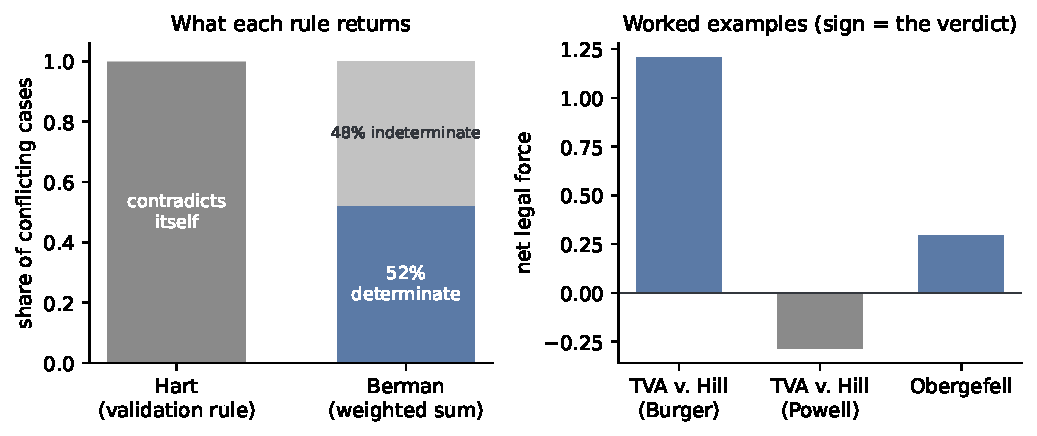
\includegraphics[width=\textwidth]{F1_static_saw}
\caption{The static weighted sum. \textit{Left}: on six thousand opposed
cases, the hardest conflict type, a Hartian validation rule contradicts
itself on $100\%$ of them, certifying both outcomes at once; the weighted
sum never contradicts itself, deciding about $52\%$ at $\tau = 0.2$ and
reporting the rest as unresolved. Thirty-seed means. The sum's coherence
holds as an entailment; the rule's $100\%$ is the rate on cases built to be
directly opposed, and on unstructured draws it is $45.4\%$; the determinacy
rate is measured throughout. See Section~IV.D. \textit{Right}: net legal force
on three worked examples, the sign giving the verdict. \textit{TVA v.\
Hill} returns $+1.205$ under Burger and $-0.285$ under Powell, opposite
determinate verdicts on one statute, and \textit{Obergefell} returns
$+0.295$.}
\label{fig:f1-static}
\end{figure}

Run through the stipulated weights of Part~II, these three disputes would seem to show the model tracking the balance rather than
manufacturing it. \textit{TVA v.\ Hill}
under Chief Justice Burger's activations produces a net force of $+1.205$, a determinate verdict. Under Justice Powell's activations the same case produces $-0.285$,
determinate the other way. That one case
lands on opposite sides of the line under two sets of activations is the opposite of
a curated demonstration: weights chosen to flatter the model would not
reproduce the split the bench actually reached. \textit{Obergefell} produces
$+0.295$, determinate.\footnote{The full \textit{TVA} activation table appears
in Part~II; Figure~\ref{fig:f1-static} reports only the resulting net
forces.}

The validation rule has been the Hartian foil of this Section, the natural one for
a test of conflict. The next Section turns to a second and more generous
Hart, for a different question: not whether a validation rule contradicts
itself, but how much law a Hartian rule leaves unsettled.

\subsection{The Model Delivers More Law Than Hart}

Berman's third claim is that a balance of principles yields more determinate
law than positivism's rule-based alternatives, answering Dworkin's worry that
positivism leaves too much of the law unsettled. I implement the Hartian
baseline in two versions and compare determinacy across thirty seeds.

The first is the more generous Hart just promised, a \textit{hierarchical Hart},
which sorts principles
into tiers by category, the two textual principles on top, the three
structural ones including precedent below, and the four moral ones below
that. It decides a case at the highest tier that contains an active principle,
and only where enough of that tier's active principles point the same way.\footnote{The
structure is more generous than a flat consensus model, in that it gives Hart
a priority system rather than a single bar across all nine principles. That
structure does not by itself buy determinacy: at a matched sixty-percent bar
the tiered rule decides $0.590$ of cases against the flat rule's $0.592$, and
less than the flat rule on nineteen of thirty seeds. What the tiering buys
Hart is faithfulness, not a higher rate. It remains a simplification of Hart's actual theory, which is
considerably more nuanced about the rule of recognition. See Hart,
\textit{supra} note 1, at 94--99. The tiers come from the exogenous category
map, never from any emergent weight, so the comparison does not lend Hart the
model's own output.} The other is a \textit{consensus Hart}, which decides
only when the share of principles pointing one way clears a bar set between
fifty and eighty percent.

Part~III's more-law-than-Hart requirement is scored against the hierarchy, which is the most
structurally faithful rendering of a rule of recognition I can construct. It
is not the most determinate of the Hartian rules, and the ranking is worth
stating plainly. It out-decides the consensus rule at bars of seventy and
eighty percent, matches it at sixty to within two thousandths, and falls well
short of it at a bare majority, where the consensus rule decides more cases
than the weighted sum itself does. Scoring the requirement against the
hierarchy is therefore a demanding choice on two of the four bars, a wash on a
third, and a
generous one on the fourth, and the bare-majority comparison is reported below
rather than folded into the requirement.

Given faithful weights, the weighted sum decides $86.2\%$ of cases ($95\%$
CI $[85.8\%, 86.6\%]$). Its margin over the hierarchical Hart is $+0.272$, positive on every seed.
That figure is a mean across thirty seeds at the moderate weight distribution,
and it would likely shift under a different case distribution. Against the
consensus Hart the margin depends on the bar, and there is a single exception.
Only when the rival is relaxed all the way to bare-majority counting do the
two draw even ($-0.021$, a dead heat, and on the conservative baseline at
that); ask for any more agreement and the weighted sum wins outright, by
margins that widen as the demand rises: $+0.270$ at sixty percent, $+0.589$
at seventy, $+0.786$ at eighty.\footnote{Each of those three margins is
positive on every one of the thirty seeds, and the bare-majority margin is
negative on twenty-eight of them. Part~III's requirement is scored against the
hierarchical Hart, where the advantage is uniformly positive.} The only competitor that out-decides the weighted sum does so by relaxing its
demand for agreement to a bare majority, declaring the law settled wherever a
simple majority of the principles in play agree. A defender of counting would
presumably not accept that as a trade. That exception seems telling rather than damaging.

That margin is the answer to Dworkin. But it comes with a condition that
belongs in the open rather than in a footnote, since it is measured on
independent activations.

Under the category-correlated activations this
Article elsewhere calls realistic, the comparison reverses: the
hierarchical Hart decides $95.6\%$ of cases against the weighted sum's
$90.1\%$, and the margin runs to $-0.054$.\footnote{Thirty seeds.
Independent activations: hierarchical Hart $0.5925$, weighted sum $0.8605$,
margin $+0.268$. Category-correlated: hierarchical Hart $0.9558$, weighted
sum $0.9015$, margin $-0.054$. Part~III scores the requirement on
independent activations, where the advantage is positive on every seed.}
About what the reversal measures it is worth being exact. It is not that a
tiered rule finds more law, but that a tiered rule decides faster by
consulting less. On the same battery the weighted sum brings about eight
of the nine principles to bear. The hierarchical Hart brings $1.83$ of the nine,
because its top tier is dispositive on $95.7\%$ of cases and it never
reaches the rest. In all, the force it never reaches is roughly three-quarters of the force
in play.\footnote{Principles carrying nonzero activation that
each rule actually consults, averaged over the battery: weighted sum $8.10$
of nine on independent activations and $7.72$ on correlated; hierarchical
Hart $1.83$ on both. Share of total weighted force never reached: weighted
sum $0$; hierarchical Hart $0.780$ independent, $0.761$ correlated. The top
tier is dispositive on $95.7\%$ of cases.}

Correlation makes that cheap. Where principles in a category fire
together, the top tier more often points one way on its own, so a rule that
stops there stops sooner and more often. Determinacy counted by itself therefore rewards foreclosure, and a
rule can win the count by declining to hear the conflict the theory is
about. On this evidence that is arguably a reason to read the raw determinacy
comparison with care, though not a reason to discard it. The balance of principles still settles more of
the law than the rule-based picture does, wherever that picture actually
engages the conflict, and it settles most where rules collide and run
out.

Dworkin's charge has a sharper form, and it is Ruth Chang's. Berman's
published defense offers a dispute in which his account is determinate and
Hart's plausibly is not. To that Chang objects that winning a particular
case establishes nothing about the net tally. An account can be determinate where
its rival is silent and silent where its rival is determinate, and only a
count across the run of cases can say which delivers more. Berman records
the objection and accepts it.\footnote{Berman, \textit{Practices},
\textit{supra} note 7, at 347 n.144 (conceding that a model yielding ``a
legally determinate rule in this dispute, while the orthodox Hartian model
does not,'' would ``still not establish that it yields more determinacy all
things considered,'' since ``some disputes that appear determinate on the
Hartian account might become underdeterminate through the principled
positivist lens,'' and that ``this is not something we can net out a
priori''). Chang holds the Chair of Jurisprudence at Oxford, which Hart
and Dworkin held before her. See also E-mail from Mitchell N.\ Berman to
author (Mar.\ 2026) (on file with author) (directing attention to the
note).}
% RESOLVED 18 Aug 2026. The pin cite was read directly from
% Docs/Writing/JESP-28-3-A1-Berman.pdf: n.144 begins on journal p.347 and runs
% onto 348. Quotation in the footnote is verbatim from that note.

This Part counts across the run of cases. Both rules see the
same battery, case by case, and the margin is the difference between them.
On that measurement, taken on the independent activations the requirement is
scored under, the weighted sum out-decides the hierarchical Hart by $+0.272$,
on every one of thirty seeds. Chang's is the question this design
answers, and it is answered in the form she put it.

Three conditions travel with the answer, and none is a formality. The count
is net across a distribution of cases, and these cases are synthetic, so
the margin shows that the weighted sum out-decides this Hart on
this battery rather than on any real docket. The count is also net against
a particular Hart: relaxed all the way to bare-majority counting, the
consensus Hart decides more. And the count is net under a particular
activation structure, which is the condition that bears hardest. Change the
structure to the correlated one and the margin reverses. Chang's worry is
therefore met on the terms she set, on the design Part III specifies, and
not in a form that would survive every way of generating the cases. That is
a narrower answer than the margin alone suggests, and it is the honest one.

On how to settle such a question Berman concedes that no armchair will do,
and proposes attending to real cases as an insider to the practice.
Modeling is a third route. Its advantage is that both rules can be put to
identical inputs, which no survey of real cases can arrange, since only one
legal system is actual and its docket is the one that system generated. Its
cost is that the inputs are stipulated. Neither route dominates the other,
and they would appear to answer different halves of what Chang asked: modeling
can hold the inputs fixed, and attending to real cases can say what the inputs
really are.

The size of the advantage is a finding in its own right; Part~III asks only
that it be positive, and it is, on every seed. And it sets a benchmark for
the rest of the Article. Any mechanism that grounds the weights in
practice, rather than stipulating them, would have to preserve this margin
to claim the same payoff. Parts~V and~VI report that the emergent mechanisms do, though by margins
that differ more than one might expect.

\subsection{The Model Weighs Magnitude}

Principled positivism is a theory of weighing rather than a dressed-up
ranking because a principle contributes force in proportion to how
strongly it applies, not to where it ranks. Berman is explicit on the point.\footnote{Berman, \textit{Practices}, \textit{supra} note 7, at
311--13, 333.} The weighted sum has this property. On the magnitude probe of Part~III, a
perturbation that changes only the magnitudes of the activations, holding
every sign and within-case rank fixed, the ungated sum, which decides on the
bare sign of net force, changes its verdict about $9.7$ times
as often as a lexical rule on the same weights ($0.0256$ against $0.0026$),
and the gated sum this Article runs elsewhere, whose net force must also clear
the determinacy threshold, about $19$ times ($0.0502$
against the same $0.0026$).\footnote{A rank-only rule is near-blind to a magnitude-only
perturbation by construction, so its near-zero score is partly definitional;
that the weighted sum responds substantially is not, and that is what the
requirement credits. Part~III's five-fold bar sits well below the observed
near-tenfold gap.} The model reads the magnitudes; it does not merely count
which side holds the top-ranked principle.

Whether that advantage rests on cardinal information an ordinal model would
discard, and whether it survives across the whole family of magnitude-weighing
rules, are the questions of Part~VII. For now the narrow claim suffices: the
static model weighs magnitude, as the theory requires.

\subsection{Which Claims Are Theorems, and How Far They Reach}

Some of the properties established above do not depend on the draws of any
particular run. They can be proved of the model as such and checked against
the implementation as closed forms. Promoting them from findings to theorems is worth doing, because a
favorable simulation can be doubted as a lucky configuration and an entailment
of the aggregation form cannot.

The promotion has to be done carefully, though, because the five results
collected in Table~\ref{tab:theorems} are not proved in the same sense as one
another, and the differences between those senses are load-bearing. The five
are numbered here in the order the table gives them, and the Parts that follow
cite them by those numbers. Some are entailments
of the form, true on any case distribution whatever. One is a conditional.
Its consequent follows whenever the antecedent holds, and the frequency of
the antecedent remains a separate question about the cases that arise. One
is a closed form derived under a stated assumption about the distribution,
which does not survive that assumption's failure. And one is proved for a
single mechanism. Reporting all five under the bare word ``theorem'' would
obscure the distinctions that make the word worth using.

\begin{table}[t]
\centering
\small
\caption{The five results, and the scope each is proved under.}
\label{tab:theorems}
\begin{tabular}{p{0.44\textwidth} p{0.48\textwidth}}
\toprule
\textbf{What is proved} & \textbf{What the simulation adds} \\
\midrule
The weighted sum returns one verdict on any case whatever. A rule certifying each direction separately returns two whenever at least two principles apply strongly each way, which is a condition on the case and not on the rule. & on the directly opposed battery, where that condition holds by construction, the rule contradicts itself on 100\% of cases and the sum on 0\%; the condition itself obtains on 45\% of independent draws, 11\% of category-correlated ones, and 0\% under full correlation \\
\addlinespace
In the reliance mechanism, conferred weight is a function of pressure and activations and not of invocation propensity. Not proved for uptake, where weight is invocation frequency by construction. & two runs differing only in invocation frequency confer identical weights, to a difference of 0.000, though their uptake shares differ \\
\addlinespace
The weighted sum responds to a change in magnitude alone; a rule reading only ranks cannot. & magnitude sensitivity 0.023 for the sum against exactly 0.000 for a rank-only rule with no activation cutoff, and 0.0024 for the implemented foil, which carries one \\
\addlinespace
For activations drawn independently and uniformly, net force has variance $\tfrac{1}{3}\sum_i w_i^2$ and the determinacy rate is $2(1-\Phi(\tau/\sigma_F))$ under a normal approximation. Not proved for correlated activations. & simulation matches the formula to within 0.006 on the grid tested here, and 0.0106 on the finer grid of Part VIII; both residuals measure the approximation rather than the implementation \\
\addlinespace
With equal weights the sum and a vote-count disagree on a set of positive measure. The proof is a counterexample and supplies no rate. & on nine principles the two disagree on 15.4\% of cases, reproduced at 15.3\% on the separate implementation of Part VII \\
\bottomrule
\end{tabular}

\end{table}

The first result is the single-valuedness behind the contrast this Part opened
with, and two claims travel together in it that are not equally strong. That
the weighted sum never certifies both outcomes is an entailment: net force is
one real number, its sign is one value, and no distribution of cases can
disturb that. That a validation rule certifies both is a conditional. Such a
rule does so whenever at least two principles apply strongly in each
direction, which is a condition on the case rather than on the rule.

So the $100\%$ in Figure~\ref{fig:f1-static} is the rate on a battery of
directly opposed cases, built so that every case satisfies the condition, which makes the
figure definitional rather than measured. Where cases are not built to satisfy
the condition, its rate can be measured. On independent
draws it obtains on $45.4\%$ of cases; under the category-correlated
activations this Article treats as realistic, on $10.5\%$; under full correlation, on none of the draws tested, since principles that
move together rarely point strongly both ways.\footnote{Thirty seeds of four
thousand cases each, against the same validation rule used throughout, which
counts a direction validated when at least two principles reach an activation
of $0.5$. The $100\%$ figure is the same rule on the opposed battery of
Section~IV.A.} Full correlation is the structure in which a single factor
moves all nine principles together rather than only those of a kind.

That spread strengthens the argument rather than weakening it. The
contradiction is not a defect that afflicts a validation rule at some fixed
rate across the run of cases. It afflicts the rule precisely where principles
genuinely collide, and it disappears where they line up, which is where nobody
needed an aggregation rule in the first place. The weighted sum's coherence is
therefore worth most exactly where the rival fails, and worth nothing where
the rival does not. That is a sharper claim than a rate, and it is the one the
theory needs.

The second result severs a principle's weight from how often it is invoked,
and it is proved for the reliance mechanism of Part~III, which confers weight
on a principle through the precedent that comes to rest on it. There the
weight conferred is a function of case-level factors and of whether the
principle prevailed on the winning side of a contested dispute, which turns on
the exogenous pressure behind it and on the activations. How often the
principle is invoked appears nowhere in the expression. Two runs differing only in
invocation frequency confer identical weights, to a difference of $0.000$,
while their uptake shares, which track invocation directly, differ.

The scope cannot be dropped. Under the uptake mechanism a principle's weight
simply is its invocation frequency, so there the two quantities are not merely
dependent but identical. The result therefore establishes not that
weight never tracks mention, but that it need not, and that a practice-based
theory has to say which of the two it means. Parts~V and~VI take up that
question, and the divergence they report is in large part this one.

The third promotes magnitude-weighing from observation to entailment. The sum
responds to a change in magnitude alone ($0.023$) where a rule reading only
ranks cannot respond at all (exactly $0.000$). That the rank-only rule scores
zero is definitional, as noted above. That the sum responds at all is not. Measured
instead against the implemented lexicographic foil, which carries a small
activation cutoff, the foil itself responds at $0.0024$ rather than at exactly
zero.\footnote{These are the analytical notebook's own battery. Section~IV.C reports the same
two quantities from the static battery, at $0.0256$ against $0.0026$. The
levels differ with the draw; the ratio does not, standing at $9.75$ here and
$9.70$ there, and Part~VII reconciles the two runs directly. See infra
Part~VII.A.}

The fourth gives the determinacy rate as a closed form in the threshold, and
it is the one result here that carries a distributional condition it cannot
shed. Where activations are drawn independently and uniformly, net force has
variance $\tfrac{1}{3}\sum_i w_i^2$, and across nine principles the central
limit theorem puts the determinacy rate at $2(1 - \Phi(\tau/\sigma_F))$, where
$\sigma_F$ is the standard deviation of net force, a different quantity from
the critical uncertainty $\sigma^{*}$ used above, and $\Phi$ is the standard
normal distribution function. The
simulation matches that formula to $0.006$ on the grid used here and to
$0.0106$ on the finer grid of Part~VIII.

Both residuals measure the quality of the normal approximation rather than the
fidelity of the implementation, which is worth stating plainly, because a
closer match would not be a better result. Neither the independence assumption
nor the approximation is idle. The weights enter only through the single scale $\sigma_F$, and that
separability lets Part~VIII treat the threshold analytically, but it is separability under independence. Where activations are
correlated the variance is not $\tfrac{1}{3}\sum_i w_i^2$, and the formula
does not apply.\footnote{Part~VIII's threshold analysis is conducted on
independent activations for this reason. The qualitative finding it reports,
that the determinacy curve is smooth and monotone with no privileged value,
does not depend on the closed form, and Section~VIII.A confirms the
monotonicity directly.}

The fifth is that equal weights are not vote-counting, and here the proof is a
counterexample. Three principles activated at $(0.9, -0.4, -0.4)$ give the sum
a positive verdict and the count a negative one, which establishes that the
two rules disagree on a set of positive measure. It establishes no rate. The $15.4\%$ in Table~\ref{tab:theorems} is a simulation over nine principles,
and Part~VII reproduces it at $15.3\%$ on a separate implementation. Those two figures
check each other, which is worth having, but neither is entailed by the
counterexample and the proof would stand if both were much smaller.

The counterexample does settle the qualitative point the theory needs,
since Berman is explicit that his account permits equal
weights.\footnote{Berman, \textit{Practices}, \textit{supra} note 7, at
323--24.} Even at that limit the sum is still reading magnitudes the count
discards, so equal weights do not collapse the model into majority rule, and
that is why the theory can tolerate them at all.

Stating these results in their proper scope earns the word ``sound,''
and the scope is narrower than the word on its own suggests.
Magnitude-weighing and the equal-weights counterexample hold on any activation
distribution whatever, so the objection that synthetic cases prove nothing
cannot reach them, though the counterexample establishes only that a
disagreement has positive measure and not how large it is. The
single-valuedness result divides, its universal half belonging to the weighted
sum and its conditional half to the rival. The independence of conferred
weight from invocation is bounded by mechanism rather than by distribution,
holding for reliance and failing for uptake. Only the closed form for the
determinacy rate is conditioned on the distribution itself, and there the
condition fails on exactly the correlated activations the later Parts treat as
realistic.

That is a substantial result and not a universal one, and the difference is
worth keeping in view, because the Parts that follow turn on distributional
structure the static analysis assumes away. None of the five settles
where the weights come from. Each takes them as given. That is the question
the next Parts inherit, and it is likely the harder one.

\subsection{What the Static Case Establishes}

Given faithful weights, then, the static model meets every requirement. Rough weights suffice: it absorbs about $\pm 0.09$ of weight error, and
better than twice that on the correlated activations of real cases, where a
paired run rises from $0.069$ to $0.156$. Conflicting principles coexist. At a demanding threshold the model decides
a majority of opposed and balanced cases, and on the bare sign of net force
nearly all but true equipoise. Through aggregation it resolves the
conflicts on which a validation rule contradicts itself. On Hart, the determinacy margin over the charitable hierarchical baseline is
$+0.272$ on independent activations, positive on every seed and wider against
stricter consensus competitors, and it reverses under the correlated
activations of realistic cases. And the model weighs magnitude, responding to
how strongly principles apply about ten times as much as a rule that merely
ranks. Several of these properties hold as theorems, though not all in the
same sense, and not all of them universally.

The stipulated engine is therefore sound. The prior question, the practice
conferring the weights it runs on and the forces driving them to change, is
where the rest of the Article turns, beginning with Part~V. Two threads run
forward as well, both taking the weights as given. Part~VIII asks what governs
how much law the model declares determinate, and how sensitive that is to the
one parameter the theory does not fix. Part~VII asks how far its
magnitude-weighing separates it from ordinal alternatives, and whether the
result survives across the family of aggregation functions.


% Authorship: Claude-drafted, author-revised
\section{Weights Can Emerge from Practice}

Part IV took the weights as given and asked the aggregation Berman
describes to do the work the theory needs. It does. But that leaves the
theory's central commitment untested. On his own account Berman does not say that a philosopher supplies the
weights. He says practice confers them.\footnote{Berman, \textit{Practices}, \textit{supra} note 7, at
329.} On stipulated weights alone, a model shows only how the law would come out if
a theorist set its parameters, and principled positivism makes no such claim. So the prior question is whether a weight
structure of the sort Part IV ran on can arise from practice rather than
being written down in advance.

Through the simplest of the four practice mechanisms, this Part shows that it can,
and that the weights it yields clear the same bar the stipulated ones did. That is a proof of concept, not the whole story. As implemented here the mechanism is a spare one, and Part VI shows that
richer mechanisms confer weight differently. But the possibility must be
established first, and it is established here.

The mechanism is the \textit{uptake} model of Part III. In nine-judge panels, a bench of roughly one hundred simulated judges
decides a stream of cases. Each judge on the bench carries one of four interpretive
methodologies, and the methodology sets the larger part of how readily that
judge reaches for each principle. Nothing about
the weights is stipulated. The emergent quantity is each principle's \textit{uptake share}: how often the bench
as a whole invokes it, scaled so that the most-invoked principle sits at
$1.0$. At issue is the structure that quantity takes on once the simulation has
run its two thousand cases.

Three results follow. A stable weight structure emerges, and it splits the principles into two
groups. That split does not come from any survival contest among judges,
and so answers a caution Berman has pressed. And the emergent weights meet
all four requirements, on every way of turning the bench over that I tried,
just as the stipulated weights did. A closing section marks the limits of the
mechanism, and those limits open onto Part VI.

\subsection{A Stable Two-Group Structure Emerges}

Run the bench and let it decide cases, and the uptake shares settle into
a stable arrangement. By the end, five principles stay \textit{live}, accumulating high uptake:
text, original meaning, precedent, structure, and
federalism. Those are the textual and structural principles, keyed to the
constitutional text and its architecture. Four go \textit{dead}: dignity,
equality, liberty, and welfare, the moral principles. They are not
unmentioned. Their raw uptake shares run from
about $0.35$ to about $0.50$ against $0.79$ to $1.00$ for the other five. Beyond
that difference, the live/dead cut zeroes any principle whose share falls below the
median of the nine, and the moral four fall on the wrong side of it, a point
Part VI returns to.

This membership is not a close call that tips one way
on some runs and the other way on others. Each seed is one independent run of
the simulation, and on every seed the same five are live and the same four are
dead; as the next Section develops, the same holds under every rule for
retiring and replacing judges. The structure is an output of the model, not an input to
it, and it is the same output every time. Whether a real bench would sort
the same way is not something this design can show.

Why these five? The answer is the practice-grounding idea doing its
work. The simulated bench is composed in equal quarters of four methodologies:
textualist, originalist, purposivist, and pragmatist. Each sorts the nine
principles into a band it reaches for readily, a band it reaches for
reluctantly, and a middle band. Two of them, the
textualist and the originalist, reach for the textual and structural
principles far more often than for the moral ones. Together those two methodologies make up half the bench, and both reach for
all four moral principles less readily than for anything else on the list,
while no moral principle is a favorite of more than one of the four. So the
moral principles accumulate the fewest invocations.

The principles that accumulate the most, though, are not the ones any
methodology favors most intensely but the ones the bench as a whole is willing
to take up. Although only one methodology favors precedent, it takes the
highest share of the nine, because none disfavors it; and structure survives
comfortably although none favors it at all, for the same reason. Favored
intensely by two methodologies and disfavored by the other two, original
meaning sits at the bottom of the live group. Breadth of tolerance governs,
not depth of preference.\footnote{On the static bench, averaged across the thirty seeds,
the shares are precedent $1.00$, text $0.96$, structure $0.85$, federalism
$0.82$, original meaning $0.79$, then welfare and liberty at $0.50$ and
dignity and equality at $0.35$. Because shares are scaled to the most-invoked
principle, precedent's $1.00$ records which principle leads rather than by how
much; it leads on every one of the thirty seeds, and original meaning is the
lowest live principle on twenty-eight of them. The ordering is the one the
bench-wide average of the four methodologies' invocation propensities
predicts, and that average is fixed before any case is decided: no methodology
places precedent or structure in the band it reaches for least, while each
moral principle falls into that band for at least two.}

The live/dead line falls exactly where the
composition of the bench places it. Practice confers the weight here, and argument does
not: the moral principles
are not ranked lower because they matter less, but because this bench
takes them up less. Change the composition enough and the line moves with it.
Hold everything else fixed and reseat the bench so that the purposivist
methodology, the one most disposed toward the moral principles, holds a majority
of the seats rather than a quarter, and dignity, equality, and liberty come up
live while text, original meaning, and federalism go dead.\footnote{Thirty
seeds per composition on the static bench, with the live/dead cut in place and
everything else as in the headline run. Equal quarters reproduce the headline
result on all thirty seeds. Raising the textualist share to $55\%$ leaves the
live set unchanged on all thirty and widens the cluster gap defined just below
to $0.585$, the principles a textualist bench favors having been live already.
Raising the purposivist share to $55\%$ instead trades three principles for
three on all thirty, at a cluster gap of $0.444$. Precedent and structure stay live throughout and welfare stays
dead, which is what the breadth-of-tolerance reading predicts. What
composition moves is the membership of the two groups, not the two-group
shape.} That result is worth holding onto, because it ties the emergent
structure to how a bench is staffed: who sits on the bench decides which
principles carry weight, a thread the Conclusion picks back up.

The two groups are far apart. The \textit{cluster gap} is the distance between
the average live share and the average dead share, and it runs to $0.461$ on
the bench
where no judge is ever replaced, which is the bench carrying the headline
result, and to $0.512$ averaged across all four rules for turning the bench
over.\footnote{The gap is the difference between the mean uptake share of the
live principles and the mean uptake share of the dead principles, averaged
across the thirty seeds in each of the four turnover regimes, so across one
hundred twenty runs in all; uptake shares run from $0$ to $1$, so a gap of
$0.512$ separates the two groups by more than half the available range. The
figure is pulled up by the fitness regime, which replaces the least decisive
judges with copies of the most decisive and which the design is built to do
without: on the static bench, which carries the headline result, the gap is
$0.461$ (Section V.B). The membership
of the two groups, which five principles are live, is identical on every
seed.}

A word on how firm that two-group reading is, because the honest answer has
two sides. Run by run the evidence is thinner, and two tests of it disagree
about how much thinner. Within a single run the distribution under test holds
nine numbers, one uptake share per principle, which is a thin basis for
telling one hump from two. Hartigan's dip test, which measures the largest
distance between the observed distribution and the closest single-humped one and
assumes nothing about the shape of the humps, rejects the one-hump null on
sixty-six of one hundred twenty seed-runs. A Gaussian-mixture criterion instead compares the
fit of two bell curves against one, and rejects on three.\footnote{J.A.\ Hartigan \& P.M.\ Hartigan, \textit{The Dip Test of
Unimodality}, 13 \textsc{Annals Stat.}\ 70 (1985). The mixture criterion
counts a run as two-humped when the two-component fit beats the one-component
fit by a Bayesian-information-criterion margin above ten and the component
means sit at least one standard deviation apart. The dip figure is pulled up
by the fitness regime, where it rejects on all thirty runs at a median $p$ of
$0.007$. Across the other ninety it rejects on thirty-six, and on the static
bench that carries the headline result it rejects on eleven of thirty, at a
median $p$ of $0.058$, which falls on the other side of the conventional
line.} The distance between sixty-six and three is a small sample acting
on two tests of different sensitivity, not a fact about the weights. Neither per-run
figure should carry the claim.

Pool the shares across seeds, though, and both tests agree, decisively. On
the pooled distribution the dip statistic is $0.074$ and the one-hump null
is rejected beyond any conventional level, the two-component fit beats the
one-component fit by a Bayesian-information-criterion difference of $664$
where a difference above ten is already strong, and the bimodality
coefficient, a standard index of two-groupedness, sits well into the range
that marks a genuinely split distribution. On the static bench alone, which
carries the headline result, the dip statistic rises to $0.128$. Both tests
establish that the pooled distribution is not a single hump. That is weaker
than establishing that it has exactly two.\footnote{Neither test counts
modes. The dip test rejects unimodality without saying how many humps replace
it, and the mixture criterion here compares only a two-component fit against a
one-component one. Allowed more components on the same pooled shares, the
Bayesian information criterion keeps improving past two. The two-group reading
is carried by the live/dead structure the next Sections trace, not by the
mixture comparison. The bimodality coefficient runs from $0$ to $1$, with
values above about $0.55$ taken to indicate two groups; on the pooled shares
it is $0.657$.} The claim, then, is modest: a stable two-group separation in the emergent
weights, visible in the pooled behavior of the bench and not established by
any single run. That is the claim the rest of the Part uses, and no more.

\subsection{The Separation Is Composition, Not Selection}

Berman has cautioned against reading his account through a Darwinian
lens, in which weights are fixed by some survival-of-the-fittest contest
among principles or among the judges who carry them. The caution is well
taken, and this mechanism is built to respect it, as a single comparison
shows.

The design lets the bench turn over in four ways. In
the first, the \textit{static} bench, no judge is ever replaced and none
is selected for anything: the same hundred judges decide every case from
first to last. The other three retire and replace judges over time: by appointment, reseating
a random fifth of the bench with judges drawn afresh from all four
methodologies in equal proportion; by drift, reseating a random fifth with
near-copies of other sitting judges; and by a fitness rule that retires the
least decisive judges, measuring decisiveness by the absolute size of a judge's
own force in a case, and refills their seats with copies of the most decisive.
Appointment here names one of these rules for turning this bench over, not the
appointment mechanism of Part III, which grounds weight in a different
quantity altogether. Of the four, only the fitness rule rewards success, and
it is the one whose framing Berman questions.

On the evidence here, the separation does not need selection among judges at
all. On the static bench, where no judge is ever replaced and none is selected
for anything, the two groups pull apart by a cluster gap of $0.461$. Turning the bench over by drift, or by appointment, barely moves that figure
($0.452$ and $0.472$). The fitness rule does move it, widening the gap to
$0.663$, and the reason is instructive. It does not sharpen a fixed bench. It
destroys the bench's composition: replacing the least decisive fifth with
copies of the most decisive drives the purposivist methodology extinct on
every one of the thirty seeds and the pragmatist on twenty-nine, leaving a
bench roughly four-fifths originalist and one-fifth textualist.\footnote{Final
composition after two thousand cases, thirty seeds. The static, appointment,
and drift regimes all finish within a seat or so of the twenty-five each they
began with; the fitness regime finishes at $79.7$ originalist, $20.2$
textualist, and none of the other two.} So the widest gap of the four belongs
to the bench with the least methodological diversity, exactly as the
composition comparison above would predict. The fitness regime is not evidence that
selection produces the separation. It is evidence that selection produces a
narrower bench, and a narrower bench sorts more sharply.\footnote{Cluster gaps by turnover regime, averaged across seeds: static $0.461$, drift
$0.452$, appointment $0.472$, fitness $0.663$. Tested against the static
bench, only the fitness regime differs to a degree unlikely to be chance ($p =
2\times10^{-9}$); appointment is marginal ($p = 0.043$) and drift is
indistinguishable ($p = 0.18$). The membership of the two groups is the same
under all four regimes.}

Where the split appears settles the question. If it were an artifact of a
survival contest among judges, it would show up only under the fitness rule
and be absent from the static bench, where no such contest is ever run. On the
static bench it is present at a gap of $0.461$, and the one regime
that runs a contest produces its larger gap by narrowing the bench rather than
by ranking principles. The separation traces to the composition of the bench, to the mix of
methodologies and how readily each reaches for each principle, rather than to
any winnowing of judges as such. Winnowing matters only where it changes that
mix. The fitness regime changes it; appointment and drift do not. So
the live/dead line is drawn by which principles a given bench is disposed to
take up, a standing fact about the practice rather than the outcome of a
contest. This is arguably the reading Berman's caution asks for. Nothing in the result depends on selecting among
judges, and the headline separation is the one that holds on the bench where
no judge is ever retired.

One reinforcement does remain, and it should be named rather than left in the
code. A judge's readiness to invoke a principle is not fixed by methodology
alone: a small part of it tracks the weights the bench currently carries, so a
principle the live/dead cut has zeroed is thereafter reached for less often.
That is a rich-get-richer dynamic among principles, and it runs on the static
bench along with the others. Its effect is measurable and modest. The five
live principles settle exactly where the methodology mix alone would put them,
while the four dead ones settle about a fifth lower than it
would.\footnote{Comparing the emergent shares against the bench-wide average
invocation propensity, which is fixed before any case is decided, the five
live principles come in at $1.00$ of the predicted value on average and the
four dead ones between $0.795$ and $0.798$.} So
the contest among judges that Berman's caution rules out is absent. In its
place is a feedback among principles that widens a gap the composition of the
bench had already created.

\subsection{The Emergent Weights Meet the Four Requirements}

Practice-grounded weights must clear the same bar as stipulated ones, and,
held to the four requirements of Part III, they seem to.
On the runs reported here they meet all four, and under every one of the four
turnover regimes.

First, they are \textit{well-defined}: the surviving set is nondegenerate and
identical on every seed and under every turnover regime. How many survive,
five here, is not itself informative, since the live/dead cut sits at the
median of nine and so leaves five standing as a matter of arithmetic. The
requirement asks only that at least two principles carry weight above a small
cutoff, and what these runs add beyond that is the stability of the surviving
set rather than its size.

Second, they are \textit{noise-tolerant}. The emergent weights absorb Gaussian
weight error up to a critical uncertainty, the level at which more than one
case in five changes its verdict, and that level averages between $0.091$ and
$0.097$ depending on the turnover regime, which sits above the $0.07$ floor of
Part III.\footnote{Those two figures are the spread of the four regime means. The
requirement is scored run by run, and run by run the emergent critical
uncertainty ranges from $0.075$ to $0.113$ across the hundred and twenty runs,
so the worst single run clears the floor by $0.005$ rather than by the margin
the regime means suggest. Recall too that the floor is the lowest cell mean of
Part III's forty-five-configuration grid, not the stipulated engine's worst
run, so clearing it does not establish that an emergent mechanism is more
noise-tolerant than the stipulated engine at its worst.} Third, they
\textit{weigh magnitude} rather than merely rank, passing the magnitude probe,
which perturbs only the magnitudes of the activations and asks whether the
verdict changes; the stipulated engine passed the same probe. Fourth, they deliver
\textit{more law than the hierarchical Hart}: the determinacy margin over
that charitable baseline runs to about $0.267$ to $0.271$, positive on
every seed, the same $+0.27$ the stipulated engine posted in
Part IV.\footnote{The requirements pass on every seed under all four
turnover regimes: well-defined, noise-tolerant, magnitude-weighing, and
more-law-than-Hart each hold for the static, drift, appointment, and fitness
benches alike. The margin over the hierarchical Hart is
$0.267$ to $0.271$ across regimes, matching the stipulated engine's
$+0.272$ from Section IV.B.}

The practice-grounded margin lands on the stipulated engine's own figure, but
that coincidence carries less information than it appears to. The hierarchical
Hart consults only the activations and the category tiers, never the weights,
so its determinacy rate is the same whichever weight vector it is compared
against. The margin is therefore the weighted sum's own determinacy rate less
a constant, and that rate is nearly flat across any weight vector that is not
degenerate. The two margins could hardly have failed to agree here. The
requirement establishes that the emergent weights are nondegenerate. That is
worth knowing, though the first requirement had already asked nearly the same
thing. The
margin is also measured on independent activations alone, and Part IV reports
that it reverses under the correlated ones.

Across the full weight vector the spread is wide. The vector's coefficient of
variation, a scale-free measure of how spread out the weights are, sits near $0.90$. But that spread is the live/dead split showing up as a
statistic, not graded variation among the live principles.\footnote{Among the
five that survive, the weights run from $0.79$ to $1.00$ and their coefficient
of variation is $0.09$, which is tighter than any of the other three
mechanisms manages across its own nine. \textit{See infra} Part~VI.B.}

This matters for the scope of the claim. Part III
was explicit that gradation, weights finely spread rather than
clustered, is measured but not required, because Berman permits
principles to carry equal weight.\footnote{Berman, \textit{Practices},
\textit{supra} note 7, at 323--24.} So a structure that sorts principles
into two groups without grading finely within them is not a defect to be
explained away. It meets every requirement the theory imposes, and those requirements are
arguably the standard. Whether the two-group shape is the only
shape practice can produce is a separate question, and its answer is no:
Part VI's other mechanisms grade their weights, and confer them
differently, which is the point of running more than one.

Two further features of the emergent weights, neither a requirement, are
worth recording. The first locates what drives the separation: how far the two
groups pull apart tracks how differently the four
methodologies reach for principles. Compress those differences, make the
methodologies reach for principles at more nearly equal rates, and the cluster gap narrows. Read off the raw uptake shares with the live/dead cut
switched off, the gap runs $0.135$ when the methodologies are close, $0.257$
when moderately spread, and $0.361$ at the wide spread the headline bench
uses. The size of the separation, then, is driven by how far apart the
methodologies' invocation tendencies lie, a different lever from the mix of
seats the composition sweep varied.\footnote{Cluster gap by the spread of
invocation tendencies across methodologies, measured with the live/dead cut
switched off: narrow $0.135$, medium $0.257$, wide $0.361$. These sit below the $0.461$ static-bench figure reported above, and the reason
is not that the cut zeroes anything: both figures are read off the uptake
shares before any principle is set to zero. What separates them is that the
cut, where it is switched on, operates while the simulation runs, so a
principle it zeroes is invoked less often in the cases that follow and the two
groups draw further apart than they otherwise would. Where the cut is placed
then governs how many principles count as live, seven surviving a lenient
placement, five the default, three a stringent one, but the underlying gap
stays near $0.44$ to $0.46$ throughout, so the clean live/dead binary is in
part an effect of where the cut falls, not a fact about the weights alone. How often the
bench turns over barely matters (a gap near $0.37$ whether it turns over
every $250$, $500$, or $1{,}000$ cases).}

Second, the bench co-invokes within categories. The distinction from Part IV
matters and is easy to lose. Part IV's correlated cases are cases in which the
activations move together, and the uptake bench does not generate those: its
case stream is drawn independently, exactly as Part IV's conservative baseline
was. The bench generates instead a pattern in which judges reach for
principles together, a fact about invocation rather than about the cases.

Nor does that pattern track the three categories evenly. Within a category,
principles are co-invoked at $0.80$ for the textual pair, $0.64$ for the
structural, and $0.55$ for the moral, on a scale where $1.0$ would mean that a
judge reaching for either always reaches for the other. Across categories the figure depends
entirely on which pairing is taken: textual with moral is $0.21$, the most
separated pairing the methodology table can produce, but textual with
structural is $0.66$, which is higher than the moral principles manage among
themselves, and structural with moral is $0.38$. Averaged over all three
cross-category pairings the ratio of within to across is about $1.6$, not the
three to one the most separated pairing suggests.\footnote{Ten seeds on the
static bench. The structure is two blocs rather than three categories: the
textual and structural principles are co-invoked at nearly the within-category
rate, and both are separated from the moral principles. That is the same
division as the live/dead line, which is what one would expect if both are
consequences of the same methodology mix.} Since the tendency to co-invoke within a category is
partly built into the methodology table the bench starts from, this is a
consistency check rather than an independent result.

Beyond those two, one measurement remains. It records how far
the panel's aggregate behavior sits from the weighted sum it is built from. It is not a test of whether the bench runs
a weighted sum, and should not be read as one: each judge's force is
constructed as a weighted sum of the principles it invokes, using the emergent
weights, so there is no rival rule it could have been running and a high
correlation was guaranteed by construction.

The comparison measures instead how far the panel's force falls short of the
full weighted sum. Because each judge sums only the principles it happens to invoke, the
panel's mean force is a thinned version of the full weighted sum over all
nine, and it runs about two-thirds the size. Correlation between the two is
$0.970$ and the root-mean-square difference is $0.42$.\footnote{The shrinkage
comes from the invocation rate and not from the determinacy threshold, which enters nowhere in
either quantity compared and which in any event could not alter a force, only
whether a case is called. Over the live principles the mean invocation rate is
about $0.63$, and the panel force runs at about that fraction of the full
weighted sum.} The one figure here that could have come out otherwise is
verdict agreement: the panel and the full weighted sum return the same verdict
on $85.9\%$ of cases, so invoking a subset rather than the whole list changes
the outcome about one case in seven. That is the quantity worth carrying
forward.

\subsection{What the Mechanism Does Not Yet Reach}

Emergence is therefore possible: a weight structure of the kind Part IV
ran on can arise from a simulated practice, meet every requirement, and match
the stipulated engine's Hart margin, without a theorist setting a
single weight, a match this Part has already said carries less information
than it appears to. That is the proof of concept this Part was asked to supply, though a proof
of concept is all it should be taken for.

Its limits mark the way to Part VI. The quantity that emerged here is
uptake share, how often the bench reaches for a principle, which is the
sparest reading of Berman's ``taking-up.''\footnote{Berman,
\textit{Practices}, \textit{supra} note 7, at 329.} In his fuller sense it is not yet weight, which a principle earns by
prevailing in contested disputes and by embedding itself in the holdings
that go on relying on it. Bare frequency of invocation is presumably a thinner thing than conferred
authority, and one would not expect the two to coincide. The reliance mechanism of Part VI models that fuller notion, and the remaining two,
the strategic and appointment mechanisms, model still others, none of which would likely
reduce to invocation counts. So this Part settles the question of possibility with the simplest
mechanism available. It leaves open the question that Part VI makes
central, whether the several mechanisms of
practice, asked to confer weight on the same principles, confer the same
weight. They do not.


% Authorship: Claude-drafted, author-revised
\section{Practice Is Not Unitary}

Part V settled a question of possibility with the simplest mechanism
available and left open the question this Part makes central. Asked to
confer weight on the same principles, do the several mechanisms of
practice confer the same weight? They do not. That is the second of
this Article's two findings. The first, from Part IV, was that the stipulated engine is sound: given
faithful weights, the weighted sum weighs magnitude, tolerates rough
specification, and leaves more law standing than the hierarchical Hart. On the
evidence below, that engine is sound in a way
that does not settle legal content, because it does not settle which
practice supplies the weights, and different practices supply different
ones.

In four steps, each turning on the one before it, the argument runs as
follows. All four mechanisms of practice clear the same bar, three of them on
every seed and appointment on twenty-six of thirty for noise tolerance. That no
mechanism fails is worth establishing, though the four requirements differ
sharply in how much they discriminate, and only noise tolerance separates the
mechanisms. Yet the four mechanisms ground the principles
differently, into weight structures that collapse to three rather than four
because two of them converge. Run over the same disputes, those structures then decide real cases
differently, reaching different verdicts about a third of the time and
opposite determinate verdicts about a quarter of the time. From
this it follows that principled positivism does not resolve the
indeterminacy it inherited from Hart and Dworkin. It relocates the question from how principles combine, settled in
Part IV, to the practice that grounds the weights, left open by the
theory.

\subsection{Four Mechanisms, One Bar}

Between them, the four mechanisms model four readings of what it is for a
principle to be taken up in practice. \textit{Uptake}, the mechanism of Part V, reads
taking-up as invocation frequency: a principle earns weight in proportion
to how often the bench reaches for it. \textit{Reliance} reads it as earned authority: a principle
gains weight by prevailing in contested disputes and by embedding itself in the holdings that go on relying on
it. \textit{Strategic} reads it as convergence under interaction:
reinforcement-learning judges, adjusting to one another, settle toward a
shared weight. \textit{Appointment} reads it as institutional inheritance:
with a near-random turnover of the bench, a principle's weight is the
decayed breadth of the still-live holdings that support it.\footnote{The appointment dynamic is not drawn from Berman's published text. It responds to his suggestion, in correspondence, that the turnover of the bench is a further channel through which practice fixes weight. E-mail from Mitchell N.\ Berman to author (Mar.\ 2026) (on file with author); see \textit{supra} Part~III.A.} Part III describes the four in full. For present purposes the point is that
each is a \textit{construal} of one phrase in Berman's account, ``taking-up,''
meaning a way of settling what that phrase picks out in a practice, and that
the four are genuinely different construals rather than variations on one.\footnote{Berman, \textit{Practices}, \textit{supra} note 7, at 329
(principles are ``constituted by the taking-up behaviors of the system's
subscribers''); see also \textit{id.}\ at 320 (fundamental legal principles
are ``grounded in practices ... by dint of legal actors taking them up in
legal decision-making'').}

That last claim carries the whole of this Part, and it needs more than one
sentence to bear it. Set each mechanism beside the text it construes.

\textit{Uptake} takes Berman at the point where he locates the constituting
relation. As he writes, principles are ``constituted by the taking-up
behaviors of the system's subscribers.''\footnote{\textit{Id.}\
at 329.} There, taking-up is described as something officials do, repeatedly, in the
course of deciding cases. Of the readings available, counting how often they do it is arguably the
most direct thing a model can make of that sentence, and it is the reading
Part V implements.

\textit{Reliance} takes up a second commitment, one Berman has pressed
harder in the later work: a principle is embedded by the holdings that go
on relying on it, so that it does not forfeit its standing the moment it
stops being mentioned.\footnote{Berman, \textit{Practices},
\textit{supra} note 7, at 310--14 (a principle embedded by the holdings
that rely on it retains vitality without current invocation); Berman,
\textsc{To Say What the Law Is}, \textit{supra} note 7 (manuscript ch.\
6).} Written out as a rule of accrual, that commitment becomes a dynamic that
confers weight for prevailing in contested dispositive disputes, amplifies
the gain by how much the resulting holding is later relied upon, decays it
over time, and strips it on overruling. Part
III calls reliance the closest of the four to Berman's own account, and
nothing in this Part revises that.

\textit{Appointment} is his in the plainest sense: he proposed it. Told
that the project modeled uptake and strategic adaptation, he replied that
the turnover of the bench is a further channel through which practice
fixes weight.\footnote{E-mail from Mitchell N.\ Berman to author (Mar.\
2026) (on file with author); see \textit{supra} Part~III.A.} To the embedding point the mechanism joins that suggestion, reading a
principle's vitality off the still-live holdings that support it rather
than off its current invocation.

\textit{Strategic} is the weak member of the set, and Part III already
says so, calling it the least Bermanian of the four, since Berman nowhere
describes judges optimizing toward a goal, and reinforcement learning brings with it a picture of adjudication he
seems not to hold.\footnote{\textit{Supra} Part~III.A (of the four mechanisms strategic is the
least Bermanian, and should be read as a robustness lens rather than as an
interpretation of the theory).} As a robustness lens, though, it arguably earns its place. Weights produced by a process Berman would not endorse, clearing every
requirement he does endorse, suggest that the requirements are not an
artifact of any one picture of practice. That is the whole of what
strategic is asked to do.

Three of the four have a warrant in Berman, then, and one is a lens. A reader
declining the lens can read the Part with uptake, reliance, and appointment
alone. With strategic dropped, a later Section reports the finding, and it looks much
the same.

Held to the four requirements of Part III across thirty seeds, every
mechanism passes, three on every seed and appointment on twenty-six of thirty for
noise tolerance.\footnote{Appointment counts as passing that requirement under
the seed share Part III states, which asks $0.80$ of seeds on noise tolerance
against $0.90$ on the other three. At the stricter share it would not clear
it. The asymmetry is in the implementation rather than in anything Berman
claims, and it is disclosed here because appointment is the only mechanism it
touches.} Each produces weights that are well-defined, that survive weight error up to
Part III's floor, that weigh magnitude rather than counting principles
lexically, and that leave a positive determinacy margin over the hierarchical
Hart. The margins sit near the stipulated engine's own advantage of about
$+0.27$: uptake near $0.27$, reliance $0.291$, strategic $0.283$, appointment
$0.284$.\footnote{Those four figures are closer together than they look. The
hierarchical Hart consults the activations and the category tiers and never
the weights, so on a given case draw it returns the same determinacy rate
whichever mechanism it is set against. Each margin is that mechanism's own
determinacy rate less one shared constant, and the weighted sum's determinacy
rate varies little across weight vectors. The clustering is therefore close to
arithmetic rather than a convergence of four independent measurements.} In the
mean, noise tolerances run from about $0.084$ to $0.097$, though the means
understate how tight the requirement is. Since it is scored seed by seed,
the binding figure is each mechanism's worst run: $0.085$ for uptake,
$0.078$ for reliance, $0.073$ for strategic, and $0.067$ for appointment,
against a floor of $0.07$.

One mechanism clears noise tolerance only barely, though, and the honest course is
to say so rather than smooth it over. Appointment meets three requirements on
every seed but meets noise tolerance on only twenty-six of thirty, its
critical uncertainty $\sigma^{*}$, the level of Gaussian weight perturbation at
which one case in five flips its signed verdict, straddling the $0.07$ floor
(minimum $0.067$, median $0.085$). That a near-random mechanism, one with no selection of any kind, only just
clears that floor is some evidence that noise tolerance is doing work. It
would be a mistake, though, to read appointment's near-miss as evidence that
the other three passes were hard-won, and the point is worth making against
this Article's own interest.

Of the four requirements, only noise tolerance discriminates among weight
vectors at all. Well-definedness asks that at least two principles carry
weight above a small cutoff, a condition almost any vector satisfies. The
magnitude probe compares the weighted sum against a lexical rule, so it tests
the aggregation form rather than the weights the form is given.
And the hierarchical Hart never reads the weights, so a positive margin over
it follows from the weighted sum deciding more cases than a tiered rule does,
as it will for almost any weights. Drawing weight vectors uniformly at
random and scoring them confirms this: on five hundred random vectors the
well-definedness test passes five hundred times and the Hart comparison five
hundred times, at margins from $+0.07$ to $+0.29$, and on a sixty-vector
subset the magnitude probe passes sixty times, never at less than nine times
the
lexical rule's rate against the five-fold bar.\footnote{Scored on the same
eight-hundred-case held-out battery the mechanisms are scored on. Even a
degenerate vector placing all weight on one principle returns a Hart margin of
$+0.19$. The hierarchical Hart's determinacy rate is bit-identical under a
zero vector and a random one, which is what one would expect of a rule that
never consults the weights.}

So three of the four requirements are properties of the aggregation form
rather than tests of a mechanism's output, and every mechanism inherits that
form by construction. Only noise tolerance asks something of the weights
themselves, and it is the one requirement that separates the four mechanisms.
The robustness result of this first step is therefore narrower than it first
appears. The formal machinery survives every picture of practice, and that is
Part IV's finding rather than a new one. The four mechanisms
are shown to share a minimum rather than a standard. This does not weaken the
Part's argument. A test that four incompatible construals all clear is a test
that cannot choose between them.

For its soundness, the weighted sum does not depend on any one picture of how
weight is conferred. That is the setup for the difficulty that follows: soundness under
every mechanism is not agreement across mechanisms.

\subsection{Three Structures, Not Four}

On the requirements the four mechanisms agree, and about everything else
they disagree. Each confers not a scalar quality of legality but a
\textit{structure}: a full vector of weights across the nine principles,
saying which count for much and which for little. Those structures diverge
sharply, and in a way that Figure \ref{fig:f2-practice} makes visible at a
glance.

\begin{figure}[t]
\centering
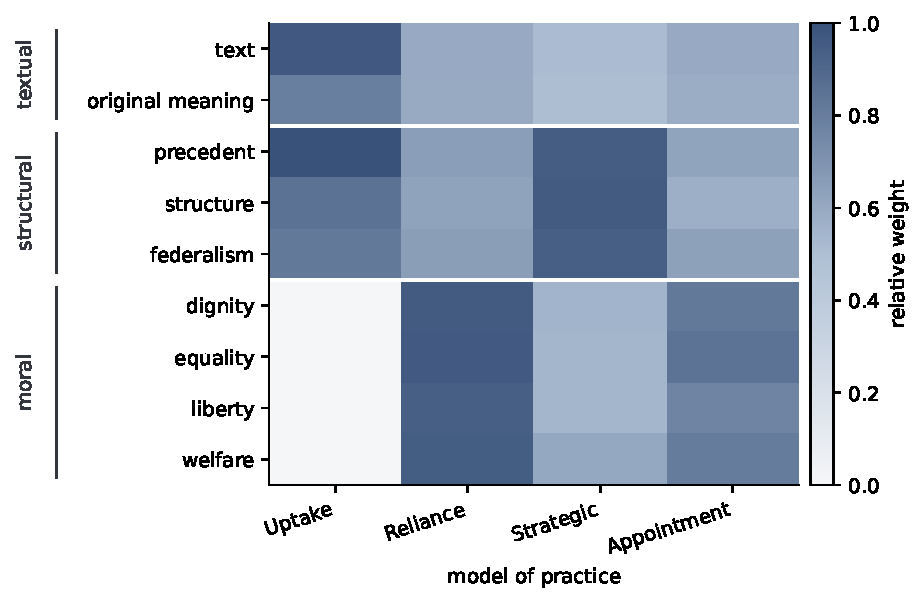
\includegraphics[width=\textwidth]{F2_practice_not_unitary}
\caption{Practice is not unitary. Across the nine principles, each column is one mechanism's emergent weight
structure; darker cells carry more weight. All four mechanisms clear the four requirements of Part III.
Uptake concentrates on the textual and structural principles and drives
the four moral principles to zero; reliance and appointment lift the
moral principles highest; strategic lifts the structural principles
highest. Reliance and appointment converge (rank correlation $+0.93$),
so the four dynamics realize three distinct structures, not four.
Appointment is the marginal mechanism on noise tolerance, clearing it on
twenty-six of thirty seeds. The heavier moral tier under reliance and
appointment is partly a category-size effect: the moral tier holds four
principles to the structural tier's three and the textual tier's two, so
under correlated activations it accrues broader aggregate force.}
\label{fig:f2-practice}
\end{figure}

Read down the columns and the structures are plainly different. Under \textit{uptake}, weight collects on
the textual and structural principles, text at $0.96$, precedent at
$1.00$, original meaning at $0.79$, structure at $0.85$, federalism at
$0.82$, while all four moral principles, dignity, equality, liberty, and
welfare, fall to zero. Of the four, uptake produces much the most concentrated
structure, its coefficient of variation, meaning spread relative to the mean,
near $0.90$. That figure is read off the vector after the live/dead cut, applied by
no other mechanism, so it chiefly registers the distance
between five live principles and four zeros rather than gradation among the
live five. Among those five the weights run from $0.79$ to $1.00$ and their coefficient
of variation is $0.09$, tighter than any other mechanism manages.

Under \textit{reliance}, the ordering nearly inverts: the moral principles sit
highest, dignity at $0.95$, equality at $0.96$, liberty at $0.94$, welfare
at $0.95$, while the textual and structural principles settle in the low
sixties. Against uptake, reliance spreads its weights far more evenly, its coefficient of
variation near $0.24$. Under \textit{strategic}, the structural principles lead, precedent at $0.94$,
structure at $0.96$, federalism at $0.94$, with text and original meaning near
$0.50$ and the moral principles in the middle, a coefficient of variation near
$0.35$. Those figures are from the methodology-seeded start, the
configuration the four-way comparison uses throughout; from a neutral start
the same bench settles on a different structure, as the end of this Section
reports.
Under \textit{appointment}, the moral principles again lead, dignity
$0.82$, equality $0.85$, liberty $0.77$, welfare $0.80$, but the whole
structure is the flattest of the four across all nine principles, its
coefficient of variation near $0.155$.

In every case these headline dispersions are the per-seed means, not the
dispersion of the averaged vectors, so they report how concentrated each
mechanism is on a typical run rather than an artifact of averaging.

Behind each of those structures lies a cause, and naming them keeps the
finding from reading as the claim that different code returns different
numbers.
Part V gave uptake its causal account: the bench is composed in equal
quarters of four methodologies, two of them reaching for the textual and
structural principles far more often than for the moral ones, so the moral
principles accumulate the fewest invocations, while the heaviest accumulations
fall to the principles the bench as a whole will take up rather than to those
any one methodology favors. The sensitivity analysis locates uptake's structure in exactly that
composition. Of the parameters the uptake model takes, the spread of
invocation tendencies across the methodologies accounts on its own for
about half the variation in the mechanism's output, a first-order
index of $0.52$.\footnote{Two different statistics are involved, and they are not
comparable. For uptake and reliance the figure is a first-order Sobol
index: the share of the variation in a mechanism's emergent weights
attributable to one parameter varying on its own, which runs from $0$ to
$1$. Those indices are $0.52$ for the spread of invocation tendencies under
uptake and $0.91$ for the clash threshold under reliance. Strategic trains
a network at every evaluation, which makes a Sobol decomposition too
costly, so it was screened by Morris elementary effects instead. Its $0.20$
for the learning rate is a mean absolute effect on the raw output scale,
not a variance share, and it is not bounded above by one. It supports a
ranking of that mechanism's own parameters and no comparison across
mechanisms. Appointment is described in the text from its construction
rather than from a dominant parameter. A high index locates where a
mechanism's output comes from; it is not by itself a defect, since a
mechanism has to depend on something.} Uptake counts invocations, and
this bench's mix of methodologies invokes the textual and structural
principles most.

Reliance depends on something quite different, and more sharply. Its
structure turns almost entirely on the disputes counted as contested. The
clash threshold, the line separating a genuine
conflict from a case that decides itself, carries a first-order Sobol index of $0.91$ against uptake's $0.52$, the only
two computed that way, and the dependence follows
from the object the mechanism reads. Reliance confers weight
on the principles that prevail in contested, dispositive disputes, so
where the line around ``contested'' falls decides which disputes are eligible
to confer weight at all. Moving that line does not adjust the mechanism's sensitivity. It changes
the population of cases from which weight can be earned.

Appointment's structure follows from its read-out rather than from any
single parameter. It measures holding-support, the decayed breadth of the
still-live holdings resting on each principle: survival rather than mention. Under that read-out, a principle no one has invoked lately keeps its weight
for as long as the holdings built on it stand, and a principle invoked
constantly gains nothing until an invocation becomes a holding that
lasts.

Strategic's structure traces most to its learning rate, ranked first among its
four parameters by the Morris elementary-effects screen. Because that
screen returns a different statistic, the figure cannot be set beside
uptake's or reliance's, and the claim available here is the weaker one: within
strategic, no single parameter dominates the others as the clash threshold
dominates under reliance. What strategic rewards is decisive consensus. That would tend to favor the
principles a bench of mixed methodologies can actually agree on, and
those are the structural ones. That absence of a dominant parameter
is also why the starting configuration matters as much as it
does, a point the end of this Section returns to.

Set side by side, the four accounts are not variations on one account.
Uptake tracks how often a principle is reached for. Reliance tracks the
outcome of the disputes that a threshold marks as real. Appointment
tracks what survives. Strategic tracks what a divided bench can settle
on. Taken singly, each is an intelligible reading of practice conferring
weight, and each seems to measure a different thing about the practice. That is why the
structures differ: the four mechanisms are not four implementations
disagreeing about one quantity; they are four quantities.

Read against one another, the four dynamics reduce to three. The
pairwise rank correlations between the mean weight vectors sort the
mechanisms cleanly. Uptake stands opposite reliance
($-0.78$) and opposite appointment ($-0.75$): what uptake elevates,
those two suppress. Strategic sits apart from the other three, weakly positive with uptake ($+0.31$),
weakly positive with reliance ($+0.15$), and near zero with appointment
($-0.08$). By contrast, reliance and appointment
all but coincide, their rank correlation $+0.93$. Two mechanisms built to different specifications, one rewarding winners in
contested disputes and one inheriting holdings across a near-random bench,
converge on the same ordering of the principles. They are not strangers to one
another, and the convergence is less surprising for that: both draw their
exogenous pressure structure, the fixed pattern of decision pressure that
settles disputes from outside the weight dynamic, from the same source on a
given seed, both skip
cases the weighted sum leaves indeterminate, and both credit a principle by
the same test, prevailing on the winning side by a
margin.\footnote{The appointment mechanism was built with the reliance
mechanism in view, and the shared construction is why the second caution below
matters. What the convergence shows is not that two unrelated dynamics
coincide but that two readings of taking-up which both look to holdings
deliver the same ordering.} On that reading the four
mechanisms realize three structures: uptake alone, strategic alone, and the
reliance-appointment pair as one.

Three cautions keep this from being overclaimed, and none is a formality. The
first is that the correlations are noisy across seeds, so the reduction to
three should not rest on the averaged figures alone. The uptake-reliance
opposition holds up well: its per-seed mean rank correlation is $-0.68$ with a
standard deviation of $0.25$, strongly and consistently negative, if not the
clean $-0.78$ of the averaged vectors. The reliance-appointment convergence holds up
too. One pair does not. On the averaged vectors reliance and strategic correlate at $+0.15$, and at
$-0.20$ per seed, so that pair's sign is an artifact
of averaging and nothing should be read off it.\footnote{Per-seed mean
$-0.201$, standard deviation $0.388$, running from $-0.717$ to $+0.783$ across
seeds. The two averaged-vector estimators disagree with each other on this
pair as well, the rank correlation coming out at $+0.15$ against a linear
correlation of $-0.45$. It is the noisiest pair in the study, and the
reduction to three structures does not turn on it: strategic sits apart from
the other three on any of these readings.} So the convergence and the
opposition are properties of the runs rather than of the averaging, but that
is a claim about the two pairs the argument uses, not about every cell of the
matrix.

The second caution is the sharpest, and the Introduction promised it: the
convergence is measured on a bench where both mechanisms read a common
legal culture, the design this Article defends. A single legal
system is one culture, and modeling two mechanisms as reading different
ones would answer a question nobody asked. For the convergence claim, though, the choice is load-bearing.
Decouple the cultures, so that reliance and appointment each read their
own, and the rank correlation falls from $+0.833$ to $+0.302$, and its
dispersion across seeds rises from $0.096$ to $0.451$, with two of eight
seeds turning negative.\footnote{This decoupling test is a separate run, and its baseline is not the $+0.93$
reported above. The $+0.93$ is a single rank correlation between the
thirty-seed mean weight vectors; the figures here are means of eight per-seed
rank correlations. The drop is therefore measured from $+0.833$, not from
$+0.93$. Eight seeds. Shared culture $\rho = +0.833$ (sd $0.096$); independent
cultures $\rho = +0.302$ (sd $0.451$), with seed-level values running from
$-0.533$ to $+0.850$. The convergence
therefore tracks the shared culture at least as much as it tracks the
shared object read. Both readings survive: what the two mechanisms have in
common is that they read holdings, and that they read holdings deposited by
the same practice.} On that showing, the pair share not only the object they read but
the practice that deposits it. That narrows the convergence claim
without dissolving it. Here again the structures
are properties of these runs rather than laws about practice.

The third caution is that under reliance and appointment the shared moral
lean is likely in part a category-size effect rather than a pure agreement
of substance. The moral
tier holds four principles where the structural tier holds three and the
textual tier holds two, so under the correlated activations of realistic
cases the moral tier accrues broader aggregate force simply by being
larger.\footnote{Both mechanisms generate their weights on a category-correlated case stream,
where uptake's is independent. \textit{See supra} Part~III.A. Rerunning
reliance on an independent stream leaves the direction of its moral lean
intact while removing most of its size, so the caution about reliance concerns
how large the lean is rather than whether it is there. The same test has not
been run for appointment.} That same size effect helps drive the $+0.93$ convergence.

The structure in which the moral principles lead is reachable by more than one
route, so it is sensitive
to what one assumes at the outset about which principles belong together. That is a
reason to report three structures as a finding about the mechanisms rather
than as a law about practice.

Those cautions limit the convergence. They do not exhaust it. There is a
further reading of why reliance and appointment coincide, and it is perhaps
worth stating as a finding rather than leaving as an accounting note. In their rules of conferral the two mechanisms have almost nothing in common.
One rewards principles that prevail in contested, dispositive disputes and
amplifies the gain by how much the resulting holding is later relied on. At
intervals, the other replaces a random cohort of the bench and reads weight off
the decayed breadth of the still-live holdings that rest on each principle.
For all the simulation scaffolding the two share, neither rule was drawn from
the other. What they do share is the object they read. Both read holdings. Uptake
reads invocations.

That distinction is Berman's own, and he has pressed it. On his account a
principle is taken up when officials reach for it in their reasoning, and
it is embedded when the holdings relying on it continue to stand, so that
its vitality does not depend on its being currently invoked.\footnote{Berman, \textit{Practices}, \textit{supra} note 7, at
302 (taking-up); \textit{id.}\ at 310--14, 321--22; Berman, \textsc{To
Say What the Law Is}, \textit{supra} note 7 (manuscript ch.\ 6) (a
principle is embedded by the holdings that continue to rely on it, and
disavowal is distinct from mere desuetude); E-mail from Mitchell N.\
Berman to author (Mar.\ 2026) (on file with author); see \textit{supra}
Part~II.D. The convergence at issue is a rank correlation of $+0.93$
between the mean reliance and appointment weight vectors and a verdict
disagreement of $1.8\%$ on the fifty-thousand-case common battery reported
in Section~VI.C.}
Read that way, the reduction from four dynamics to three is not two
implementations happening to land near each other. It would seem to track a
line the theory already draws. Where the mechanisms read what officials say,
they produce one structure; where they read what officials' decisions leave
standing, they produce another. The distance between those two is the
widest in the study: the rank correlations just reported, negative
between uptake and each member of the holdings-reading pair against
$+0.93$ within it, and, as the next Section reports, the largest verdict
divergences the four mechanisms produce.

If the reading holds, this Part leaves open something sharper than a choice
among four models. It leaves open a choice between invocation and
embedding as the ground of weight. That is a question about the kind of
practice that grounds legal content, and one on which Berman's own text
points both ways at once.

Two limits attach. The first is that this is an interpretation of a
convergence between two mechanisms rather than a test that separates
invocation from embedding.
Establishing it would take a design that varied the object read while
holding the rest of each mechanism fixed. That is not the design run here. The second is that the reading does not accommodate strategic. Reading neither
invocations nor holdings but the agreement a bench can reach, strategic
sits apart from the other two structures. Separately, the category-size effect noted
above and this reading are not exclusive. Both may be operating, and
these runs cannot apportion the $+0.93$ between them.

Even a single mechanism need not fix a single structure. The strategic mechanism's tier-lean depends on where its judges begin. Started from a
methodology-seeded configuration, the strategic bench converges toward
the structural principles, with structural weight above $0.90$. Started
from a neutral configuration, the same bench converges toward the moral
principles, with moral weight above $0.90$. The precise crossover point between the two regimes is
machine-fragile, and no figure is reported for it. Even so, the qualitative fact
appears robust, and it sharpens the
Part's claim. Not only do the four mechanisms disagree with one another, but even one
taken alone is not a single fixed structure. Its output turns on a starting point that
practice does not hand us.

\subsection{The Difference Decides Cases}

Two cases show what the rates below are made of. Both have already been worked in this Article: \textit{TVA v.\ Hill}, used in
Part II to introduce the model, and \textit{Obergefell v.\ Hodges},
used there to illustrate outweighing. Run through the four
mechanisms' emergent weight vectors, each turns the divergence from a
percentage into a disposition.

Before the numbers, a word about what they are. The \textit{TVA}
activations are Berman's own, taken from his figures for that case and
reported in Part II. By contrast, the \textit{Obergefell} profile is mine, built from the
principles he identifies as bearing on that dispute. Both are
illustrative rather than empirically coded: they show how the model
works, not how strongly each principle in fact bore on either
dispute.\footnote{Berman, \textit{Practices}, \textit{supra} note 7, at
338--42 \& figs.\ 8--9 (the \textit{TVA} activations, reproduced
\textit{supra} Part~II.B \& tbl.~\ref{tab:tvah}); \textit{id.}\ at
330--36 (the illustrative principle set). The \textit{Obergefell} profile
assigns activations to the principles Berman treats as engaged there and
is my construction, not his; it is offered as an illustration and nothing
in this Part turns on the particular values, as the perturbation test
below reports.}
No finding in this Part rests on them. The divergence rates reported below come from fifty thousand synthetic
cases, not from two real ones. The two cases supply a picture of
what a divergence of that size would look like when it lands on a docket.


In design this experiment is the mirror of Part II's. There, a single weight vector
was held fixed while the activations varied across two Justices. That is
Berman's own experiment: Burger and Powell read the same statute
differently, and the model locates their disagreement in the
activations. Here one activation profile is held fixed while only the
construal of practice varies. Same case, opposite experiment. The symmetry is worth stating, because it makes the stake plain. If Berman is
right that officials largely converge on the weights and divide over
activation, then holding the activations still ought to hold the verdict
still.

Since it is the place where a thumb could rest on the scale, the mapping from
Berman's labels to the canonical nine principles has to be stated.
Across the two diagrams Berman codes seven principles. Three of them need a
canonical home: congressional intent enters as original meaning, the
pursuit of happiness enters as liberty, and majoritarianism enters as
structure. Of the remainder, three map directly, and one, the avoid-absurdity
principle of the \textit{TVA} diagram, has no exact counterpart among the
nine. I place it with the general-welfare principle, as arguably the
closest of the nine to a consequence-regarding consideration. Because Berman does not code them and I have not supplied them, equality
and federalism go unactivated in both cases, and welfare in
\textit{Obergefell}. No activation was
added, dropped, or rescaled to produce what follows.\footnote{Placing
avoid-absurdity with welfare has a consequence worth naming, since it
runs in the direction of the result reported below: uptake assigns the welfare
principle no weight, so Burger's only consideration cutting against
prohibition drops out of uptake's sum entirely, which widens uptake's margin
over the other three. It does not produce that margin. Uptake returns the
largest figure under every placement tested, because its weights on the
textual and original-meaning principles are the highest of the four. The placement is a live
choice rather than a settled one. It does not disturb \textit{TVA} under
Burger, whose avoid-absurdity activation of $-0.2$ can move any total by
at most $0.2$ and leaves the unanimity intact under every placement
tested. It does disturb Powell's profile in the same case, whose
avoid-absurdity activation of $-0.9$ carries far more weight: that
profile also splits the mechanisms, but the split survives only nine of
thirteen alternative placements, and it is therefore not reported here.}

Take \textit{TVA} first, on Chief Justice Burger's reading. Here all four mechanisms agree, and none of them is close to the determinacy
threshold: uptake returns a
net force of $+1.499$, appointment $+0.836$, reliance $+0.821$, and strategic
$+0.741$. On every construal of practice, the law prohibits completing the
dam. Between them the mechanisms differ in the size of the force by a factor of
two, and nothing turns on the difference, because the verdict is the same
and the margin is comfortable under each. This is the ordinary case, what about two-thirds of the caseload looks like,
and it is worth seeing first.

\textit{Obergefell} is the other kind. Table~\ref{tab:mechanism-cases}
sets the two side by side. Under uptake the net force is $-1.154$, and the law runs against the
claimed right. Under reliance it is $+0.708$ and under appointment
$+0.509$, and the law runs for it. One case, one profile of activations, three faithful readings of what it is for a
principle to be taken up in practice, and the answer moves from one side
to the other. Strategic returns $-0.140$. At this Article's determinacy threshold of $0.2$
that is not a verdict at all but a gap: strategic declines to settle the case
the other three settle, uptake one way and reliance and appointment the other. On the bare sign of net force it
would lean with uptake. It should be taken as a case the threshold controls
rather than as a third kind of answer. Part VIII tests how much turns on where that
line falls.

\begin{table}[t]
\centering
\small
\caption{One activation profile, four construals of practice. Net force
under each mechanism's emergent weight vector, with the activations held fixed. Positive favors prohibition in \textit{TVA} and
the claimed right in \textit{Obergefell}.}
\label{tab:mechanism-cases}
\begin{tabular}{lcc}
\toprule
\textbf{Mechanism} & \textbf{\textit{TVA} (Burger)} & \textbf{\textit{Obergefell}} \\
\midrule
Uptake      & $+1.499$ & $-1.154$ \\
Reliance    & $+0.821$ & $+0.708$ \\
Strategic   & $+0.741$ & $-0.140$ \\
Appointment & $+0.836$ & $+0.509$ \\
\bottomrule
\end{tabular}
\end{table}

The split does not depend on the particular activation values assigned. Perturb every activation in the \textit{Obergefell} profile with
Gaussian noise and re-run the four mechanisms: uptake still opposes
both reliance and appointment on $100.0\%$ of draws at $\sigma = 0.05$,
on $99.1\%$ at $\sigma = 0.1$, and on $87.5\%$ at $\sigma =
0.2$.\footnote{Twenty thousand draws at each noise level. Each draw adds
independent Gaussian error to all nine activations and recomputes the
net force under all four mean weight vectors; the reported share is the
share of draws on which uptake's signed verdict opposes both reliance's
and appointment's. Activations run on the interval $[-1,+1]$, so
$\sigma = 0.2$ perturbs each activation by a tenth of the available
range in the typical draw.} At the largest of those perturbations the coding would have to be wrong by
a substantial margin on every principle at once, and even then the
opposition survives on seven draws in eight. However one judges the
coding, the disagreement among the mechanisms is probably not built out of
it.

The strongest thing here needs no coding assumption at all. Under uptake
the four moral principles carry weight exactly zero. Whatever their
activations, dignity and liberty therefore contribute nothing to the sum in
\textit{Obergefell}. Under uptake, Justice Kennedy's argument, that the originalist objections
were outweighed rather than invalid, cannot be run at all, because nothing
is available to do the outweighing. Uptake decides the case entirely on the textual and structural principles,
then.
Since each of the four moral principles is multiplied by zero before any judgment about its strength is consulted, no
judgment about how strongly dignity or liberty applies to same-sex marriage
can move the result. That follows from the weight vector
alone and would hold for any activation profile anyone cared to code.

The natural objection is that this makes the uptake result trivial. As a
matter of arithmetic, a mechanism that zeroes the moral principles will
decide a case about dignity on other grounds, so the conclusion is already
in the weights. The objection seems right as a description and wrong as a
dismissal. The weights were not stipulated. They emerged, and Part V traced their
source. Two qualifications keep the point honest.

In the first place, the zeros are the weights after the cut that separates
live principles from dead ones; the underlying
uptake shares are not zero but small, running from about $0.35$ to about
$0.50$ against $0.79$ to $1.00$ for the textual and structural
principles, and Part V reports that where the cut falls governs how many
principles count as live. The argument needs only the smallness, not the
literal zero: on the raw shares the moral tier still carries roughly
half the weight of the textual one, and \textit{Obergefell} still comes
out against the claimed right.

In the second place, the moral principles are weak under uptake because
this bench takes them up rarely, a modeled feature of the practice
being represented rather than an implementation artifact. Part V does
report a composition sweep where reseating the bench so that the
purposivist methodology holds a majority moves three principles across the
line. If taking-up is invocation frequency, then dignity is not a weighty
principle in this practice, and that would be a claim about the law. A
theory that grounds weights in practice owes an account of why the
implication is wrong. Berman may well have one, since embedding in
holdings is exactly the resource such an account would draw on, and that
is the reliance mechanism, deciding \textit{Obergefell} the other
way.

That is the shape of the finding stated case by case. \textit{TVA} falls
among the cases where the construal of practice is idle, and
\textit{Obergefell} among the cases where it decides. The $36.1\%$
reported next measures how often each happens.

If they agreed on outcomes, distinct structures would be a curiosity. They
do not. Run over a common battery of fifty thousand synthetic cases, the four mean
weight structures reach \textit{different} verdicts on $36.1\%$ of cases on
the bare sign of net force, and on $44.5\%$ once the determinacy threshold this
Article uses throughout is applied. On $27.2\%$ of cases some pair reaches
\textit{opposite determinate} verdicts, one construal saying the law points
one way and another saying it points the other.\footnote{Each of the four mean
weight structures is run over the same fifty thousand synthetic cases, once
with category-correlated activations and once with independent activations, as
defined in Part~IV. The $36.1\%$ compares bare signs and so counts a case as
disagreed whenever the structures fall on different sides of zero; the
$44.5\%$ counts them as disagreed whenever their gated verdicts differ, which
includes a case where one structure decides and another abstains. The
opposite-determinate figure is a share of all fifty thousand cases; among the
$73.5\%$ on which all four structures are determinate, the share is $24.8\%$.
The runs are reproducible from the code and data repository accompanying this
Article.} These are the measured backbone of the second finding.

The figures reported here are the correlated-activation ones, the realistic
case being one in which principles in the same category tend to fire together.
On independent activations, the conservative baseline that Parts IV and V used as
their stress test, the bare-sign disagreement is $31.8\%$, the gated
disagreement $42.5\%$, and the opposite-determinate rate $19.9\%$. Even at that
baseline, about one case in five sees two construals reach determinate verdicts
pointing opposite ways. The design cannot say how that share would move on a
real docket.

One caveat governs all of these figures. They are computed on the four mean
weight vectors, each averaged across thirty seeds, rather than on the runs
those means summarize. Averaging smooths seed-to-seed variation, so the
figures describe how four idealized structures relate to one another rather
than how any four particular runs do.

The honest counterpart to those figures is that a majority of cases are not
affected. On the bare sign the four structures agree about two-thirds of the
time, and at the determinacy threshold a little over half the time, so the claim is
not that the choice of mechanism decides every case or even most cases. On the
run of cases, the several construals of practice speak with one voice.

The claim is narrower and, for a theory of what determines legal content,
sharp enough. On a large and substantively serious minority the verdict turns
on which practice one credits, and on about a quarter of all cases the
structures do not merely fall silent but affirmatively contradict one another,
one construal holding the law settled one way while another holds it settled
the other. A quarter of the docket resting on a modeling choice the theory
does not make is a substantial share of what an account of legal content must
explain.

Closely enough, the pairwise disagreement rates track the structure
correlations, which suggests that the grouping into three structures
carries through to the verdicts and is not only a feature of the weight
vectors. On correlated activations,
uptake disagrees with reliance on $35.3\%$ of cases and with appointment
on $33.6\%$, the two structures it stands opposite to; it disagrees with
strategic on $20.6\%$. Strategic disagrees with reliance on $16.3\%$ and
with appointment on $14.7\%$. And reliance and appointment, the
converging pair, disagree on just $1.8\%$. The pair that the rank
correlation flagged as one structure decides cases as one structure:
their verdicts part company less than one time in fifty. The convergence is not only in the weights. It survives all the way through
to outcomes, which is arguably what makes ``three structures, not four'' a
claim about legal content and not merely about vectors.

Because the mechanism carrying the headline is also the sparest of the four,
those rates raise an objection this Part should put itself. Uptake counts invocations, described by Part V as not yet weight in
Berman's fuller sense, and uptake is also the outlier: it
stands opposite both reliance and appointment, while every pairing that
does not involve it sits well below. A reader may reasonably suspect that
the finding rests on the mechanism least entitled to carry it.

Run the comparison without uptake and the suspicion is partly borne out.
Among the three that remain once uptake is dropped, reliance, strategic, and
appointment, the largest disagreement between
any two structures is $16.3\%$, reliance against strategic, where the
largest with uptake in the set was $35.3\%$, uptake against reliance.
Dropping uptake cuts the widest divergence by more than half. What
survives is the relocation with a smaller coefficient: on the three
mechanisms that remain, which practice one credits still changes the
verdict on about one case in six. That is arguably a serious share of the caseload for a theory of legal
content, and it is not the share the headline reports.\footnote{The $36.1\%$ and $27.2\%$ figures above are four-way
rates across all four structures and are not recomputed for the
three-mechanism set; the comparison in the text is pairwise against pairwise.
The pairwise rates below compare bare signs, as the $36.1\%$ does, and like it
they are computed on the mean weight vectors. Pairwise disagreement rates on
correlated activations:
uptake-reliance $35.3\%$, uptake-appointment $33.6\%$, uptake-strategic
$20.6\%$, strategic-reliance $16.3\%$, strategic-appointment $14.7\%$,
reliance-appointment $1.8\%$.}

The corresponding check on the other flank comes out the other way. If
the worry is instead that the finding leans on strategic, the mechanism this Part declines to defend as an interpretation, then
dropping strategic changes nothing at the top: uptake against reliance remains
$35.3\%$ and uptake against appointment $33.6\%$, neither pair having
involved strategic to begin with. The divergence does not depend on the
least Bermanian mechanism. Its magnitude does depend on the sparest one.

The finding therefore comes in two strengths, and which one a reader gets
turns on what that reader will grant about counting invocations. Grant
that bare frequency of invocation is a faithful reading of taking-up, and
the divergence is the headline figure. Refuse it, and the divergence is
roughly half as wide and still there. The basic relocation does not
require the stronger version.

The two concessions are alternatives, not a single discount to be taken
twice, and they are not concessions of the same kind. Above, strategic was withheld as an interpretation of Berman while kept as
a robustness lens. Uptake was defended above as the most direct reading of the sentence in which
Berman locates the constituting relation. The objection to it is not that it is
unfaithful but that it is spare.
A reader setting both aside is left with reliance and appointment, and
those two disagree on $1.8\%$ of verdicts. That figure is not the
divergence collapsing under scrutiny. It is the convergence result restated: reliance and appointment are one structure, so a
reader who has discarded the other two is no longer comparing structures
at all. One qualification follows for the relocation as this Part states it. Its
sharper form, that the fault line runs between reading
invocations and reading holdings, does need uptake, because uptake is the
only mechanism in this study that reads invocations. Drop it and the
relocation survives, but that particular diagnosis of what divides the
structures loses its only witness on one side.

The disagreement operates through the moral principles, and the
divergence is therefore largest exactly where the theory does the most work. On those
principles the structures are most spread apart: uptake zeros them out,
reliance and appointment lift them highest, strategic parks them in the
middle. Cases turning on a moral principle are therefore likely
the ones most exposed to the choice of mechanism. Where reliance decides for the party with dignity on its side, uptake may
leave the case indeterminate or decide it the other way, because under
uptake dignity carries no weight at all. The divergence is not spread evenly across the law. It concentrates on the
principles the mechanisms most disagree about, and those are, not incidentally, the morally freighted ones.

\subsection{The Relocation}

The four steps compose a single claim. All four mechanisms clear the
requirements, so the apparatus is sound however practice is modeled. The
four ground the principles into three distinct structures, deciding
about a third of cases differently and about a quarter oppositely. It
follows that which construal of practice governs is itself a determinant
of legal content. The weight a principle carries, and so the verdict a
case receives, depends on whether one reads taking-up as counting, as
rewarding winners, as strategic convergence, or as institutional
inheritance. Berman's theory does not tell us which of these governs, because the theory
treats practice as a single source of parameters, and practice is arguably not
a single source.

Principled positivism therefore does not dissolve the indeterminacy that
Hart's rule of recognition and Dworkin's principles left unresolved.\footnote{On that indeterminacy, the standoff over whether a positivism keyed to convergent official practice leaves hard cases without legal answers, see \textit{supra} notes 1--4 and accompanying text.} It
\textit{relocates} it. Part IV closed off one site of indeterminacy: how
principles combine is settled, because the weighted sum is well-defined,
weighs magnitude, and returns a single verdict where a rule that asks
only whether each standard is valid contradicts itself. Berman genuinely
gained that ground. But the indeterminacy did not vanish. It moved upstream, to the question of
which practice fixes the weights that the settled machinery then combines. That
question the theory leaves open, and Part V and this Part together show
that the answer is not forced: practice admits several faithful
construals, and they disagree. The problem principled positivism solves at the level of aggregation
reappears at the level of grounding.

None of this impugns Berman's grounding relation itself. The point is not
that practice fails to confer weight, or that the conferral is arbitrary:
each mechanism grounds the weights in a fully intelligible way, and each
produces weights that meet every requirement the theory imposes. What the
several construals put in question is not whether practice grounds legal
content but which practice, and that is a question about the dynamics by
which grounds are settled and change, not about the grounding relation
Berman describes. Berman gives a compelling account of how principles,
once weighted, combine into legal content. The prior matter of how practice fixes those weights he treats only as it
stands at a time, not as it changes, and it is there, in the dynamics of the changing grounds rather than
in the synchronic relation, that the indeterminacy resurfaces.

The open question can be put more sharply than ``which of four
mechanisms.'' Two of the four converge, and the reading offered above of why they
converge is that both read holdings where uptake reads invocations.
If that is what the three structures track, the choice the theory leaves
open is a choice between grounding weight in what officials reach for and
grounding it in what their decisions leave standing, a distinction Berman
himself draws and does not resolve in favor of either. The relocation would then land on a question the theory already contains
rather than on one the modeling imported.

Nor does the relocation stop at a choice among mechanisms. As the strategic result above shows, one construal of practice need not fix
one structure. The same bench, learning under the same rule, converges on the
structural principles from a methodology-seeded start and on the moral
principles from a neutral one, and practice does not hand us the starting
point.\footnote{The crossover point between the two regimes is
machine-fragile and no figure is reported for it; the qualitative result,
that the tier-lean follows the initialization, is stable across seeds.
See \textit{supra} Section~VI.B.} Because the mechanism's output would still turn on a condition the theory
does not specify, settling that one reading of taking-up is the correct one
would not close the question. That is the stronger form of this Part's claim, and the form the
Conclusion carries forward. What principled positivism leaves open is a
determinant of legal content, and picking one of the four mechanisms
would not by itself settle it.

Two questions remain before the relocation can be stated as the
Article's. The first is whether the divergence is an artifact of Berman's
particular aggregation rule. If the weighted sum is what makes the
mechanisms disagree, a different way of combining principles might bring
them back into line. Part VII takes that up by sorting the family of
aggregation rules and asking what the choice among them controls.

The second is whether the divergence is an
artifact of the determinacy threshold, the line where net force
becomes a verdict. Part VIII tests the finding's sensitivity to that
threshold and to the other modeling choices behind the verdict rates. If the divergence holds across the aggregation family and across
the threshold, then the relocation is not a feature of one rule or one threshold but of the
theory, and the Conclusion can state it as the problem of practice that
principled positivism would appear to inherit rather than escape.

% Authorship: Claude-drafted, author-revised
\section{Weighing Does the Work}

Part VI left two questions standing, and the first has an answer that runs
in Berman's favor. The divergence among the four mechanisms is not an
artifact of his particular way of adding principles up. Rather than to Simple Additive Weighting's particular form, the property
that makes his rule the kind of rule it is belongs to a whole class of
rules. So Parts IV through VI established results about weighing
rather than results about one equation. That is
not to say the family is uniform in every respect. One line inside the
space of aggregation rules does decide cases, and it is not the line
between one weighted sum and another.

It is the line between a rule that
reads how strongly each principle applies and a rule that reads only
which way each one points.

The variation in this Part, and its limits, are worth stating before any
result, because the experiments here do not share one design. The magnitude
probe that sorts the ten rules, and the cardinal-ordinal disagreement grid
that follows it, both run across nine configurations at thirty seeds each:
three weight regimes, exactly equal, moderate, and high-variance, crossed with
three activation regimes, independent, category-correlated, and fully
correlated. One of those labels differs from Part III's, and one carries a second name
here. The equal regime sets every weight to the same value, where Part III's
uniform distribution draws near-equal ones. The high-variance regime is Part
III's own, and it is the one this Part also calls graded. The scores Figure~\ref{fig:f5-cardinal} draws are a single seeded
draw of three thousand cases at moderate weights on independent activations,
the configuration the rest of the Article uses, and the grid tests whether
they survive the other eight. The thirty-seed mean for that same cell differs
from the drawn figures by at most three thousandths. The closeness analysis
below is
a single battery of twenty thousand cases at one weight vector, and says so
where it is reported. The determinacy and verdict-agreement figures reported
across the ten rules come from a further battery of three thousand cases at
twenty seeds, run at the moderate weight distribution alone. None of this
carries the four mechanisms of Part VI
through the ten rules, and no claim here does.\footnote{Ten rules in three classes. \textit{Cardinal}: Simple
Additive Weighting gated at $\tau = 0.2$; SAW-sign, which decides on the
bare sign of net force; SAW-$L_1$, the normalized variant, which rescales
the weights to sum to one before adding; and the
nonlinear combination described in Part~III.B, in which a principle's
contribution grows faster than linearly in its activation.
\textit{Ordinal}: a bare vote-count, a weighted vote, a Borda count, and
a median-sign rule. \textit{Lexical}: lexicographic ordering and cascade.
The class labels record what each rule reads, not how well it performs.
Two of the ten are controls rather than independent rules: SAW-$L_1$ is
sign-identical to SAW-sign, since a positive rescaling of the weights
cannot change the sign of the sum, and is included only to forestall the
normalization objection; median-sign coincides with vote-count on a panel
of odd size. The four mechanisms of Part~VI are not carried through the
aggregation family, and this Part makes no claim that they were.}

The design still answers Part VI's question, in a narrow form that arguably
suffices, and the answer takes two steps rather than one. The property that
makes the family the family, sensitivity to how strongly a principle
applies, is met by every rule inside it and by no rule outside it. So the
results of Parts IV through VI would appear to be properties of weighing
rather than properties of Simple Additive Weighting. And every rule in that family computes each
principle's contribution as its weight multiplied by its activation, so a
change in the weights changes what the rule returns, directly and by
construction. That second step bears on Part VI, where the divergence
lives in the weights rather than in the activations: to blunt a
disagreement about weights, a rule would have to stop reading them.

By a single measurement, the magnitude probe, the rest of this Part sorts
that family. Inside the family Berman endorses the property survives every choice of
rule, so nothing in Parts IV through VI would appear to turn on the
particular equation. Across the line that
separates weighing from counting the choice is not idle at all. It decides
real cases, and the cases it decides are the close ones. After that, one
question remains, and it is Part VIII's: is any of this an artifact of the
determinacy threshold?

\subsection{Three Classes, One Measurement}

Berman writes down one rule for combining principles, but the rule
belongs to a family, and the family divides on a single question a judge
could be asked directly: when the principles conflict, does the rule read
how strongly each of them applies? There are three answers.

At one end, a \textit{cardinal} rule reads the magnitudes. Each principle contributes
force in proportion to how strongly it bears on the case, the forces are
summed, and the sign of the sum gives the verdict. A principle that barely applies contributes little. Three principles that
apply moderately can outweigh one that applies with full force. As written,
that is Berman's rule, and it is a family rather than a single equation. One can normalize the
forces to a fixed scale, decide on the bare sign rather than gate the
result at a threshold, or let a principle's contribution grow faster than linearly in how strongly
it applies, and still be reading magnitudes throughout.

In the middle, an \textit{ordinal} rule reads only which way each principle
points, and at most how the principles rank against one another within the case,
never how strongly any of them applies. The principles vote, and the
verdict goes to the side with more votes. A principle that barely applies
and a principle that applies overwhelmingly cast the same vote.

At the far end, a \textit{lexical} rule reads neither. The principles stand in a fixed
order of priority, the highest-ranked principle that speaks to the case
decides it, and everything below is silent, however strongly it applies
and however many principles are ranged on the other
side.\footnote{Berman, \textit{Practices}, \textit{supra} note 7, at
311--13, 333 (distinguishing genuine weighing from lexical priority and
placing principled positivism on the weighing side of that line).
Lexicographic ordering and cascade, and their associations with Raz's
exclusionary reasons and with categorical textualist orderings
respectively, are described in Part~III.B, \textit{supra}.}

The distance from the second of these to the third is not a further step
in the same direction. Throwing away the magnitudes, an ordinal rule keeps the plurality: every
principle still participates, and the many can still outvote the few. A
lexical rule throws away the plurality as well. One principle decides and
the rest are excluded. On Berman's picture both are required: a plurality
of principles and a magnitude for each. The
ordinal rules keep one of the two; the lexical rules drop both.

The three classes therefore stand in three different relations to the
theory, and it matters to keep them apart.

The lexical rules are a
\textit{foil}. Berman does not survey fixed priority among candidate structures for
principled positivism and set it aside because it performs badly. He
defines the theory against it. A rule of fixed priority is
not, then, a version of principled positivism that this Part puts to the
test. It is here for a narrower and, I think, more useful purpose. The
magnitude-weighing requirement of Part III asks that the weighted sum respond
to magnitude several times more than a rank-only rule does, and a
requirement of that form has no scale until something occupies the zero.
Run on the same cases, the lexical rules are what a rule that does not read
magnitude looks like. They are the calibration, and nothing much follows from their beating or
losing to the weighted sum on any other measure.

The ordinal rules are a \textit{rival}. Berman does not name them and reject them. Nothing in a legal system that
fixed content by a tally among principles would be incoherent, and
institutions decide by counting all the time.

The class is more than a plausible alternative: it is the nearest
neighbor to a position Berman himself allows. On this he is explicit: his account does not require the principles to
carry different weights. Give every principle the same weight and the weighted
sum begins to look like a count of which side more principles favor. It is not one, and Part IV proved that it is not, though the proof and the
figure are separate things. The proof establishes that the two rules disagree
on a set of positive measure. The measurement, with every weight equal, puts
the disagreement at about fifteen percent of cases, because the
sum reads the magnitudes the count discards. In that limiting case the whole distance between them is the
magnitude information.

That is arguably what makes ordinal aggregation the one genuine alternative
in this space. Except for the single property the magnitude-weighing
requirement credits, it keeps everything Berman's rule has, so the gap between the two
measures what that property is worth. The lexical
foil cannot do that job, because it differs from the weighted sum in two
ways at once, in magnitude and in plurality, and a comparison across two
differences localizes neither.\footnote{Berman, \textit{Practices},
\textit{supra} note 7, at 323--24 (the account does not require that the
principles carry varied weights). That equal weights do not collapse the weighted sum into a vote-count is
Theorem~5, \textit{supra} Part~IV.D, which proves the disagreement has
positive measure and supplies no rate. The $15.3\%$ figure reported below,
under equal weights and independent activations, is measured; it agrees with
the $15.4\%$ measured independently in Part~IV and serves as a check on this
Part's runs rather than as a new result.}

From those three roles the design of this Part follows. Whether the
results of Parts IV through VI depend on Simple Additive Weighting in
particular is a question answered inside the cardinal family, among cousins. What weighing magnitude is
worth is a question answered across the cardinal-ordinal line, against a rival. The lexical foil answers
neither question, and is not asked to.

An ordinal rule is not an exotic construction. It is what a court would seem to do whenever it asks which side has more of
the recognized considerations behind it and stops there. Voting is also how a multimember court settles
its own disagreements, so a theory that fixed legal content by a tally
among principles would be borrowing a familiar institutional form rather
than inventing one.

Here I run four versions of that tally. A bare
\textit{vote-count} gives each principle one vote. A \textit{weighted
vote} lets each principle's vote count in proportion to its standing, so
that the principles differ in authority but still cast votes rather than
exert forces. A \textit{Borda count} ranks the principles by how strongly
they apply within the case and then awards points by rank position alone,
so that the principle ranked first scores the same whether it barely
applied or applied overwhelmingly. And a \textit{median} rule takes the
middle vote and ignores the extremes.

Already used in Parts III and IV, the measurement that sorts the family is
the magnitude-only probe, and it is easiest to state as a case. Take a
dispute and hold fixed which principles bear on it, which way each of
them points, and how they rank against one another in force. Change only
how strongly each applies. In doctrinal terms the case is otherwise
identical: the same considerations are in play, the same ones favor each
side, they stand in the same order of force, but the dignity claim is now
somewhat weaker and the textual claim somewhat stronger. Then ask how
often the verdict changes. A rule that reads magnitudes can come out the
other way. A rule that reads only signs and ranks cannot, because nothing
it consults has moved.\footnote{The probe perturbs only the magnitudes of
the activations, holding every sign and every within-case rank fixed, and
reports the share of cases whose verdict changes; see \textit{supra}
Part~III.C and Part~IV.C. The scores are: SAW at $\tau = 0.2$, $0.0496$;
SAW-sign, $0.0229$; SAW-$L_1$, $0.0229$; nonlinear, $0.0749$; all four
ordinal rules, $0.000$; lexicographic, $0.0024$; cascade, $0.000$.
Part~IV reported the weighted sum's magnitude sensitivity as $0.0256$
against a lexical rule's $0.0026$, a ratio near ten; the comparable
figures here are $0.0229$ against $0.0024$, a ratio of $9.75$. The ratio
is stable across the two runs and the level moves with the gate, because
a gated rule can also be pushed across the determinacy threshold by a
magnitude-only change, so that a flip between determinate and
indeterminate counts as a verdict change. That is why the gated weighted
sum scores $0.0496$ here and the ungated bare-sign rule $0.0229$, and why
Part~IV used the ungated figure. Where a ratio is at issue this Article
reports it as about ten times, which both runs support.}

Run across the ten rules, the probe sorts them by class. On between $2.3\%$ and $7.5\%$ of cases the four cardinal rules change
their verdicts, with Berman's own rule, gated at $\tau = 0.2$, at $4.96\%$. Every ordinal rule changes its verdict on exactly none of them, a flat
$0.000$, as one would expect of a rule that never reads a magnitude.
The lexical rules sit within rounding of the same zero, $0.24\%$ for
lexicographic ordering and $0.000$ for cascade.
Figure~\ref{fig:f5-cardinal} shows the ten side by side.

Those scores come from a single configuration, so the question they leave
open is whether the class separation is a fact about the rules or an
artifact of where it was measured. Run across all nine configurations at
thirty seeds each, the answer divides. The separation would seem robust to the weights and fragile to the
activations.

How the weights are distributed turns out to be idle. Moving from exactly
equal weights to moderate to high-variance barely moves any rule's score,
the rough-weights finding of Part IV showing up again in a
different measurement. How the activations are structured is not idle at
all. The ordering survives correlation and the margin does not. On independent
activations the lowest cardinal score clears the highest non-cardinal score by
about ten to one; under the category correlation of realistic cases the
ordering holds but the ratio falls to about four to one, below Part III's
five-fold bar. Under full correlation the ordering itself fails: the lowest
cardinal score drops to the lexical foil's level.

All three of those ratios are computed on the ungated rule, and the
requirement is not scored on it. Scored where Part III scores it, on the gated weighted
sum, the bar clears comfortably on independent activations and clears under
category correlation as well, and fails only under full
correlation.\footnote{Thirty seeds in each of nine configurations. Ratio of
the lowest cardinal score to the highest non-cardinal score: independent
$9.58$ to $9.80$, category-correlated $4.05$ to $4.42$, fully correlated
$0.86$ to $0.97$, across the three weight regimes. Taking the gated weighted
sum instead, which is the rule the requirement is scored on, the corresponding
ratios are $18.9$ to $19.4$, $8.2$ to $8.6$, and $1.8$ to $1.9$. So the
requirement clears its bar on the independent and the category-correlated
activations alike, the two structures short of full correlation, and the
four-to-one figure is a property of the ungated comparison.}

That failure is a property of the cases rather than of the rules, and
saying which matters. When every principle fires together there is almost
no magnitude-only variation left for the probe to move, so a rule that
reads magnitudes has nothing to read and scores like a rule that does not.
Full correlation is arguably the far end of the range tested here, and it
is not the structure this Article calls realistic. But the requirement should be
understood accordingly: the weighted sum weighs magnitude where the cases
still contain conflict, which is where the theory's question arises at all,
rather than in every possible arrangement of the facts.

\begin{figure}[t]
\centering
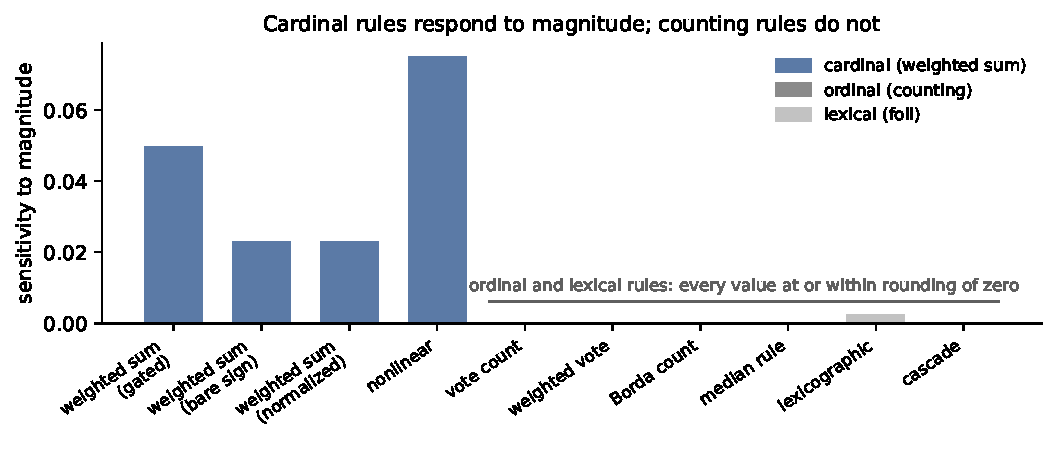
\includegraphics[width=\textwidth]{F5_cardinal_ordinal}
\caption{Only cardinal aggregation reads how strongly a principle
applies. Under a magnitude-only perturbation, which holds every sign and
every within-case rank fixed and changes only the strengths, the four
cardinal rules change their verdicts on $2.3\%$ to $7.5\%$ of cases;
Berman's weighted sum sits at $4.96\%$ with its determinacy gate at
$\tau = 0.2$ and at $2.3\%$ on the bare sign of net force, which is the
clean cardinal reference, the gap between the two being the cases the
gate moves across the determinacy threshold rather than across the verdict.
Every ordinal counting rule changes its verdict on exactly none of them
($0.000$, by construction, having never read a magnitude), and the
lexical foils on effectively none (lexicographic $0.24\%$, cascade
$0.000$). The measurement separates the cardinal family from the other
six rules by roughly a factor of ten at its narrowest. It does not
separate the ordinal rival from the lexical foil, which sit together at
or within rounding of zero; that division is a conceptual one about what
each rule does with the principles it declines to weigh, not one this
instrument reports. Only the cardinal family is faithful to Berman's
picture of principles that weigh rather than rank.}
\label{fig:f5-cardinal}
\end{figure}

Half of that result is definitional, and Part IV said as much of the
lexical comparison. The point extends to the ordinal class. That a rule
which reads only signs and ranks scores zero under a probe that moves
only magnitudes is not a rounding and not a finding. It is what such a
rule does, by construction, when a magnitude changes. The non-definitional
half is that every rule in the cardinal family responds
substantially, at rates from two to seven percent where the ceiling on
the entire far side is a quarter of one percent, and the requirement credits
exactly that.

The second caveat concerns what the probe does not show. By a factor of about ten at its narrowest, the cut it makes is between the
cardinal rules and everything else. It does not separate the ordinal rules from the
lexical ones, and it is not asked to. On this measurement the two are
alike, both at or within rounding of zero, and lexicographic ordering is
if anything marginally the higher of the two. Into a rival and a foil, the division of that far side is a conceptual one,
resting on what each rule does with the principles it declines to weigh and
on how each stands toward the theory, not a division this instrument
reports. The figure shows exactly that: four bars with height and six lying on the
axis. No more should be read off it.

\subsection{Inside the Weighing Family, the Form Is Idle}

The property that makes the family the family, sensitivity to how
strongly a principle applies, is met by every cardinal rule tested and by
no ordinal or lexical rule. That is a narrower claim than it may look, and the narrowness is
deliberate. Only one of Part III's four requirements is measured rule by
rule here. Well-definedness is a property of the weight vector rather than
of the aggregation rule, and by construction it is constant across all ten. For the weighted sum alone, noise tolerance and the margin over the
hierarchical Hart are measured, and for a reason given below they could not
be measured like-for-like across the whole set in any event. But the requirement that carries Berman's
distinctive commitment is exactly the one the probe measures, and it
comes out as a property of the class rather than an artifact of Simple
Additive Weighting's functional form.

In this battery the weighted sum's own reference figure is a determinacy
margin of $+0.268$ over the hierarchical Hart, the charitable comparator of Part IV. It sits with the margins already on the record: $+0.272$
for the stipulated engine in Part IV, and the mechanism cluster of Part
VI, uptake near $0.27$, reliance $0.291$, strategic $0.283$, appointment
$0.284$. Nothing in this Part's battery moves it.

Of the two comparisons the battery supplies, one has to be set aside, and
setting it aside is the methodological point on which the rest of this
Section depends. A \textit{gated} rule holds a threshold below which it
declines to decide and reports the case as unresolved. An \textit{ungated}
rule has no such threshold. As run here the weighted sum is gated: at $\tau = 0.2$ it decides $86.3\%$
of cases and reports the remaining $13.7\%$ as unresolved. Every other rule
in the set is ungated, so it converts every case into a verdict, breaking
ties by whatever its construction supplies, and posts a determinacy rate of
$1.000$ (Borda alone falls short, at $0.996$, and its shortfall is exact
rank ties). That is not more law. It is the same law with the cases in
equipoise relabeled as decided.

That inflation is easy to quantify. Of these same cases the hierarchical
Hart decides $59.4\%$. Against it the ungated rules show an apparent
determinacy margin of $+0.406$ where the weighted sum's margin is
$+0.268$, and the extra fourteen points are bought entirely by never
abstaining.

What makes this a methodological correction rather than a defense of
Berman's rule is where the inflation lands. On the faithful members of the
cardinal family it falls exactly as it falls on the foils.
The sign variant and the normalized variant of the weighted sum both post
$1.000$ for precisely the reason lexicographic ordering and cascade do,
and the sign variant is the bare-sign rule that Part III takes as the
faithful baseline and that Berman himself endorses. On continuously distributed activations exact equipoise has probability
zero, so Berman's own preferred rule never abstains and posts a perfect
determinacy rate for no substantive reason at all. Across a gated and an
ungated rule, therefore, no determinacy figure and no margin over the
hierarchical Hart is like-for-like, and none is offered here as though it
were.\footnote{That the bare sign of net force is Berman's own faithful
baseline is \textit{supra} Part~III.A; see Berman, \textit{Practices},
\textit{supra} note 7, at 331 (an aggregative system ``could incorporate
thresholds or eschew them'').}

The second comparison the battery supplies is verdict agreement, the share
of cases on which each rule returns the weighted sum's own verdict, and it
carries a ceiling that has to be stated before the figures can be read at
all. At $0.863$, the bare-sign variant's raw agreement is numerically
identical to the weighted sum's own determinacy rate, and the identity is
not a coincidence. The weighted sum abstains
on $13.7\%$ of cases and no ungated rule ever abstains, so no ungated
rule can exceed $0.863$ on the raw measure.

Restricted to the cases the
weighted sum actually decides, the sign variant and the normalized
variant return its verdict on all of them. Read raw, the figures invite
the inference that the sign variant \textit{only} agrees with the
weighted sum six times in seven, when in fact it never once departs from
it where the weighted sum speaks.

Read on the cases the weighted sum decides, the figures also contain a
result that does not favor this Part's thesis, and it belongs in the text
rather than in a footnote. Agreement does not track class membership. By
far the most distant are the lexical foils, returning the weighted sum's
verdict on $0.668$ and $0.650$ of the cases it decides, and the theory would
predict exactly that of the thing it defines itself against. But the nonlinear
rule, a faithful cardinal member of the family, agrees on $0.881$, below
every ordinal rule in the set (vote-count and the weighted vote
at $0.886$, Borda at $0.921$).

Properly normalized, the nonlinear rule is the most distant from the
weighted sum of the six distinct in-theory rules, setting the two controls
aside. This Part's claim is therefore about the requirement and about the
class separation the magnitude probe reports. It is not a claim that the
cardinal family is uniformly closer to the weighted sum on verdicts,
because it is not, and this Part does not treat verdict agreement as a
measure of fidelity to the theory.\footnote{Share of cases on which each
rule returns the weighted sum's verdict: SAW-sign $0.863$, SAW-$L_1$
$0.863$, nonlinear $0.761$, vote-count $0.765$, weighted vote $0.765$,
Borda $0.795$, median-sign $0.765$, lexicographic $0.577$, cascade
$0.561$. These raw shares carry a ceiling: the weighted sum abstains on
$13.7\%$ of cases and no ungated rule ever abstains, so no ungated rule
can exceed $0.863$, and SAW-sign reaches it exactly. Restricted to the
cases the weighted sum decides, the shares are SAW-sign and SAW-$L_1$
$1.000$, Borda $0.921$, weighted vote $0.886$, vote-count and median-sign
$0.886$, nonlinear $0.881$, lexicographic $0.668$, cascade $0.650$.}

Two of the ten labels are controls rather than independent evidence, and
saying so keeps the count honest. By construction the normalized variant is
sign-identical to the sign variant, since a positive rescaling of the
weights cannot change the sign of a sum; it is included only to forestall the objection that the result
depends on the scale of the weights. And the median rule coincides with
the bare vote-count on a panel of odd size. Ten labels are eight distinct
verdict rules.

What this Section establishes, then, is that the results of Parts IV
through VI do not rest on Simple Additive Weighting rather than on some
cousin of it. On the linear form Berman's picture does not appear to stand
or fall:
the property the theory is defined by belongs to every rule in the
family, and the normalization and gating variants of his own rule return
his verdict on every case he decides. The scope limit stated at the
outset holds here too. This is established for the defining property and
for these cases. It is not established by running the four mechanisms of Part VI through ten
aggregation rules, which this Part did not do, and a design that did might
well report otherwise.

\subsection{The Disagreements Sit in the Close Cases}

Because both sides of it can be made ungated, the comparison across the
cardinal-ordinal line is the cleanest measurement in this Part. On the
cardinal side here is the bare-sign rule rather than the gated weighted
sum, chosen so that both rules decide every case and the gate cannot
contaminate the contrast. The ordinal side is the counting family.

With every principle carrying exactly equal weight and activations drawn
independently, the two disagree on $15.3\%$ of cases. The equality has to
be exact rather than near, because that is the condition Theorem 5 is
stated under. Part IV measures the same quantity at $15.4\%$ on a separate implementation.
Two independent batteries landing within a tenth of a point is a check on
both, and it is the only check available, since Theorem 5 establishes that the
disagreement is nonzero without fixing how large it is. It is worth being
clear about what the number is not. It is not a claim that either rule is right, and nothing in the design
would support one. It is the share of cases on which the choice between reading magnitudes and
counting votes appears to change the verdict. Berman, shown an early
version of this comparison, called the cardinal-ordinal finding striking,
and added that he had nothing to say about it yet.\footnote{E-mail from
Mitchell N.\ Berman to author (Mar.\ 2026) (on file with author)
(describing ``the finding regarding cardinal aggregation vs ordinal
ranking'' as ``striking'' and as ``interesting and surprising''). The
reaction is to the contrast between weighing and counting, not to the
particular rate reported here.}

With the structure of the cases the rate moves, and one of the two trends
looks robust. As the activations become correlated, the disagreement falls,
and it falls in all nine combinations of ordinal rule and weight
distribution without exception. From $15.3\%$ under independent
activations, the counting rules fall to between $11.5\%$ and $12.2\%$
under the category correlation of realistic cases, in which principles of
the same category tend to fire together, and to $2.9\%$ under full
correlation, where every ordinal rule ends between $1.4\%$ and $3.2\%$.
(Borda runs lower under category correlation, at $5.6\%$ under graded weights
and $7.3\%$ under moderate ones, so the eleven-to-twelve figure is the
counting rules alone. Its equal-weights cell is set aside for the reason given
below.) The fall itself holds for every rule and every weight regime,
including the cells that are set aside, since what contaminates those is
constant across the activation axis along which the fall is measured. The reading is straightforward enough. When a category of principles fires
as a bloc, the side carrying the greater force is generally also the side
with the greater number, and counting and weighing point the same way.

The second trend is weaker and should be reported as such. As the weights
spread out, the counting rules disagree with the bare-sign rule slightly more
often: the bare vote-count runs from $15.3\%$ under equal weights to $15.8\%$
under moderate weights and $17.8\%$ under graded ones, and the weighted vote
from $15.3\%$ to $15.8\%$ to $16.4\%$. Those are movements of two and a half
points and one, across the whole span of weight dispersion the Article tests.

The Borda rule is not reported here, because its equal-weights cell does not
measure what the label says. The implementation converts the weights to their
ranks before scoring, and a vector of identical weights has no ranks to
convert, so the procedure supplies an arbitrary ordering of the nine
principles in whatever sequence they are stored. Under graded weights the
conversion is meaningful and the cell is sound; under exactly equal weights it
is not, and no trend that uses that cell as an endpoint can be
read.\footnote{The defect is confined to this comparison. Borda's
magnitude-probe score is exactly zero in every configuration, which is what
the class separation uses it for, and the ranking it is handed does not affect
a probe that holds ranks fixed.} So the direction in which weight dispersion
moves the cardinal-ordinal gap is reported for the counting rules alone, and
no general law about ordinal aggregation should be read off it.

One convention from Part IV has to be suspended here rather than carried
forward. As the conservative baseline, Part IV banked independent
activations and asked that every figure be read as a floor, because
correlation improves the model's performance. That convention is about the
model's performance, and this quantity is not a performance measure.
For the cardinal-ordinal disagreement rate the convention runs the other
way. Independent activations produce the largest gap, presumably because
principles firing independently produce the close cases where
counting and weighing part company. Along the correlation axis the $15.3\%$ is an upper bound
on this quantity rather than a floor, and the figure for realistic cases
is the middle band.
Carried forward, Part IV's convention would likely lead a reader to misread
the headline in this Article's favor.\footnote{The fall with correlation is monotone
across every rule and weight regime tested, so Part~IV's floor convention
does not carry over to this measurement.}

One further feature of the grid licenses a claim that would otherwise be
rhetorical. In all nine cells, for the bare vote-count and the weighted
vote, the disagreement rate and the opposite-verdict rate are identical to
the last digit. Both rules are ungated, and so is the cardinal
rule on the other side, so every disagreement is a case in which each
rule reaches a verdict and the two verdicts point opposite ways. These are flat contradictions, not cases in which one rule decides and the
other falls silent. Among the four, Borda is the small exception,
abstaining on exact rank ties in about four cases in a thousand.

Where those contradictions sit in the run of cases is perhaps the sharpest
result in this Part. At issue is the size of the net force introduced in Part
II, the balance the weighted sum computes, positive for one side and negative
for the other, so that its size measures how far the case is
from a tie: a large net force is a lopsided case, and a net force near
zero is a case in near-equipoise.

Sort a battery of twenty thousand cases by that quantity and the
disagreements collapse into the closest ones. On the cases where the two
rules disagree the mean size of the net force is $0.35$, against $1.03$
where they agree. On the closer half of the caseload the disagreement rate
is $29.9\%$, against $2.9\%$ on the farther half, and $91.1\%$ of all the
disagreements fall in the closer half. The most
direct statement of the result needs no grouping at all: across those
twenty thousand cases, the largest net force on which the two rules
disagreed anywhere was $1.61$, against an observed maximum of $4.44$.
Nineteen percent of the cases carry a net force above $1.5$, and exactly
four of them are disagreements.

Cut the same sorted caseload into ten equal groups, deciles, the first
holding the closest tenth of cases and the last the most lopsided tenth,
and the profile is the one in Table~\ref{tab:closeness}. Steep as the gradient is, it is a gradient and not a wall: the rate is
still $15.2\%$ at the median case, and only the most lopsided tenth is
exactly zero.

\begin{table}[t]
\centering
\small
\caption{Disagreement concentrates in the closest cases. Equal-count
deciles of the caseload, sorted by the size of the net force.}
\label{tab:closeness}
\begin{tabular}{lc}
\toprule
\textbf{Decile of cases, by net-force size} & \textbf{Disagreement rate} \\
\midrule
1 (closest cases)  & $44.9\%$ \\
2                  & $39.0\%$ \\
3                  & $30.2\%$ \\
4                  & $20.4\%$ \\
5                  & $15.2\%$ \\
6                  & $8.0\%$ \\
7                  & $4.8\%$ \\
8                  & $1.6\%$ \\
9                  & $0.3\%$ \\
10 (most lopsided) & $0.0\%$ \\
\bottomrule
\end{tabular}
\end{table}

That interpretation is the payoff of the Part. When the principles on one
side plainly outweigh those on the other, counting and weighing return the
same verdict, because the side carrying the greater force is generally also
the side with more principles behind it. On those cases magnitude
information is idle and the two rules are interchangeable. It becomes
decisive exactly where the case is close, and that is where a theory of legal content
is under the most pressure to supply an answer at all.

Behind that pattern lies a strongly activated minority of principles
outweighing a weakly activated majority. The sum finds for the minority,
the count finds for the majority, and because both rules decide, the two
contradict one another rather than one of them falling silent. Of that
description the minority half is analytic rather than merely observed. The panel holds
nine principles and exactly zero activations have probability zero, so a
vote-count always finds for a side holding at least five; whenever the
weighted sum disagrees with it, the sum is finding for a side holding
four or fewer. The magnitude half is measured. Where the two rules disagree, the losing
side carries $0.437$ of the total weighted force, against $0.324$ where
they agree. The disagreements would seem to be the cases in which the side
that loses is nearly as strongly supported as the side that wins.

Two limits attach to the result. The zeros are finite-sample zeros and not
entailments. Easy enough to construct is a lopsided case on which the two
rules disagree: five principles activated at $-0.1$ against four activated
at $+1.0$ yields a vote-count that finds negative against a large positive
net force. The observation is that across twenty thousand cases drawn from
nine independent activations none arose above a net force of $1.61$, not
that none can. And rather than the thirty-seed averaging used elsewhere in this Article,
this experiment is a single battery, one seed and one weight vector over
twenty thousand cases. Its overall disagreement rate
of $16.4\%$ is consistent with the thirty-seed grid's $15.8\%$ for the
matched configuration, which is the check available, but the figures
should be read as one battery's.\footnote{The cardinal side of this
comparison is the ungated bare-sign rule, so that both sides decide every
case and the gate cannot contaminate the contrast; cases are sorted by
the size of the net force the weighted sum computes. The figures come from
a single battery of twenty thousand cases at one weight vector rather than
from the thirty-seed averaging used elsewhere in this Article; its overall
disagreement rate of $16.4\%$ is consistent with the thirty-seed grid's
$15.8\%$ for the matched configuration.}

That concentration is arguably what vindicates the magnitude-weighing
requirement, and it supplies the half of the case that Parts III and IV
both flagged as missing. Their caveat was that half of the requirement's
evidence is definitional, since a rank-only rule is blind to a
magnitude-only probe by construction. The concentration supplies the
non-definitional half. The cases on which the blindness matters are the
close ones. On this showing, reading magnitude is not a decorative property
of Berman's rule. It decides
cases, and it decides the hard ones.

What follows is narrower than it may seem, and the narrowness is not a
hedge. Nothing here shows that cardinal aggregation is more
\textit{accurate} in close cases, because the design contains no ground
truth against which either rule could be scored, and this Part is not a
tournament with a winner. Nor does anything here show that ordinal rules are unreliable in any
general sense: on the cases the weighted sum decides they return its
verdict more than four times in five, and on the most lopsided tenth of
this battery they returned it every time. The claim is the narrower one: that the two differ, where they differ, and,
plausibly, why.

\subsection{What This Part Establishes}

Part VI's first question has an answer, and it runs in Berman's favor, though
the answer is narrower than the question. No rule inside the family Berman
endorses is indifferent to the weights, because every member computes each
principle's contribution as its weight multiplied by its activation, so the
weights the mechanisms disagree about enter the verdict directly. The
divergence cannot therefore be made to vanish by choosing a different rule
inside the family.

What is not established is that its rate would be the same under every such
rule. A rule can read the weights and still compress large differences among
them, and this Part did not run the four mechanisms through the ten rules. The
claim is that no member of the family dissolves the divergence, not that every
member reproduces it at Part VI's rate.

Of the whole set, only the unweighted vote-count and the median rule
discard the weights outright. Either would collapse the divergence to
nothing, but only by ignoring the weights altogether, which would abandon
the weighting the theory makes central rather than repair anything. That much is argument rather than measurement.
What is measured is that the defining property belongs to every rule inside
the family, at rates from $0.023$ to $0.075$, and to no rule outside it,
where the ceiling is $0.0024$, and that the separation survives every
weight regime and every activation structure short of full correlation, and that the normalization and
gating variants of Berman's own rule return his verdict on every case he
decides. Parts IV through VI are results about weighing, not results
about Simple Additive Weighting.\footnote{The stronger claim, that the
four mechanisms were carried through the aggregation family and the
divergence survived, is not tested here and is not made. What is
established is the narrower and sufficient claim in the text.}

The second thing this Part establishes concerns the commitment itself. The
one measurement that sorts the family is the measurement the theory is
defined by, the cardinal family sits alone on the weighing side of it, and
the line shows up in verdicts. On that evidence Berman's commitment to
weighing rather than ranking is doing work in his theory that it would not
be doing if the family were interchangeable across that line. It is not interchangeable.

Five limits travel with those conclusions, and collecting them in one place
is better than scattering them. This Part did not cross the four mechanisms
of Part VI with the ten aggregation rules. What it varied was the rule,
against three weight regimes and three activation regimes.

The determinacy figures and the margins over the hierarchical Hart are
not comparable across a gated and an ungated rule, so no such comparison
is offered, and the near-perfect determinacy of the ungated rules is an
artifact of never abstaining rather than a property worth having. The
magnitude probe separates the cardinal family from the other six rules
but does not separate the rival from the foil; that division rests on
what each rule does with the principles it declines to weigh, and this
instrument does not report it. The direction in which spreading the weights moves the cardinal-ordinal
disagreement rate depends on whether the ordinal rule counts or ranks, so
neither direction is a law. And the ordering that separates the classes holds
on independent and category-correlated activations but not under full
correlation, where a magnitude probe has almost nothing left to move. Part
III's five-fold bar is a stronger condition than that ordering, and on the
gated rule that the requirement is scored on, it clears the bar wherever the
ordering holds.

The one comparison this Part had to decline points to what comes next.
Because the weighted sum at $\tau = 0.2$ is the only gated rule in the set,
the determinacy comparison was unavailable, and what makes it the only
gated rule is the threshold. Part VI closed with two questions, and
this Part answers the first. What the choice of rule does control is
whether magnitude is read at all, and that controls real verdicts,
concentrated in the close cases. The second question is whether the
divergence, and the determinacy rates that carry it, are instead
artifacts of the determinacy threshold, the line at which net force
becomes a verdict. That is Part VIII's, and it is likely the last of the modeling choices that
could carry the result.


% Authorship: Claude-drafted, author-revised
\section{The Threshold Governs How Much Law}

The second of Part VI's two questions is whether the divergence among the
mechanisms is an artifact of the determinacy threshold. Stated that way it
invites a second defense, and a defense is arguably the wrong shape for this
parameter. The threshold is the parameter Berman expressly declines to fix. It is not the only quantity this
Article chooses rather than reads off his text. The correlation structure of
the activations is equally a modeling choice, and Section VIII.B finds it
carries more of the substantive results than the threshold does. Unlike
the correlation structure, the threshold is a choice Berman addresses and
leaves open. He writes
that an aggregative system ``could incorporate thresholds or eschew
them,'' commits to neither, and has pressed the point
directly.\footnote{Berman, \textit{Practices}, \textit{supra} note 7, at
331 (an aggregative system ``could incorporate thresholds or eschew
them''). In correspondence he confirmed that his claim is that some
threshold is available to such a system, not that one is required.
E-mail from Mitchell N.\ Berman to author (Mar.\ 2026) (on file with
author). Nothing here rests on the correspondence; the published text is
sufficient and the correspondence confirms it. That the faithful baseline
is accordingly the bare sign of net force, $\tau = 0$, is \textit{supra}
Part~III.A; see also \textit{supra} Part~IV.A.}

The quantity itself is easy to state. Net force is the signed number the
weighted sum returns, positive for one side of the case and negative for
the other, and a case counts as determinate when the size of that number
exceeds $\tau$. Below $\tau$ the model reports the case as unresolved
rather than deciding it by a hair. At $\tau = 0$ nothing is withheld and the bare sign decides everything. At
$\tau = 0.2$, the value used throughout this Article, about one case in
seven comes back unresolved. As a modeling decision, Parts III and IV both
flagged that value and deferred it here.

So the threshold is the Article's rather than Berman's, and a parameter
the theory declines to fix calls for a statement of scope rather than a
defense: the results reported so far that it governs, set against the
results it does not. The answer would seem to divide cleanly. On the evidence below, the threshold governs how much of the law comes out
determinate, and it governs that almost completely. It does not appear to
govern the model's substantive properties, which turn on the
structure of the cases rather than on where the line is drawn. Everything
in this Part, the answer to Part VI's second question included, would seem
to follow from that division.

This Part takes Berman's concession at full strength and reports that
the model cannot repair it, since nothing internal to the model selects a
positive threshold. It then measures what the threshold does control,
returns to the one comparison Part VII had to decline, and states how much
is left standing for the second finding.

\subsection{A Choice the Theory Does Not Make}

On this Berman's published text leaves the threshold open, and asked about
it he confirmed that his claim is that some threshold is available to an
aggregative system, not that one is required. In Part III the consequence
is recorded: the faithful baseline is the bare sign of net force, and a
positive $\tau$ is a confidence gate this Article imposes for reasons of
its own. Nothing about the concession is grudging. It is correct, and the rest of
this Section is what the model says once it is taken seriously. Whether
some future version of the theory would want a threshold is a question the
model cannot reach.

For every mechanism tested, sweep $\tau$ upward from zero and the share of
cases decided falls smoothly and monotonically. It begins at
$D(0) = 1.000$, the value deciding by the bare sign amounts to:
exact equipoise has probability zero on continuously distributed
activations, so at $\tau = 0$ every case has a verdict. From there the
curve descends without a kink, a plateau, or an interior optimum,
reaching between $0.794$ and $0.828$ at $\tau = 0.30$ depending on the
mechanism. This is not a feature of the draws. On independent activations the determinacy
rate has a closed form in $\tau$, proved as Theorem 4 in Part IV and verified
again here on a finer grid running down to $\tau = 0$, which the simulation
matches to a maximum error of $0.0106$. The form is a Gaussian tail in
the ratio of the threshold to the dispersion of net force, and that
dispersion is $\sigma_F = 1.141$ on the weight vector used
throughout.\footnote{The closed form is
$D(\tau) = 2\left(1 - \Phi(\tau/\sigma_F)\right)$, where $\Phi$ is the
standard normal distribution function and $\sigma_F^2 = \frac{1}{3}\sum_i
w_i^2$ is the variance of net force; here $\sigma_F = 1.141$. This is Theorem~4, \textit{supra} Part~IV.D. Part~IV reports a maximum
error of $0.006$ over the coarser grid used there, which starts at $\tau =
0.05$; verified again on the finer grid of this Part, which runs down to
$\tau = 0$, the residual is $0.0106$ over $\tau \in [0, 0.40]$. The theorem is not degrading, the grid is denser and reaches further toward
the origin. Both residuals measure the quality of the normal approximation the
closed form rests on rather than the fidelity of the implementation. The form
is derived for independently drawn activations and does not carry over to
correlated ones, which is why the threshold sweeps of this Part are conducted
on independent draws. The global sensitivity analysis of Section VIII.B is
not; it varies the activation correlation deliberately and so tests something
else. The formula is separable in the threshold and the weights, which meet
only through the ratio $\tau/\sigma_F$, and Section~VIII.B is consistent with
that separability
independently: the threshold's interactions with the other three inputs carry $0.028$ of the
variance. That decomposition runs over a design sweeping the activation
correlation from zero to $0.9$, so it spans the region where the margin over
the hierarchical Hart reverses sign, which Part IV reports at $-0.054$ under
category correlation. What it shows is that the threshold does not govern
whether that requirement holds. The activation structure does.}


A parameter with a privileged value would have something on its response
curve to point at: an elbow where the returns change, a saturation point, a
discontinuity where the model's behavior changes character. This curve
has none of that. Between $\tau = 0$ and $\tau = 0.30$ it loses about
seven points of determinacy for every $0.10$ of threshold and does
nothing else. On the curve's own evidence any value in that range would seem as
defensible as any other, and the default of $0.20$, at which the stipulated
engine decides $86.2\%$ of cases, is a convention rather than a discovery. Figure~\ref{fig:f3-threshold} shows the curve for the
stipulated engine and for the three mechanisms the sweep rebuilds.

\begin{figure}[t]
\centering
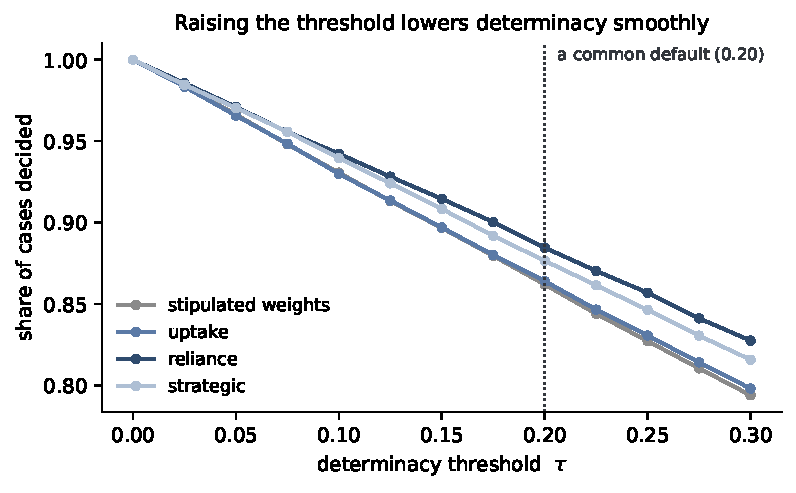
\includegraphics[width=\textwidth]{F3_threshold_choice}
\caption{The determinacy threshold is a choice the theory does not make.
A case counts as determinate when the size of its net force exceeds the
threshold $\tau$. Raising $\tau$ lowers the share of cases decided
smoothly and monotonically for every mechanism, from $1.000$ at
$\tau = 0$ to between $0.794$ and $0.828$ at $\tau = 0.30$, with no kink,
no plateau, and no privileged value anywhere on the curve; $0.20$ is a
common default and is marked for reference. The curve has a closed form
in $\tau$, which the simulation matches to a maximum error of $0.0106$.
Berman's text permits an aggregative system to eschew thresholds
altogether, so the faithful baseline is the bare sign of net force, the
$\tau = 0$ end of this figure, where determinacy is at its maximum.
Curves are thirty-seed means for the stipulated engine of Part~IV and for
the uptake, reliance, and strategic mechanisms of Part~VI; the
appointment mechanism's weights come from a separate simulation this
sweep does not rebuild. All four requirements of Part~III hold across the
whole range for each of the three emergent mechanisms plotted.}
\label{fig:f3-threshold}
\end{figure}

A reader may reasonably ask whether some criterion outside the curve
picks a value. Two are available, and they do not agree. A per-case
robustness criterion asks which verdicts survive perturbation of the
weights and sets the band to discard exactly the cases a small error
would flip; across thirty seeds it recommends $\tau^{*} = 0.267$ (standard deviation
$0.010$). A cumulative criterion asks instead at what $\tau$ nine in ten of
the still-determinate verdicts are robust. It recommends $0.075$ (standard
deviation $0.008$), and that figure is probably biased low, since it averages the fragile cases near the margin in with
the safe interior. The two are not two ends of one interval. They answer different questions and land three and a half times apart, so
neither can plausibly be read as fixing the other, and the conventional
$0.20$ sits between them, below the per-case value and above
the cumulative floor.\footnote{The per-case criterion perturbs the
weights with Gaussian noise of standard deviation $0.10$, calls a verdict
robust when its direction survives in at least ninety percent of draws,
and takes the smallest net force at and above which verdicts are reliably
robust: $\tau^{*} = 0.267$ (sd $0.010$) across thirty seeds. The
cumulative criterion asks instead at what $\tau$ ninety percent of all
still-determinate verdicts are robust, and returns $0.075$ (sd $0.008$).
The per-case value scales with the assumed noise, $\tau^{*} \approx 2.67$
standard deviations of it, and moves with both undefended choices: across
assumed noise of $0.05$, $0.10$, and $0.15$ crossed with confidence
levels of ninety-five and ninety percent, it runs from $0.137$ to
$0.495$, with the conventional $0.20$ above the recommendation in two of
those six cells and below it in four (eight-seed means).}

Neither derivation is unconditional, which is the sharper point. Rather than a constant, the per-case value is a multiple of the assumed
weight noise, $2.67$ standard deviations of it. So it moves with both the
noise scale and the confidence level one assumes, running from $0.137$ to
$0.495$ across the plausible grid. The robustness analysis fixes a
confidence level and a noise scale. It does not fix a number.

The last resort would be to let the model choose. It cannot, and for a
structural reason rather than a computational one. Because determinacy is
monotone decreasing in $\tau$, the determinacy-maximizing threshold is
exactly zero, and there is no interior optimum for any procedure aimed at
deciding more cases to find. Every positive threshold is bought by
declining to decide cases the model could decide. That is a defensible
purchase if activation is evidence relative and a court should not treat
a hair's-breadth balance as settling a question, but it is a purchase
made on grounds outside the model.\footnote{$D(\tau)$ is monotone
decreasing for every mechanism tested: for the stipulated engine
$D(0) = 1.000$, $D(0.20) = 0.862$, $D(0.255) = 0.832$. A procedure
selecting the threshold by maximizing how much law the model declares
determinate would therefore return the bare-sign rule, which is Berman's
own baseline and not a positive threshold at all. A procedure that
instead lets the model calibrate the threshold against its own verdicts
returns a value with no variance across seeds, the signature of a
self-referential fixed point rather than of an optimum.}

The theory does not fix the threshold and the model does not fix it
either. It is a choice, and this Article makes it at $0.20$ for
convention rather than for cause. After that, the Article owes not a
justification of the number but an account of its work.

\subsection{How Much, Not Whether}

A parameter the theory leaves blank is a liability in proportion to what
it controls, so the question is what varies when the threshold varies.
Here the instrument is a global sensitivity analysis, which apportions the
variance in an output among four inputs varied together: the threshold,
the dispersion of the weights, the correlation among the principles'
activations, and the share of principles carrying no weight at all, called
sparsity below.
Unlike moving one knob at a time from a fixed starting point, this
measures each input's contribution across the whole space rather than at
one location in it.\footnote{First-order and total-order variance shares
are Sobol indices on a Saltelli design of $8{,}192$ base samples, with
total-order indices by the Jansen estimator and $95\%$ intervals from
$2{,}000$ bootstrap resamples; the implementation reproduces the analytic
indices of the Ishigami benchmark to a maximum error of $0.0002$. The
inputs vary over: threshold $[0.05, 0.30]$, weight dispersion
$[0, 0.30]$, activation correlation $[0, 0.9]$, and share of principles
zeroed, from none to four of nine. The threshold range starts at $0.05$,
so the bare-sign baseline is not inside this variance budget. Each
evaluation runs the same fixed stream of $8{,}000$ cases, so a difference
in output can come only from the four inputs. For a dominant input the
first-order estimate is noisy, its interval running from $0.462$ to
$1.210$, so the tight total-order index of $0.849$ (interval $0.827$ to
$0.871$) rather than the first-order estimate of $0.822$ is the reliable
measure of dominance. The first-order shares sum to about $0.96$, so the
model is nearly additive here.}

On the determinacy rate the threshold dominates, and the point is
conceded without qualification. Across the four inputs varied together, its
total-order share of the variance is $0.849$, with a $95\%$ confidence
interval from $0.827$ to $0.871$. Activation correlation is a distant second at
$0.156$, sparsity third at $0.023$, and weight dispersion effectively
nothing at $0.008$. As far as it goes, the sharpest form of the worry is therefore correct: how
much law this model declares determinate is very nearly a function of where
the line is drawn. Every determinacy figure in this Article should be read
with that in mind.

Run the identical decomposition, with the threshold threaded through in
the same way, on the two substantive outputs, and the ordering reverses.
On the margin over the hierarchical Hart the threshold's first-order
share falls to $0.176$ while activation correlation rises to $0.810$. On
the magnitude probe the reversal is wider still, $0.020$ against $0.919$.
On this evidence the threshold's grip would appear to be specific rather
than general. It reaches how much law comes out determinate. It does not
reach how the decisions look once made.
Figure~\ref{fig:f4-sensitivity} sets the two decompositions side by side.

\begin{figure}[t]
\centering
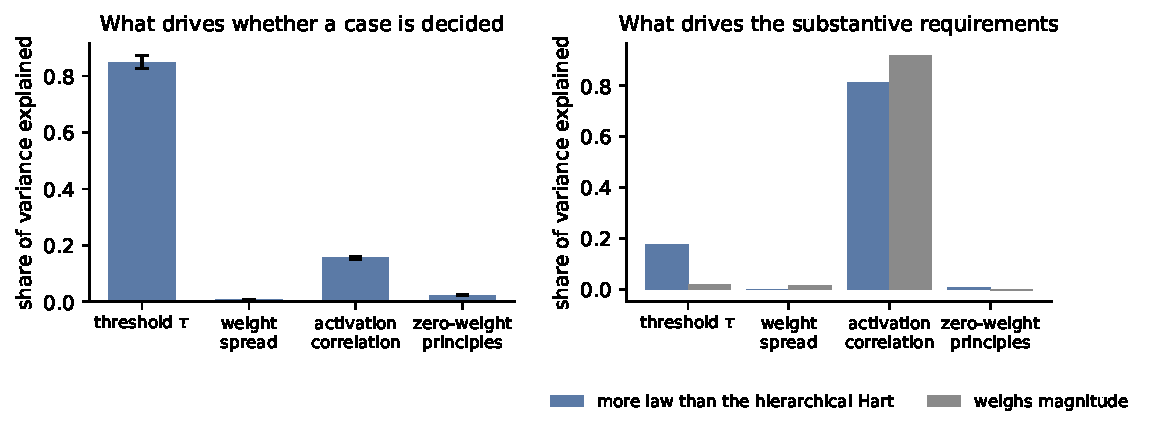
\includegraphics[width=\textwidth]{F4_sensitivity}
\caption{What the threshold governs. A global sensitivity analysis
apportions the variance in each output among four inputs varied together:
the threshold, the weights' dispersion, the correlation among
activations, and the share of principles carrying no weight.
\textit{Left}: for whether a case is decided at all, the
threshold dominates, taking a total-order variance share of $0.849$
($95\%$ confidence interval $0.827$ to $0.871$), against $0.156$ for
activation correlation, $0.023$ for sparsity, and $0.008$ for weight
dispersion. \textit{Right}: for the substantive requirements the ordering
reverses. On the margin over the hierarchical Hart the threshold's
first-order share is $0.176$ against activation correlation's $0.810$,
and on the magnitude probe $0.020$ against $0.919$. The left panel
reports total-order shares, which include each input's interactions with
the others; the right panel reports first-order shares from a smaller run
and should be read as a ranking rather than as precise shares. On that
smaller run the threshold takes $0.635$ of the determinacy variance
against activation correlation's $0.267$, so the reversal holds within a
single design. The threshold governs how much law comes out determinate.
It does not govern whether the model's substantive properties hold.}
\label{fig:f4-sensitivity}
\end{figure}

Before anything is drawn from it, the comparison has to be made
like-for-like, and the reversal is measured inside a single panel rather
than across two runs. In that panel the threshold's first-order share of the
determinacy variance is $0.635$ against correlation's $0.267$, so the
ordering flips between outputs measured the same way on the same design.
Two limits travel with it. The sample is small, so the figures should be read as a ranking rather than
as precise shares. And the magnitude probe varies so
little across this space that its decomposition is only weakly
informative, which leaves the Hart-margin panel to carry the
point.\footnote{The comparison across outputs uses a smaller design of
$256$ base samples and $1{,}500$ cases per evaluation, since only the
ordering is at issue. First-order shares, by input and output: determinacy
rate, threshold $0.635$ and activation correlation $0.267$; margin over
the hierarchical Hart, $0.176$ and $0.810$; magnitude probe, $0.020$ and
$0.919$. The left panel of Figure~\ref{fig:f4-sensitivity} reports
total-order shares from the large design and the right panel first-order
shares from this one, so $0.849$ and $0.176$ are not two measurements of
the same kind; the within-panel figures just given are. Activation
correlation moves the correlation and the scale of the activations
together, and weight dispersion and sparsity both act on weight
magnitudes, so the smaller shares are best read jointly rather than as
cleanly separate effects.}

The reversal has a cause, and naming it turns a report into an
explanation. Deciding a case at its highest-ranked applicable tier, the hierarchical
Hart of Part IV consults no threshold at all, so its determinacy rate
does not move with $\tau$ while the weighted sum's does.
Raising the threshold therefore displaces the margin between them by
exactly the amount it displaces determinacy: over $\tau$ from $0$ to
$0.30$ the determinacy rate falls by $0.206$ and the margin over the
hierarchical Hart falls by $0.206$. The threshold would seem to shift the margin without shaping it. What shapes it is the correlation structure of the
cases, moving the weighted sum and the Hart baseline by different
amounts and so fixing how large the displaced quantity is in the first
place.\footnote{Within a fixed activation regime the margin is the
determinacy rate less a constant, since the hierarchical Hart's rate is
invariant to $\tau$: across $\tau$ from $0$ to $0.30$ both fall by
$0.206$, from $1.000$ to $0.794$ and from $+0.407$ to $+0.201$
respectively. Across the sensitivity sweep the baseline is not constant,
because activation correlation moves the Hart rate as well as the
weighted sum's, which is why correlation takes the larger share of the
margin's variance while the threshold merely displaces it.}

Across this Article's claims, the threshold sets the volume of law and
almost nothing else. The weighted sum's margin over the hierarchical Hart,
and its sensitivity to magnitude rather than rank, turn on how the cases are
structured. A reader who thinks the threshold was chosen badly is
entitled to a different determinacy rate. That reader is not thereby
entitled to a different answer on any of the four requirements, and the last Section of this Part reports what happens when the threshold
is swept across its whole defensible range.

\subsection{The Gated and the Ungated}

Part VII declined one comparison and said why it had to. Except the gated weighted sum, every rule in its battery is ungated, so
each converts every case into a verdict and posts a determinacy rate of
$1.000$.
Against the hierarchical Hart's $59.4\%$ on that battery the ungated
rules show an apparent margin of $+0.406$ where the gated weighted sum
shows $+0.268$. Part VII named the inflation a threshold artifact and
handed the diagnosis here.

The diagnosis is that $+0.406$ is a point on this Part's curve. Nothing
about it is a property of ordinal aggregation or of lexical priority. It
is the margin over the hierarchical Hart at $\tau = 0$. Read
off the threshold sweep run here, on the stipulated engine and a
different battery of cases, the margin runs from $+0.407$ at $\tau = 0$
through $+0.269$ at $\tau = 0.2$ to $+0.201$ at $\tau = 0.30$. The
ungated rules' apparent fourteen-point advantage is the distance between
two points on that curve, and two runs sharing no cases reproduce the
$\tau = 0$ value to within a thousandth.\footnote{\textit{Supra}
Part~VII.B. The hierarchical Hart decides $59.4\%$ of that battery, so
the ungated rules' determinacy of $1.000$ yields an apparent margin of
$1.000 - 0.594 = +0.406$ against the gated weighted sum's $+0.268$ at
$\tau = 0.2$. This Part's sweep, on the stipulated engine over a
different battery and thirty seeds, puts the margin at $+0.407$ at
$\tau = 0$, $+0.269$ at $\tau = 0.2$, and $+0.201$ at $\tau = 0.30$. Two
independent runs reproducing the same figure to a thousandth is what
identifies $+0.406$ as the $\tau = 0$ point on a curve rather than as a
property of any rule.}

Where the artifact lands makes this a correction rather than a defense. On the faithful members of the cardinal family it falls exactly as it falls
on the lexical foils, and it falls hardest on the rule Berman himself endorses.
Because exact equipoise has probability zero, the bare-sign rule of Part
III never abstains, so it posts a perfect determinacy rate and the full
$+0.406$ margin for no substantive reason whatever. Berman's
own baseline is the most inflated rule in the battery.

The general rule this yields is probably what a later reader needs. A determinacy
rate and a margin over the hierarchical Hart are properties of a rule and
a threshold together, never of a rule alone. Any figure of either kind
reported in this Article carries a threshold with it, and comparing two
such figures across rules gated differently compares the gates. The
remedy is not to prefer one setting over another. It is to state the
setting alongside the number, as this Article does, and to
note that the closed form given above converts any such figure to any other threshold
directly.

\subsection{What the Threshold Leaves Standing}

Rebuilding the emergent weights once per seed and sweeping only the
evaluation threshold, from $\tau = 0$ to $\tau = 0.30$ in steps of
$0.025$ over thirty seeds, the four requirements of Part III continue to
hold at every threshold for each of the three emergent mechanisms the
sweep rebuilds, including at Berman's own $\tau = 0$. The requirement
that comes closest to its criterion does so at that baseline, for a
reason Part VII supplies: the magnitude probe scores lower on an ungated
rule than on a gated one, $0.0229$ against $0.0496$, because a gated rule
can also be pushed across the determinacy threshold by a magnitude-only
change, so the five-fold bar is hardest to clear at $\tau = 0$, where the
strategic mechanism clears it on exactly nine seeds in ten. On determinacy the mechanism ordering is invariant as well, reliance above
strategic above uptake, at every threshold above zero; at $\tau = 0$ the ordering is
a degenerate tie, since every mechanism decides essentially every
case.\footnote{The emergent weights are built once per seed, which is the
expensive step, and only the evaluation threshold sweeps, so the
comparison is like-for-like across $\tau$; thirty seeds, $\tau$ from $0$
to $0.30$ in steps of $0.025$, $800$ cases per seed. The requirements are
scored per seed as in Part~III and counted as holding at a threshold when
at least nine seeds in ten pass; the determinacy ordering is invariant for
every $\tau \geq 0.025$. The appointment mechanism's weights come from a
separate simulation this sweep does not rebuild, so it is not carried
through the threshold grid; its noise tolerance is the narrowest of the
four at the default threshold, and this Part makes no claim about its
behavior elsewhere. On the noisier critical-uncertainty measure the
ordering is not strictly invariant, which is reported rather than relied
on. On magnitude-weighing at $\tau = 0$ the per-seed pass rate is
$0.900$ for strategic and $0.967$ for the stipulated engine, against the
stability criterion of $0.9$; see \textit{supra} Part~VII.A on the gated
and ungated magnitude scores.}

One requirement is threshold-sensitive, and the sensitivity attaches to the
stipulated engine rather than to any of the emergent mechanisms. As the threshold rises, the
engine of Part IV, whose weights are hand-set rather than grounded in any
practice, has a critical uncertainty that falls from $0.146$ at $\tau = 0$ to
$0.071$ at $\tau = 0.175$, where it flattens onto Part III's $0.07$ floor. Its
noise-tolerance verdict falls with it, from every seed at thresholds below
$0.10$ to nineteen of thirty at the Article's default and sixteen of thirty at
$\tau = 0.225$.

Two things should be said about that rather than one. Since the quantity
does not fall away but settles on the line, the sensitivity is a bar
crossing rather than a collapse. And the line is where it is because it was calibrated from this
engine at this configuration: Part III sets the floor just below the lowest of
forty-five configuration means, and that lowest mean is this engine at nine
principles, moderate weights, and $\tau = 0.2$. The engine coming to rest on
the floor is therefore close to arithmetic. The sweep adds that the
approach is monotone in the threshold, and that on the stipulated engine noise
tolerance stops clearing Part III's stability bar somewhere below the default
rather than above it. The practice-grounded weights carry more room and stay above the floor
throughout, though how they would behave at a materially higher floor is
not tested here.\footnote{The stipulated engine's
critical uncertainty falls from $0.146$ at $\tau = 0$ to $0.071$ at
$\tau = 0.175$ and then flattens, sitting at $0.071$ at $\tau = 0.20$ and
$0.072$ at $\tau = 0.25$. Because Part~III's floor is $0.07$, the
per-seed pass rate on noise tolerance becomes unstable once the mean
comes to rest on the floor, falling to $0.53$ at $\tau = 0.225$ and
recovering to $0.67$ by $\tau = 0.30$. It affects the hand-set vector
rather than any practice-grounded one: the emergent mechanisms' critical
uncertainties run between $0.086$ and $0.097$ at the default threshold
and fall no lower anywhere on the grid.}

The divergence itself is computed with no threshold at all, which is the
shortest answer available to Part VI's second question. Part VI's
headline, that the mechanisms reach different verdicts on $36.1\%$ of a
battery of fifty thousand cases, is computed on the bare sign of net
force, with no threshold applied, as is every pairwise rate that Part reports.
The gate does not manufacture that divergence. It suppresses it. Applying the
default gate to the same comparison raises the four-way rate from $36.1\%$ to
$44.5\%$, and the rate climbs monotonically with the threshold across the
range tested, so the headline is the most conservative figure the sweep
produces rather than one bought with a gate.\footnote{Part~VI's cross-mechanism divergence is computed on the
sign of net force under each mechanism's mean weight vector, with no threshold
applied, as is every pairwise rate that Part reports. Part VI reports the
gated counterpart alongside it, $44.5\%$ on correlated activations and
$42.5\%$ on independent ones, and the four-way rate rises with the threshold
throughout the range swept, from $0.361$ at $\tau = 0$ through $0.445$ at the
default to $0.478$ at $\tau = 0.3$. The opposite-determinate figure of
$27.2\%$ applies a gate of its own, requiring each of a pair of mechanisms to
clear $\tau = 0.2$ before their disagreement is
counted. Recomputing the divergence with the gate set to zero
confirms the consequence: the opposite-determinate rate rises to
$36.1\%$ on correlated activations and $31.8\%$ on independent ones,
meeting the disagreement rate exactly in both. The runs are reproducible
from the code and data repository accompanying this Article.}

The gated figure moves the other way, which inverts the objection. As the
threshold falls to zero the opposite-determinate rate rises to meet the
disagreement rate, because with no gate every sign disagreement is a pair
of contradictory determinate verdicts. At Berman's own baseline the two
coincide at $36.1\%$, against $27.2\%$ at the default. Raising the gate
does not manufacture the contradiction between the mechanisms. It suppresses it, at a cost of about nine points, and a reader who
preferred a lower gate would see a correspondingly wider contradiction.

Part VI set the relocation as conditional on two answers: if the
divergence holds across the family of aggregation rules and across the
threshold, then it is not a feature of one rule or one threshold but of the
theory. Part VII supplied the first, and in Berman's favor. Inside the family he endorses every rule computes each principle's
contribution as its weight multiplied by its activation, so a disagreement
about weights passes through to the verdict by construction. This Part supplies the
second. The divergence is measured with no threshold applied, the four
requirements survive the whole defensible range of thresholds for the
mechanisms carried through it, and the one parameter the theory leaves
blank governs the volume of law rather than its content. The condition is
discharged, and what is left is what the relocation amounts to for a
theory of legal content. That is Part IX's, and it is arguably the question the whole exercise was
for.


% Authorship: Claude-drafted, author-revised
\section{The Problem of Practice}

Everything to this point has been apparatus: a model, its parameters, its
requirements, and a long series of measurements taken against them. It comes
to this. The relocation reported in Part VI is a claim about the kind of
indeterminacy a practice-based theory of legal content can carry, the
difficulty it names is not Berman's alone, and it leaves a defender a choice
among three substantive positions, none of them yet taken by principled
positivism.

\subsection{Discharging the Condition}

Part VI stated the relocation conditionally and named the two conditions.
If the divergence among the mechanisms holds across the family of
aggregation rules and across the determinacy threshold, then the
relocation is not a feature of one rule or one threshold but of the theory.
On the points that were his to win, both conditions have now been answered,
and the answers ran in Berman's favor.

As Part VII established, no rule inside the family Berman endorses is a
candidate for dissolving the divergence. In that family every rule computes
a principle's contribution as its weight multiplied by its activation, so a
disagreement about weights reaches the verdict by construction. Of the
whole battery, the only rules that could blunt it are the ones that discard
the weights outright, and discarding them abandons the weighing the theory
makes central. As Part VIII established, the divergence was never bought with a gate. The
headline is computed on the bare sign of net force with no threshold applied,
and raising the threshold increases the rate at which the mechanisms disagree
rather than reducing it, so the reported figure is the most conservative the
sweep produces.\footnote{\textit{Supra}
Part~VII.D (every rule inside the cardinal family responds to magnitude,
at rates from $0.023$ to $0.075$, against a ceiling of $0.0024$ outside
it, and every such rule computes each principle's contribution as weight
times activation); \textit{supra} Part~VIII.D (Part~VI's headline divergence is computed on the
sign of net force with no threshold applied, as is every pairwise rate that
Part reports; the four-way rate rises with the threshold, from $36.1\%$ at
$\tau = 0$ through $44.5\%$ at the default to $47.8\%$ at $\tau = 0.3$ on
correlated activations).}

With the condition discharged, the relocation is a claim about the theory
rather than about one rule or one threshold. From here on the argument draws on results already reported rather than
adding to them, with one exception noted where it arises. For a theory of
legal content, those results mean four things. The relocated indeterminacy has a shape of its own, and the
shape is not Hart's. The difficulty it names belongs to any theory that
asks practice for quantities rather than for criteria, so it is not
Berman's alone. A defender is left with three positions and no neutral
ground among them. And the whole of it invites objections, the first of
which comes from inside the theory.

\subsection{More Determinate and Less Settled}

On Hart's account the indeterminacy has a shape, and the shape matters as
much as the fact of it. It is \textit{local}: the law runs out in identifiable hard
cases, at the penumbra of a rule whose core is settled, and elsewhere it
does not run out at all. It is also \textit{visible}. Where the law has
run out, the officials applying it can tell that it has.\footnote{Hart,
\textit{supra} note 1, at 124--36 (open texture and the inevitability of
discretion in hard cases); \textit{id.}\ at 272 (Postscript).} Neither
feature is incidental. Because Hart's gaps can be located, Dworkin could object to them, and there
is no objecting to an indeterminacy nobody can point at.\footnote{Dworkin, \textsc{Law's Empire}, \textit{supra}
note 4, at 37--43.} Inside a Hartian gap, a judge exercising discretion knows she is exercising
it, and so the discretion thesis is a claim about judicial candor as much as
about legal content. For Dworkin's complaint and Hart's defense alike, the gap has to be
locatable.

On both counts the indeterminacy measured here has the opposite shape. It
is \textit{global} in a particular sense, and the sense needs care. The
divergence is not spread evenly across the law. It concentrates on the cases that turn on the moral principles, which is
where the construals are furthest apart, and the objections below return to what follows from that.

It lacks a boundary a deciding judge could draw from inside her own
construal. Under uptake the moral principles are multiplied by zero
before any judgment about them is consulted, so a case that turns on
dignity does not present to her as a case that turns on dignity. In her construal, the marker that would identify the affected set has
already been discarded. A judge is not wholly without a warning, but the warning is unreliable. Under
every construal the size of a case's net force predicts divergence better than
chance, so the closest cases are also the likeliest to come out differently
under a rival reading.\footnote{This is the one measurement first reported here rather than earlier, and it
re-reads Part VI's divergence battery rather than adding a run. Taking the
size of net force as a predictor of four-way divergence, the area under the
curve is $0.636$ under uptake, $0.711$ under reliance, $0.757$ under
appointment, and $0.901$ under strategic, against $0.5$ for a coin. In the
lowest decile of net force the four structures disagree on between $0.53$ and
$0.89$ of cases; in the highest, on between $0.000$ and $0.158$.} But the warning is construal-relative, and sharply asymmetric. Among the cases
each construal ranks in the top decile of its own net force, a reliance judge
runs a reversal risk of $0.006$ and an uptake judge $0.158$, a factor of
twenty-eight. Of the four, the construal that zeroes the moral principles is arguably the
one whose confidence is worth least, and nothing inside it says so.

The first half of that is good news for Berman. At the Article's default
gate of $\tau = 0.2$, each of the three mechanisms carried through the
threshold sweep returns a determinate verdict in a large majority of
cases: uptake on $86.4\%$, strategic on $87.7\%$, reliance on $88.5\%$,
against the stipulated engine's $86.2\%$. On every mechanism the margin over the hierarchical Hart is positive, and the
margins sit near $+0.27$: uptake $0.271$, strategic $0.283$, reliance $0.291$,
and appointment $0.284$. Two conditions travel with that. The margins are
measured on independent activations, and Part IV reports that the comparison
reverses under the correlated activations used for this Part's divergence
figures, the tiered rule there deciding more by consulting less.
And the four figures are closer together than four independent measurements
would be, since the hierarchical Hart never reads the weights, so each margin
is that mechanism's own determinacy rate less one shared constant.\footnote{Thirty seeds at $\tau = 0.2$, $800$ cases
per seed; determinacy rates $0.862$ (stipulated), $0.864$ (uptake),
$0.877$ (strategic), $0.885$ (reliance). Margins over the hierarchical
Hart at the same setting: uptake $0.271$, strategic $0.283$, reliance
$0.291$, appointment $0.284$, with the stipulated engine between $0.268$
and $0.272$ across batteries (\textit{supra} Part~IV.B, Part~VI.A,
Part~VII.B). The appointment mechanism's weights come from a separate
simulation that the threshold sweep does not rebuild, so no determinacy
rate is reported for it here; its margin comes from Part~VI's own
battery. \textit{See supra} Part~VIII.D.} Berman promised more law than
Hart. On every construal of practice tested, he delivers it.

Now the second half. On the battery of fifty thousand synthetic cases
reported in Part VI, the four weight structures return different verdicts
on $36.1\%$ of cases, and on $27.2\%$ they return opposite
\textit{determinate} verdicts once the default gate is
applied.\footnote{The divergence figures come from a different battery
and a different threshold setting than the determinacy rates above, and
the two are not two decompositions of one run. The determinacy rates are
thirty-seed means at $\tau = 0.2$ over $800$ cases per seed; the
divergence rates are computed over a single common battery of fifty
thousand cases under each mechanism's mean weight vector, with the
$36.1\%$ taken on the bare sign of net force ($\tau = 0$) and the
$27.2\%$ requiring each of a pair to clear $\tau = 0.2$. On independent
activations, the Article's conservative baseline, the corresponding rates
are $31.8\%$ and $19.9\%$. \textit{See supra} Part~VI.C, Part~VIII.D.}
Here the pairing matters. Taken alone, each construal of practice decides between eighty-six and
eighty-nine cases in a hundred, and reports every one of them the same way,
as a net force with a sign. The four of them part
company on more than a third. Individually, they are not indecisive. They
are decisive against one another.

For the argument that follows, the missing signal is the point. Reasoning under one construal of practice, a judge gets a number and a
verdict. She does not get a flag. On the
\textit{Obergefell}-style activation profile of Part VI, nothing in uptake's
output records that reliance, reading the same bench and the same holdings by
a different measure with its own warrant in Berman's text, would have decided
the case the other way. Uptake's number, $-1.154$, arrives with no annotation attached. Only by
running a second construal does the contingency become visible, and that is
an operation the theory gives nobody any reason to perform, because the
theory does not say there is a second construal to run. It says the weights are practice-grounded, and
``practice,'' in the singular, sounds like one thing.\footnote{The claim
is about the model's output. Whether a real judge has other signals
available, a sharp dissent, a lopsided circuit split, a visible drift in
the doctrine, is an empirical question about adjudication that this
Article does not reach. What the model shows is that the trace the divergence does leave in the
quantity the theory identifies as legal content, the size of net force, is
construal-relative and worth much less under some construals than others.}

So the finding, at its strongest: a theory can be more determinate and
less settled at once. On every mechanism, by a margin near $+0.27$, Berman genuinely delivers more
law than Hart, and nothing here suggests he delivers it wrongly. Because the design contains no standard against which any of them could be
wrong, no verdict reported in this Article has been shown to be the wrong
verdict. It has been shown, rather, that the determinacy is \textit{indexed}. Under a
construal it is determinacy, and the theory does not fix the construal whose
determinacy it is.

That claim needs one distinction it has not yet been given. It is not the
claim that there is no fact about which dynamic a given legal system runs on.
There may well be such a fact, and a defender who says so is not contradicted
by anything here. The claim is about the theory: given a complete description
of a practice, principled positivism does not by itself say which feature of
that practice fixes the weights, and so does not by itself determine legal
content. That is a claim about the theory's completeness rather than about the
metaphysics of law, and it is the weaker of the two claims available. Since a
simulation of practice cannot discover which dynamic a real system runs on,
the weaker claim is also the one the evidence supports. Hart's gaps announce themselves.
This one does not.

That is what the relocation does to the debate Berman entered. In the
Hart-Dworkin exchange the currency was the \textit{quantity} of law.
Hart conceded that his theory ran out in hard cases, Dworkin said that
running out in hard cases is running out where it counts, and every
subsequent move was an argument about how much law a source-based account
can deliver. Berman answers that charge, and the margin over the hierarchical Hart is
the answer. What the four mechanisms surface is not a quantity of law at
all but a property of the law delivered, and it is arguably a property
neither party had a name for, because neither theory could produce it. 

On one side a Hartian gap is the theory declining to answer, and it declines
out loud. On the other a Dworkinian right answer is the theory answering, in a way
that invites the objection that the answer is the interpreter's. A verdict that is determinate under one reading of a theory's own grounds and
reversed under another reading the theory equally licenses is a third thing,
and from the inside it looks like the second.

Two things keep that from being a larger claim than the evidence supports.
First, about two-thirds of cases are decided the same way by all four
structures, so the claim is not that the choice of construal decides the
law generally; on the run of cases practice speaks with one voice however
it is read, and what is at issue is a large and substantively serious
minority. 

Second, the margin over the hierarchical Hart is real, holds on every
mechanism tested, and is not taken back by anything said here. Part IV's finding
stands as reported there. The guard that closed Part VI holds as
well. Nothing here impugns the synchronic grounding relation: officials'
taking-up of a principle fixes its weight. Under every mechanism that relation
is intelligible, and under every mechanism it works. The open question is the
dynamics of the changing grounds, and it is likely the openness in the
dynamics that propagates into the verdicts.

\subsection{Criteria and Magnitudes}

The difficulty is not Berman's alone. To say why means saying what his theory asks of practice that Hart's does
not.

For its part, Hart's rule of recognition asks officials to converge on
\textit{criteria} of validity: enacted by this legislature, decided by this court, ratified
by this procedure, contained in this text. The convergence it asks for is qualitative. Downstream of a shared
criterion, officials can disagree about nearly everything, including which
way it cuts in the case in front of them, and the rule of recognition is
satisfied so long as they agree on what counts as a source.\footnote{Hart, \textit{supra}
note 1, at 94--99, 100--10. Hart's own account is not wholly free of
quantity: how much convergence among officials is enough to sustain a
rule of recognition is a question he leaves at the level of ``general''
acceptance, and the Introduction to this Article flags it as one of the
places his framework is silent. The contrast drawn here is accordingly
one of degree in how much quantification a theory demands of practice,
not a bright line between a qualitative theory and a quantitative one.}

Berman asks practice for something else. His weights are magnitudes:
quantities of legal force on a scale, one for each principle, and no
aggregation runs without them. A weight is not a verdict on whether a principle belongs to the system. It
is a number that says how much the principle counts when it collides with
another. 

That is a different demand on the same social fact, and it is strictly harder.
The entailment runs one way. In fixing a magnitude a practice thereby fixes the criterion, since a
principle carrying any weight above zero is a principle that counts and
nothing further need be asked. A practice can fix the criterion and leave the
magnitude wide open, since officials can agree without residue that
dignity is among the considerations a court may properly invoke while
disagreeing, or saying nothing at all, about how much it weighs against
plain text. Magnitude is criterion plus a number. That is the sense in
which the second demand is harder, and not any empirical claim that
officials converge less readily on numbers than on categories; the
empirical claim would need evidence this Article does not supply.

On magnitudes, then, is where the four mechanisms disagree. All four run on the same nine principles and the same category map. None of them proposes a
principle the others have not heard of, and none strikes one from the list.
They differ on how much each principle counts. One
qualification. In the limit a quantity of zero is a disagreement about
membership, and under uptake the four moral principles carry weight
exactly zero. But those zeros are post-cut. The underlying uptake shares are small rather than absent, running from
about $0.35$ to about $0.50$ for the moral
principles against $0.79$ to $1.00$ for the textual and structural ones. At the level of the practice the mechanisms actually
read, the disagreement is about how much, and the disagreement about
membership is downstream of a line the model draws.\footnote{\textit{Supra}
Part~VI.C (the uptake zeros are the weights after the cut separating live
principles from dead ones; on the raw shares the moral tier still carries roughly half the weight of the
textual one, and the worked case
still comes out the other way); \textit{supra} Part~V.A (where the cut
falls governs how many principles count as live).}

Stephen Perry's objection to aggregative accounts was a different one. His
was that the messy and contested practice of diverse judges cannot deliver
weights precise enough for aggregation to yield determinate results.\footnote{Perry, \textit{supra} note 9, at 794; Berman,
\textit{Practices}, \textit{supra} note 7, at 328--30 (the ``rough
weights suffice'' reply).} Berman's reply was that rough weights suffice, and Part IV vindicated him:
the weighted sum absorbs weight error on the order of a tenth without
losing its properties. 

To the difficulty here, though, that reply does not reach. It is not that any
single reading of practice delivers weights too imprecise to use. Each of the four delivers weights precise enough to clear noise tolerance, the
one requirement that tests precision. Part VI reports that it is also the only
one of the four requirements that discriminates among weight vectors at all. It is that
the readings deliver \textit{different} weights, and the distance between
them is not imprecision of the kind the model was shown to tolerate.
Against a tolerance for weight error near $0.10$, measured on the same
$[0,1]$ scale as the weights themselves, uptake assigns dignity a weight of
zero where reliance assigns it $0.95$. That is not error around a value.
It is a different value.

With the generalization come its limits. On this reading any
practice-based positivism that moves from criteria to quantities would
inherit this problem, and the more finely a theory quantifies, the more of
it it inherits. Ask practice only whether a source counts, and you need it determinate on a
yes or a no, and the several intelligible ways of reading one practice will
often agree on that. Ask practice how much a
consideration weighs and you need it determinate on a real number, which
the several intelligible readings will not deliver even where they agree
on the yes or the no. That is arguably what the four mechanisms display: agreement on the roster,
disagreement on the column of figures beside it.

Three limits attach.

First, the claim reaches only theories that quantify. It is not a refutation
of positivism, and it is not an argument that positivism ought not to
quantify, since Part IV showed that quantifying buys the extra law: the margin over the hierarchical Hart is the
payoff for weighing a plurality of principles against a rule that decides
at its highest applicable tier, and a theory that declined to quantify
would forfeit it. The margin should not be attributed to magnitude alone. Against a consensus
Hart the weighted sum wins at every bar above a bare majority, by $+0.270$,
$+0.589$ and $+0.786$ as the bar rises, and draws even only at bare-majority
counting, where the rival decides the most cases. So quantifying does buy an
advantage over counting, everywhere but at the counting rule's most permissive
setting; it does not buy the advantage over a tiered rule by
magnitude alone, since the tiered rule differs from the weighted sum in
plurality as well.\footnote{\textit{Supra} Part~IV.B (the
consensus-Hart curve runs $-0.021$ at a fifty-percent bar, then $+0.270$,
$+0.589$ and $+0.786$ as the bar rises); \textit{supra} Part~VII.A (the
hierarchical Hart differs from the weighted sum in magnitude and in
plurality at once, so no comparison against it localises the margin to
either alone). What magnitude buys is measured separately in Part~VII.C,
as a rate of disagreement with counting rules rather than as a
determinacy payoff.}

Second, Hart is not wholly exempt. His account needs an answer to how much
convergence is enough, which is a quantity, so the difference is one of degree
in how much a theory asks practice to fix.

Third, the argument establishes a demand rather than a failure. Showing that a
theory needs more from practice than its predecessor did is not showing that
practice cannot supply it. It shows where the next argument has to be made.

\subsection{What a Defender Owes}

Since the aggregation works, a defender of principled positivism owes not a
repair to it but an addition. In the first place the theory
supplies a synchronic relation: officials take a principle up and embed it in their
reasoning and their holdings, and their doing so confers its weight. It does
not supply a \textit{diachronic} component, an account of what drives those
takings-up over time. Named that way, the missing piece
sits where the evidence puts it and nowhere else. The four mechanisms are four candidate diachronic accounts, and the
divergence among them is the cost of the theory's silence about which is
right.

One reply comes before any account of the dynamics, and it is the strongest
thing a defender can say here. If the grounding relation is synchronic, a
defender may hold that a principle's weight is fixed by current takings-up,
and that the historical dynamic that deposited the present practice is a
question in legal history with no bearing on legal content. That reply
concedes everything Part VI measured and denies that a diachronic account is
owed at all.

It relocates the question rather than dissolving it. The four mechanisms are
not four histories converging on one present practice. They are four readings
of what a taking-up is, and they disagree about the weights of a single bench
and a single body of holdings taken as they stand. Uptake reads how often a
principle is invoked; reliance reads what still rests on it. A defender holding that
current takings-up fix weight has still to name the current facts that count
as takings-up, and that is the question again in its synchronic form.

Granting that an account is owed, three positions are available. Either the
dynamics do not come apart where it matters, or they do; and if they do,
either one of them governs legal content or none does. Those branches give the
three below, taken in the order a defender is likeliest to reach for them.
Each is a substantive commitment and each has a price. I name them and do not
choose.

\textit{Single out one dynamic}, and defend it as the one real legal
systems run on. Being the closest of the four to Berman's own account, reliance is the
natural candidate, and a defender who took this route would be saying that
weight accrues to principles that prevail in contested disputes and embed
themselves in holdings later relied upon, and not otherwise. The cost is
that it converts a conceptual claim into an empirical bet. At least the bet is a payable one, since the dynamics would leave different
signatures: the mean weight vectors stand at rank
correlations of $-0.78$ and $-0.75$ between uptake and each of the
holdings-reading mechanisms and $+0.93$ within that pair, and real
doctrine either exhibits that pattern or does not.\footnote{\textit{Supra}
Part~VI.B (the rank correlations); \textit{supra} Part~III.A (reliance is
the closest of the four to Berman's own account). Part~X sets out what
testing the bet would require.}

\textit{Deny that the dynamics come apart where it matters}, by arguing
that they converge in actual practice in ways they do not in simulation:
real benches, real dockets, and real doctrines of precedent may bring
invocation and embedding into line even though nothing in the models
forces them together. The cost is that the convergence has to be shown rather than assumed, and
Part VI supplies both halves of the relevant evidence. On one side there is a real convergence, reliance and appointment disagreeing
on $1.8\%$ of verdicts, though the two are not independent constructions and
Part VI reports that their agreement tracks the culture they share. On the
other there is a real opposition, uptake against reliance at $35.3\%$ and
uptake against appointment at $33.6\%$. The reply is available, and it is not free. It also carries a discount that
Part VI itself supplies: the shared moral lean behind the convergence is partly a
category-size effect, since the moral tier holds four principles to the
structural tier's three and the textual tier's two, which limits how much
weight a general convergence thesis can rest on that
result.\footnote{\textit{Supra} Part~VI.C (pairwise disagreement rates on
correlated activations: uptake-reliance $35.3\%$, uptake-appointment
$33.6\%$, uptake-strategic $20.6\%$, strategic-reliance $16.3\%$,
strategic-appointment $14.7\%$, reliance-appointment $1.8\%$);
\textit{supra} Part~VI.B (the category-size concession, and the reading
that the convergence tracks a shared object, holdings, rather than a
shared construction).}

\textit{Accept that they come apart}, and with it the indexing: weights
are indexed to a practice, and legal content is correspondingly indexed.
The cost is a form of relativity about legal content that positivists have
generally wanted to avoid, and there is a specific tension with the answer
to Dworkin. Berman's determinacy margin was offered as the reply to the charge that
positivism delivers too little law. A determinate
answer that holds under one construal of practice and reverses under
another is not obviously the determinate answer Dworkin was asking
for.\footnote{Indexing legal content to a practice is already positivism
and no concession at all; what is new is indexing it to a \textit{construal}
of a single practice, which is the distinction Section IX.E takes up
first. The concession, if made, would attach to the dynamics of the
changing grounds and not to the synchronic grounding relation, which
nothing in this Article disturbs. \textit{See supra} Part~VI.D.} It may
nonetheless be the honest position.

I decline to choose among the three, and the refusal is not evasion. Each
is a substantive commitment about how legal systems in fact work, and a commitment of that kind is the theory's to make. A model can price the options. It cannot pick one.
Picking one would require knowing the dynamic that actually drives the
takings-up in a real legal system, and that is not a question a simulation
of practice can answer about the practice it simulates.

\subsection{Objections}

The first objection is the hardest, and it comes from inside the theory. It
says that what has been reported is just positivism being sensitive to social
facts. A Bermanian will put it this way: of course legal content depends on
which practices obtain, and that is positivism. Where officials take up dignity the law differs from where they do not, and
the fact that four different practices yield four different bodies of law is
the theory working, not the theory failing. Reporting it as a difficulty
confuses the social contingency of legal content, always asserted by
positivism, with an indeterminacy in the theory, something else entirely.

The objection has force only if the four mechanisms model four social
worlds. Whether they do is a question about what the divergence is measured
on, and it needs a careful answer, because the four are not built alike.

Two concessions come first. The mechanisms are separate simulations rather
than four read-outs of one simulated history, and their internal machinery
differs more than an earlier draft of this Part allowed. Uptake decides in
nine-judge panels drawn from four methodologies. Reliance has no bench at
all, resolving its disputes against a fixed exogenous pressure structure.
Appointment replaces cohorts of judges who carry no methodology, and
strategic learns a shared weight vector. Nor do the four draw their case
streams alike: uptake's stream is independent across principles, while the
other three are category-correlated.\footnote{\textit{See supra} Part~III.A
for the four constructions. In the implementation, the uptake bench draws
its stream from a uniform distribution over each principle independently,
while reliance, strategic and appointment draw category-correlated
activations.} These four are not one bench observed four ways, and nothing
below assumes they are.

Because the argument does not require the mechanisms to share their
construction, the concession does not reach it. The argument requires the
divergence to be measured on shared cases, and it is. Each mechanism yields
a weight vector. The divergence rates of Part VI are obtained by taking
those four vectors and running each over one common battery of fifty
thousand cases. At the point of measurement the cases are identical and
only the weights differ. The four mechanisms are instruments of different
construction, and the divergence reports their readings of the same object.

That distinction is the one the objection collapses. A Bermanian who says that
different practices yield different law is describing two legal systems whose
officials behave differently, and about that there is no dispute. Part VI
reports something else: four readings of one set of cases, disagreeing about
what the law in those cases is. Contingency of legal content across worlds is
ordinary positivism and embarrasses no one. Underdetermination of legal
content within a world is what a theory of legal content would need to rule
out, and it is what the divergence measures.

Across the four, Berman's account of the ground of weight does not vary.
His schema stands in all of them: officials take principles up and
embed them, and that confers weight. The mechanisms vary in the takings-up
they count and in how those accumulate over time. That is a question about the
dynamics rather than about the grounding relation.
Uptake tallies invocation events over a history. Reliance accrues on
victories and decays. Appointment reads what survives the turning over of
the bench. Strategic settles wherever a divided bench converges. Four ways
of running one relation forward, and they do not end in the same place.

Three things support that reading. The first is the design. In Part II the weights
were held fixed while the activations varied across two Justices, which is
Berman's own experiment: Burger and Powell read the same statute
differently, and the model locates their disagreement in the activations.
In Part VI the mirror image ran, holding one activation profile fixed and
varying only the construal of practice. Same case, opposite experiment.
Run through the four, the \textit{Obergefell}-style profile returns
$-1.154$ under uptake, $+0.708$ under reliance, $-0.140$ under strategic, and $+0.509$ under
appointment. Here the claim is literal rather than figurative. Those four numbers are one activation profile multiplied by four weight
vectors. The case did not change, the principles did not change, and the activations were held fixed by construction. Only the reading of
``taking-up'' moved. Whatever one thinks of the four simulations that produced the weight
vectors, the worked case is a single object read four ways, and the readings
disagree.

The second is what governs the convergence. Reliance and appointment agree
closely, at a rank correlation of $+0.93$ and a verdict disagreement of
$1.8\%$, and they are not independent instruments: on a given seed both take
their exogenous pressure structure from the same source, and the appointment
mechanism was built with the reliance mechanism in view. What matters is not
that they agree but what their agreement tracks. Part VI decouples the
cultures, so that each reads its own rather than a common one, and the
correlation falls from $+0.83$ to $+0.30$, its dispersion across seeds rising
fourfold.\footnote{\textit{Supra} Part~VI.B. The decoupling test is a separate
run, and its baseline is the $+0.83$ mean of eight per-seed correlations
rather than the $+0.93$ computed between the mean weight vectors.} Hold the
culture fixed and the two readings converge; give them different cultures and
they come apart. That is the pattern a world-and-construal reading predicts
and a four-worlds reading does not, since on the latter there is no separate
culture to hold fixed.

The third is that the gap can be named. If Berman's text picked a construal,
the objection would also be sound. It does not. It says principles are
constituted by the taking-up behaviors of the system's subscribers, and
that the weights are practice-grounded, and it points at both invocation
and embedding without resolving in favor of either; Part VI put the open question in that form. On this reading the Bermanian reply presupposes an answer the theory has
not given.\footnote{What the four mechanisms share is narrower than an earlier draft
claimed: the nine-principle set, the category map, the aggregation rule,
and the common battery of cases on which the divergence rates are computed.
They do not share a bench, a panel structure, or the activation
distribution of the streams from which their weights are formed. The shared
battery is what the argument uses. \textit{Supra} Parts~III.A, VI.A. The worked case is
the \textit{Obergefell}-style profile of Part~VI.C, returning $-1.154$
(uptake), $+0.708$ (reliance), $-0.140$ (strategic), $+0.509$
(appointment); perturbing every activation in it with Gaussian noise,
uptake still opposes both reliance and appointment on $100.0\%$ of draws
at $\sigma = 0.05$, $99.1\%$ at $\sigma = 0.1$, and $87.5\%$ at $\sigma =
0.2$, twenty thousand draws at each level. One concession is
owed: the four mechanisms are separate simulations, not four read-outs
of a single simulated history, so the defensible general claim is that
they construe one \textit{kind} of practice under a shared institutional
setup. It is the worked case, where a single fixed activation profile is
run through four weight vectors, that makes ``one world'' literal, and
the reliance-appointment convergence that licenses reading the four as
construals rather than as worlds.}

A second objection accepts all of that and reaches for the obvious remedy. Why
not simply use reliance? A defender might take reliance, the mechanism Part III calls the closest of the four to
Berman's own account, and let it settle the weights. Two things follow, and
the second probably matters more.

The first is arithmetic. Drop uptake from the comparison and the divergence shrinks without going
away: the largest disagreement between
any two of the remaining structures is $16.3\%$, where the largest with
uptake in the set was $35.3\%$. The relocation survives with a smaller
coefficient. For a theory of what determines legal content, one case in six is still
arguably a serious share of a caseload, and Part VI reported the same
figure as the discount on its own headline.

The second is that choosing reliance \textit{is} the first of the three options set out above. It is a substantive commitment about which dynamic real legal systems run
on, and the theory has not made it and would have to defend it. That is no criticism of the choice, which may
well be the right one. It is a description of what the choice costs.
Picking reliance answers the problem of practice. It does not avoid it.

A third objection says the Hartian validation rule is a strawman, and its
force should be conceded first. A Hartian will say that the rule of
recognition identifies \textit{sources} of law, not conflicting substantive
standards, and that a rule so constructed would never certify both sides of
a single case in the first place. Asking only whether each authority is
valid and which way it points, the validation rule of Part IV is not a rule
any careful Hartian would propose, and a result about its behavior is not a
result about Hart.

Three answers, in ascending order of importance. In framing the conflict problem for positivism, Shapiro and Greenberg set
up that foil, and it is used here as they use it, to state a difficulty a
source-based account has to answer rather than to describe a position
anyone holds. It is offered throughout as a contradiction foil and never
as exegesis of Hart, and Part IV says so where it is introduced. And no determinacy figure anywhere is taken against it. Every determinacy comparison runs against the charitable
\textit{hierarchical} Hart, the rule sorting principles into tiers and
deciding a case at its highest applicable tier, with a consensus Hart reported alongside as a
curve across agreement bars. The margin that Part IV claims, and that the argument
above relies on, is the margin over the hierarchical Hart, and it would
stand unchanged if the validation rule were struck from the Article
entirely.

The concession that follows from all three is one of scope rather than of
substance. The contradiction result of Part IV is a result about a rule of a certain
construction, not one about Hart's theory, and this Article does not claim
otherwise. Its claim is narrower and survives the
objection: a source-based account owes some answer to the case in which
two standards both satisfy its criteria and point opposite ways, and the
weighted sum supplies one that a rule of that construction cannot. A
Hartian who says the rule of recognition would never get into that
position is describing a different answer to the same question, not
showing that the question is idle.\footnote{Shapiro, \textsc{Legality}, \textit{supra} note 6, at
270--75; Greenberg, \textit{How Facts Make Law}, \textit{supra} note~42, at
185--89.
Against the hierarchical Hart the stipulated engine's margin is $+0.272$,
positive on every seed; against the consensus Hart the margin runs from a
dead heat at bare-majority counting to $+0.270$ at a sixty percent bar,
$+0.589$ at seventy, and $+0.786$ at eighty. \textit{Supra} Part~IV.B.}

A fourth objection is that the principle set is stipulated, and it is live and
partly unanswered. As implemented, the nine
principles and the sizes of their tiers, two textual, three structural,
four moral, are the author's choice and not a finding. Part VI already concedes that the
shared moral lean under reliance and appointment is partly a category-size
effect: the moral tier is the largest, so under the correlated
activations of realistic cases it accrues broader aggregate force simply
by being larger. The global sensitivity analysis of Part VIII varies four
inputs, the threshold, the dispersion of the weights, the correlation
among activations, and the share of principles carrying no weight, and
the principle set is not among them. And the divergence runs straight
through the moral tier: uptake zeros it, reliance and appointment lift it
highest, strategic parks it in the middle, so the cases most exposed to
the choice of construal are the morally freighted ones.

Those facts interact in a way that ought to be uncomfortable. The moral tier is the largest of the three, and it is also the tier on
which the mechanisms stand furthest apart. So the same design choice that lets that tier accrue broader aggregate
force under correlated activations may also govern how much divergence
there is to measure. Because the sensitivity analysis of Part VIII does not
vary the principle set, it cannot separate the two effects. A replication that
varies the tier sizes directly can bound their joint contribution.

Restricting the principle set directly is the natural test, and it bounds the
effect. Take the four mean weight vectors and drop columns until the tiers are
equal, two principles apiece, and the four-way divergence falls from $0.361$
to $0.303$. Leave the structural tier at three and cut only the moral tier to
two, and it falls to $0.249$. So tier composition accounts for part of the
divergence, between a sixth and a third of the four-way rate, and not for the
rest: on every restricted set the structures still disagree on roughly a
quarter to a third of cases.

Two limits on that test. It restricts rather than replicates. The weight
vectors were themselves formed under the nine-principle map, so dropping
columns bounds what tier size contributes to the verdicts and leaves untouched
what it contributed to the weights. And a balanced set of three principles a
tier does not exist here, since the textual tier holds only two, so the
balanced variants are six and seven principles rather than nine and are not
like-for-like with the full set.\footnote{Tier composition as implemented:
textual (text, original meaning), structural (precedent, structure,
federalism), moral (dignity, equality, liberty, welfare). The restricted sets
are computed on correlated activations and on the bare sign of net force, as
the $0.361$ headline is; no gated counterpart was run. A second balanced
variant returns $0.297$. The sensitivity inputs are listed \textit{supra}
Part~VIII.B, and the principle set is not among them. The category-size
concession is \textit{supra} Part~VI.B, and the concentration of the
divergence in the moral tier \textit{supra} Part~VI.C.}

A fifth objection is that four mechanisms are only a sample, and it is
conceded. Four construals are a sample of the readings a practice-based theory
could take of its own key term rather than the space of them, and nothing
here rules out a fifth that behaves differently from all four. The limit
cuts both ways. A larger sample could add structures to the three already found. Since each of the three is exhibited by a mechanism that has been built and
run, it could not remove them. The sampling limit bounds
the completeness of the claim, not its truth.

The last objection is that the cases are synthetic, which is conceded and was
flagged at the outset. The cases are synthetic and the practice is simulated. A model of this kind can show what a
theory's structure supports and leaves open; the construal of
practice that describes real adjudication is an empirical question, and no number in this Article answers it, nor would any number drawn from
synthetic cases.

\subsection*{What Remains}

The problem of practice is real, and it is narrow. It is not that
principled positivism fails. The aggregation is sound, the weights can emerge from practice rather than
waiting on a theorist, and the margin over the hierarchical Hart, measured on
independent activations, survives every mechanism tested. The problem is that a theory asking practice for magnitudes has to name the
reading of practice that supplies them. Until it does, its determinacy is
determinacy-under-a-construal, and its verdicts carry a contingency that
nothing in them reveals. That is a smaller and more
tractable problem than the one principled positivism inherited from Hart
and Dworkin: not a question about whether social facts can ground legal
content, but a question about which facts about a single practice do the
grounding, with a measurable consequence attached to each answer.


% Authorship: Claude-drafted, author-revised
\section{Conclusion}

Where do the determinants of legal content come from? On Berman's answer
they come from practice, and this Article has taken that answer literally
enough to build it, run it, and measure what it delivers. Two things
followed, and they pull in different directions.

First, the machinery works. Given faithful weights, the
weighted sum returns one verdict where a rule reading each authority
only for validity returns two. On directly opposed cases the rule contradicts itself every time and the sum
never does, and the sum's half of that is an entailment of the aggregation
form rather than a lucky run. It absorbs weight error of about $\pm 0.09$, and better than twice that
under the correlated activations of realistic disputes, where a paired run
rises from $0.069$ to $0.156$. It reads how strongly a principle applies
rather than where the principle ranks. And against a tiered Hartian
hierarchy it leaves less of the law unsettled, by $+0.272$, positive on
every seed.

That last comparison carries a condition that belongs here
rather than only in Part IV, because it is the one most easily mislaid. The
margin is measured on independent activations. Under the correlated
activations this Article treats as realistic it reverses: the tiered
hierarchy decides $95.6\%$ of cases against the weighted sum's $90.1\%$.
The reversal does not show that a tiered rule finds more law. It shows that
such a rule decides faster by consulting less, bringing $1.83$ of nine
principles to bear and setting aside roughly three-quarters of the force in
play. Determinacy counted on its own rewards foreclosure. That is a reason
to ask what a rule hears before asking how much it settles.

Second, none of this fixes what the law is. Between them, four intelligible
readings of officials' taking-up of a principle produce four weight
structures, three of them distinct. Run over a common battery,
those structures return different verdicts on $36.1\%$ of cases on the bare
sign of net force, on $44.5\%$ once the determinacy threshold is applied, and
opposite determinate verdicts on $27.2\%$. Each clears every requirement the theory imposes, three of them on every
seed and appointment on twenty-six of thirty, its noise tolerance
straddling the floor. They differ not in competence but in
object: uptake reads what officials say, reliance and appointment read
what their decisions leave standing.

Put together, the two findings say something a quantity of law cannot
capture. On this evidence principled positivism is more determinate than Hart and
less settled than it looks. Its determinacy is determinacy under a construal,
and the theory does not fix the construal whose determinacy it is. The mark of a verdict its rivals would reverse is present in the output of
any single reading but unreliable, and it is worth least under precisely
the construal that discards the moral principles. Hart's gaps announce themselves to the judge standing in one.
This contingency does not.

Beyond that, several things one might read in are not in it. No verdict
reported here has been shown to be the wrong verdict, since the design
contains no standard that any of them could fail. For Berman, officials' taking-up of a principle makes its weight what it
is. That grounding relation is intelligible under every mechanism, and
under every mechanism it works. The prior question remains open: what
drives those takings-up over time. That is a gap in the
dynamics, not a flaw in the relation.

On the theory's side three positions remain available, and this Article has
priced them rather than choosing among them. First, a defender may single out one dynamic and defend it as the one real
systems run on. That converts a conceptual claim into an empirical bet.
Second, a defender may deny that the dynamics come apart where it matters.
That denial requires showing a convergence rather than assuming one. Or a defender may accept the indexing and its cost,
a relativity about legal content that positivists have generally wanted to
avoid.

Each is a substantive commitment about how legal systems in fact work, and
a commitment of that kind is the theory's to make rather than a
simulation's. A model of this sort can say what each option
costs. It cannot tell anyone which dynamic actually drives the
takings-up in a real legal system, because the practice it reads is the
practice it built.

So the work that follows is empirical, and it has a shape. The first task
is coding, assigning activation values to the principles at work in real
judicial opinions, so that the aggregation can be run against decided cases
rather than synthetic ones. Berman has already coded one case this way,
\textit{TVA v.\ Hill}, showing both that the exercise is possible and
how much judgment it takes. Whether the exercise scales past a handful of
opinions is the question that would have to be settled first.

The second task is discrimination among the dynamics, and it is tractable
because they leave different traces. Against the two mechanisms
that read holdings, uptake stands at rank correlations of $-0.78$ and
$-0.75$, where those two sit at $+0.93$ with each other. Real doctrine either exhibits that pattern
or it does not. A body of case law where a principle's authority tracks
how often it is invoked would look measurably unlike one where
authority tracks the holdings still standing, and the difference should be
visible to anyone willing to count.

A third implication runs the other way, from the model back toward
institutions. The emergent weights of Part V trace to the composition of the
bench rather than to any winnowing of judges as such. Change the mix of
methodologies enough and the line between the principles that carry weight and
those that carry none moves with it: give the methodology that reaches for the
moral principles a majority of the seats rather than a quarter, and three of
them cross the line while three textual and structural principles cross back. On this account, who sits on a court
would shape not only how particular cases come out but which principles
count as legally weighty at all. That is a stronger claim about judicial
selection than the usual one, and a testable one.

The limits travel with all of it, and there are more than two. The cases
are synthetic and the practice is simulated, so which construal describes real
adjudication is a question no number here answers. Four
mechanisms are a sample of the readings a practice-based theory could take
of its own key term rather than the space of them; a larger sample could
add structures to the three found here, though it could not remove them,
since each was built and run.

Three further limits are specific rather than general, and each attaches to
a particular claim. The margin over the hierarchical Hart holds on independent
activations
and reverses on correlated ones, so it is a claim about a case distribution
and not about the rules alone. The separation between weighing and counting
holds across every weight regime and every activation structure short of
full correlation, where a magnitude probe has almost nothing left to move.
And the tier sizes contribute to the divergence: balancing them at two
principles apiece takes the four-way rate from $0.361$ to $0.303$, and
cutting the moral tier to two takes it to $0.249$, so roughly a sixth to a
third of the divergence is attributable to composition, with the remainder
unexplained by it. No run reported here separates that remainder from the
category-size effect operating through correlated activations.

What remains, then, is narrower than the problem principled positivism
inherited. Between them, Hart left the law running out in hard cases and Dworkin left
the right answer resting on moral interpretation, and Berman's aggregation
genuinely improves on both. The question it puts in their place is which
facts about a single practice do the grounding, with a measurable
consequence attached to every answer. That is the problem of practice. As problems go it is a better one than it replaces, and it is now specified
closely enough to be worked on.


% ============================================================================
% APPENDICES (if needed for law review)
% ============================================================================

% \appendix
% \input{sections/appendix_A_replication}
% \input{sections/appendix_B_sensitivity}

\end{document}
